%% This is file `elsarticle-template-3-num.tex',
%%
%% Copyright 2009 Elsevier Ltd
%%
%% This file is part of the 'Elsarticle Bundle'.
%% ---------------------------------------------
%%
%% It may be distributed under the conditions of the LaTeX Project Public
%% License, either version 1.2 of this license or (at your option) any
%% later version.  The latest version of this license is in
%%    http://www.latex-project.org/lppl.txt
%% and version 1.2 or later is part of all distributions of LaTeX
%% version 1999/12/01 or later.
%%
%% The list of all files belonging to the 'Elsarticle Bundle' is
%% given in the file `manifest.txt'.
%%
%% Template article for Elsevier's document class `elsarticle'
%% with numbered style bibliographic references
%%
%% $Id: elsarticle-template-3-num.tex 165 2009-10-08 07:58:10Z rishi $
%% $URL: http://lenova.river-valley.com/svn/elsbst/trunk/elsarticle-template-3-num.tex $
%%
%\documentclass[preprint,12pt]{elsarticle}

%% Use the option review to obtain double line spacing
%% \documentclass[preprint,review,12pt]{elsarticle}

%% Use the options 1p,twocolumn; 3p; 3p,twocolumn; 5p; or 5p,twocolumn
%% for a journal layout:
%% \documentclass[final,1p,times]{elsarticle}
%% \documentclass[final,1p,times,twocolumn]{elsarticle}
%% \documentclass[final,3p,times]{elsarticle}
%%\documentclass[final,3p,times,twocolumn]{elsarticle}
%% \documentclass[final,5p,times]{elsarticle}
\documentclass[final,5p,times,twocolumn]{elsarticle}

%% if you use PostScript figures in your article
%% use the graphics package for simple commands
%% \usepackage{graphics}
%% or use the graphicx package for more complicated commands
%% \usepackage{graphicx}
%% or use the epsfig package if you prefer to use the old commands
%% \usepackage{epsfig}

%% The amssymb package provides various useful mathematical symbols
\usepackage{amssymb}
%% The amsthm package provides extended theorem environments
%% \usepackage{amsthm}

%% The numcompress package shorten the last page in references.
%% `nodots' option removes dots from firstnames in references.
\usepackage[nodots]{numcompress}

%% The lineno packages adds line numbers. Start line numbering with
%% \begin{linenumbers}, end it with \end{linenumbers}. Or switch it on
%% for the whole article with \linenumbers after \end{frontmatter}.
%% \usepackage{lineno}

%% natbib.sty is loaded by default. However, natbib options can be
%% provided with \biboptions{...} command. Following options are
%% valid:

%%   round  -  round parentheses are used (default)
%%   square -  square brackets are used   [option]
%%   curly  -  curly braces are used      {option}
%%   angle  -  angle brackets are used    <option>
%%   semicolon  -  multiple citations separated by semi-colon
%%   colon  - same as semicolon, an earlier confusion
%%   comma  -  separated by comma
%%   numbers-  selects numerical citations
%%   super  -  numerical citations as superscripts
%%   sort   -  sorts multiple citations according to order in ref. list
%%   sort&compress   -  like sort, but also compresses numerical citations
%%   compress - compresses without sorting
%%
%% \biboptions{comma,round}

\biboptions{compress}



\usepackage{IEEEtrantools}
\usepackage{subcaption}
\usepackage{mycommands}
\usepackage{eqs-one-obj}
\usepackage{eqs-two-obj}
\usepackage{eqs-ct-two-obj}
\usepackage{eqs-three-obj}
\usepackage{eqs-ieee-thirty}

\newcommand{\tabname} {Table}
\newcommand{\tabnames}{Tables}
\newcommand{\figname} {Fig.}
\newcommand{\fignames}{Figs.}
\newcommand{\eqname}  {Eq.}
\newcommand{\eqnames} {Eqs.}

\newcommand{\ALGOSIZE}{\small}

\makeatletter
\newcommand{\verbatimfont}[1]{\def\verbatim@font{#1}}%
\makeatother

\setspacesfigures



\journal{CPMECH REPORT 000001}

\begin{document}

\begin{frontmatter}

%% Title, authors and addresses

%% use the tnoteref command within \title for footnotes;
%% use the tnotetext command for the associated footnote;
%% use the fnref command within \author or \address for footnotes;
%% use the fntext command for the associated footnote;
%% use the corref command within \author for corresponding author footnotes;
%% use the cortext command for the associated footnote;
%% use the ead command for the email address,
%% and the form \ead[url] for the home page:
%%
%% \title{Title\tnoteref{label1}}
%% \tnotetext[label1]{}
%% \author{Name\corref{cor1}\fnref{label2}}
%% \ead{email address}
%% \ead[url]{home page}
%% \fntext[label2]{}
%% \cortext[cor1]{}
%% \address{Address\fnref{label3}}
%% \fntext[label3]{}


\title{Parallel evolutionary algorithm in Go language for single and multi objective optimisation
problems with constraints}


%% use optional labels to link authors explicitly to addresses:
\author[uq]{Dorival~M.~Pedroso\corref{cor1}}
\ead{d.pedroso@uq.edu.au}

\cortext[cor1]{Corresponding author}
\address[uq]{School of Civil Engineering, The University of Queensland, St Lucia QLD 4072, Australia}



\begin{abstract}

This paper presents an evolutionary algorithm employing differential evolution for solving nonlinear
optimisation problems with (or without) multiple constraints and objectives. Some new decision
strategies to compare trial solutions in order to produce a robust code with respect to its ability
to generate the same answer every time it is run is presented. In addition, the combination of good
existent techniques is carefully developed. The third contribution is the design of a strategy to
implement parallel computations in a way that diversity is preserved. A final goal is the handling
of a range of problems involving real numbers only or real numbers and integers. The resulting code
is named \goga~and is written in Go (golang) as free/open source code. Numerical examples are
presented illustrating the capabilities and performance of the algorithm. An ideal speedup is
observed during the parallel computations. Two applications are studied: the topology optimisation
of trusses and the environmental economical dispatch problem in power generation.

\end{abstract}



\begin{keyword}
%% keywords here, in the form: keyword \sep keyword

golang \sep
differential evolution \sep
constraints handling \sep
many objectives \sep
truss optimisation \sep
economic dispatch \sep
parallel computation

%% MSC codes here, in the form: \MSC code \sep code
%% or \MSC[2008] code \sep code (2000 is the default)

\end{keyword}



\end{frontmatter}

%%
%% Start line numbering here if you want
%%
% \linenumbers

%% main text



\section{Introduction}
\label{sec:intro}

Evolutionary algorithms (EAs), including genetic algorithms (GAs), are optimisation techniques with
a good dissemination in engineering and many other areas \citep{gold:89, mwicz:96, deb:01a, tan:05,
coello:07}. These techniques avoid the use of derivatives and can tackle quite complex problems,
including discontinuous functions or objectives that may depend on a mixture of data types (binary,
integer, real). Nonetheless, EAs do not necessarily seek for an exact answer and cannot easily tell
whether the solution has converged or not. Therefore, EAs must be well developed and tested under
several circumstances in order to be reliable and able to output accurate results after every run.

One essential characteristic for a good performance of an evolutionary algorithm is the ability to
maintain diversity during the solution process. Simple GAs in particular suffer from early
convergence when, after a number of iterations, most individuals have very similar genetic data and
cannot easily produce better solutions unless mutation happens. Nonetheless, the control of mutation
in this situation is not straightforward. Several research works discuss this topic in detail and
some present strategies to overcome the problem \citep{gold:87, mahfoud:95, chen:14, elsayed:14}.
This contribution considers one solution known as \emph{crowding approach to niching} inspired by
the algorithms in \citep{meng:08, meng:14}. The diversity in this method is maintained by running
tournaments between randomly selected trial solutions and only replacing the previous candidate if
the new solution wins; the competitors in the tournament are firstly matched with respect to a
minimum distance estimate.

Many important problems in Engineering involve multiple constraints; for example structural
optimisation of frames where the cross sectional areas are always positive quantities and loads may
be unidirectional. Another example is the economic/environmental load dispatch problem where the
capacity of power generators is limited and the available power must compensate the losses (along
the transmission lines)---the power balance.

Methods to handle constraints in evolutionary algorithms range from the use of penalty factors to
classification strategies when comparing trial solutions. The penalty method is often the worst one
because the addition of large numbers to the objective function causes numerical problems. This
paper adopts the classification strategy for constraints and presents an algorithm to treat them in
single and multi objective optimisation problems. The concept of Pareto dominance is then applied to
both the objective values and measures of how close to satisfying constraints a trial solution is.
Interesting studies on constraints handling methods are available in \citep{mich:94, mich:95,
mich:96, deb:00, coello:02, deb:03, vieira:04, galan:09, long:14, hellwig:16}.

Also of great importance are multi objective optimisation problems. For instance, the
economic/environmental dispatch problem mentioned above seeks for a compromise between a minimal
cost and minimal emission of pollutants---two opposing objectives. Algorithms have then been
developed along the years to solve multi objective problems as well \citep{tanaka:95, fonseca:95,
fonseca:98a, fonseca:98b, zit:00, tan:01, deb:01b, deb:02, deb:05, kukko:06b, deb:08, tiwari:08,
deb:10, tiwari:11, qiu:16}.

Real-coded genetic algorithms have been a challenge in the early days; but good solutions were
introduced and studied in \citep{deb:95a, deb:95b, mwicz:96, herrera:98}. A simple attempt that
split a float point number into smaller chunks was also successfully proposed and implemented in
\citep{pedroso:11}. Nonetheless, the performance was not necessarily always the best. The
differential evolution (DE) \citep{storn:95, price:05} on the other hand naturally implements
recombinations of real numbers. DE has proven to be an efficient method and at times even better
than classical genetic operators \citep{tiwari:11}. This behaviour has been observed in the
experiments performed by the research reported here leading to a decision to use DE (for real
numbers only). More details on DE can be found in \citep{kukko:05, kukko:06}.

Parallel computing has become a common technique to solve large scale problems. Moreover, modern CPU
design has focused towards adding multiple computing cores to chips because of power and temperature
limitations in silicon. Therefore, new algorithms have to consider parallel or concurrency
techniques in order to make better use of the computer hardware. For evolutionary algorithms,
concurrency is very natural since trial solutions can be assigned into different groups that are run
in parallel. Besides speeding computations up, this approach may widen the search space and improve
the convergence properties. Nonetheless, care must be taken in order to prevent the loss of
diversity when exchanging data between different groups. Thus, a strategy to implement concurrency
is also investigated and proposed in this paper.

Go (golang) is a recent new programming language created by Google engineers in 2007, including
Robert Griesemer, Rob Pike and Ken Thompson \cite{golang:16}. The language was later made public as
open source in 2009. Go has since grown exponentially attracting a large number of co-developers and
users. The main goal leading to the introduction of yet a new language was the combination of
efficiency (like C/C++) with ease of development (like Python). There are other several innovations
and advantages in Go when compared with mainstream languages such as C/C++/C\#/Java/Python/Ruby/Lua.

One particular innovation in Go is the concept of concurrency that can lead to easy-to-write
parallel algorithms. Another convenient characteristic is the simple development cycle that includes
very fast compilation times and efficient modularity by using packages and sub-packages. Go is a
garbage-collected language, compiled in Go language, and finally, has at times prioritised
practicality over strict conciseness that would be defined by long theoretical justifications.
Nonetheless the language definition is very clear and well thought of---note that the creators have
indeed proven experience on computer language design. This last pragmatic approach makes Go as
pleasing to use as possible while ensuring that the code is well organised, modular and efficient.

The algorithms in this paper are implemented in Go; however they are presented in a general format
that can help the implementation in any other language. The resulting code is available in
\url{https://github.com/cpmech/goga} as free/open source and takes advantage of the native
concurrency features of Go. For historical reasons, the code is named \goga~after `Go genetic
algorithm'; however it only employs genetic operators when dealing with integers. The source code
for all tests, examples and graphs are posted in the same web address.

In summary, this paper presents an evolutionary algorithm for solving optimisation problems with
multiple objectives and multiple constraints. The best ideas collected from the aforementioned
literature are taken into consideration and new algorithms and classification strategies are
developed, including: (1) Pareto handling of constraints without penalty weights; (2)
crowding/niching for diversity maintenance to be used in parallel computations; (3) use of both a
neighbour distance and a crowding distance based on the proposed constraints handling algorithm; (4)
random differential evolution operations; (5) two strategies for exchange of solutions during
parallel executions; and (6) handling of hybrid representations using integers and real numbers.



\section{Problem definition}

The optimisation problem (solved by \goga) considering multiple objectives, multiple constraints, 
and mixed types is defined here in a \emph{general format} by means of
\begin{equation}
\begin{aligned}
& \minimise_{\vx,\;\vksi} && \{f_0(\vx,\vksi), f_1(\vx,\vksi), \ldots\}                  && \text{($N_f$ objectives)} \\
& \subjecto               && u_i(\vx,\vksi) = 0                                          && \text{($N_u$ constraints)} \\
&                         && x_i^L   \leq x_i   \leq x_i^U   \quad(x_i \in \mathbb{R})   && \text{($N_x$ box-constr.)} \\
&                         && \xi_i^L \leq \xi_i \leq \xi_i^U \quad(\xi_i \in \mathbb{Z}) && \text{($N_\xi$ box-constr.)}
\end{aligned}
\label{eqn:optGeneral}
\end{equation}
where $f_i(\vx,\vksi)$ are the $N_f$ objective functions, ${\vx=\{x_0,x_1,\ldots,x_{Nx-1}\}}$ are
the design variables (unknowns) of real type, and ${\vksi=\{\xi_0,\xi_1,\ldots,\xi_{N\xi-1}\}}$ are
the design variables of integer type. Therein, $u_i(\vx,\vksi)$ are auxiliary functions called here
as \emph{out-of-range} (OOR) that are introduced to handle additional constraints with respect to
the essential \emph{box constraints} for $\vx$ and $\vksi$. In this paper, when counting constraints,
the box constraints are not included; hence, if only box constraints are present, the problem is
called \emph{unconstrained}. Hereafter, the acronym OVA is also employed to indicate an
objective-value.

The general form in \eqname~(\ref{eqn:optGeneral}) includes the more \emph{specific problem}
expressed by
\begin{equation}
\begin{aligned}
& \minimise_{\vx} && \{f_0(\vx), f_1(\vx), f_2(\vx), \ldots\} && \text{($N_f$ objectives)} \\
& \subjecto       && g_i(\vx) \geq 0                          && \text{($N_g$ constraints)} \\
&                 && h_i(\vx) = 0                             && \text{($N_h$ constraints)} \\
&                 && x_i^L \leq x_i \leq x_i^U                && \text{($N_x$ box-constr.)}
\end{aligned}
\label{eqn:optReal}
\end{equation}
where $g_i(\vx)$ and $h_i(\vx)$ are inequality and equality constraint functions, respectively.
These two types of constraints can be easily converted into the OOR form using the $u_i$ functions
in \eqname~(\ref{eqn:optGeneral}); the number of OOR functions will then be
\begin{equation}
    N_u = N_g + N_h
\end{equation}

The out-of-range functions $u_i$ must return positive values that become smaller as the variables
$\vx$ and $\vksi$ become closer to satisfying the corresponding constraint. If the solution is
feasible, the OOR function is simply zero. The pursuit of zero OORs has priority over minimising
OVAs as discussed in the next section. Note that the strategy involving the out-of-range function is
one step to effectively handle multiple constraints and, in the proposed evolutionary algorithm,
this method will pull infeasible solutions towards the feasibility region.

To exemplify, in a problem involving two constraints $g_0$ and $h_0$, the ramp function defined by
\begin{equation}
    u_0(x) = \left\{\begin{matrix}
        0       & \text{if $g_0(x) \geq 0$} \\
        -g_0(x) & \text{otherwise}
    \end{matrix}\right.
\label{eqn:OORg}
\end{equation}
can be used for the first constraint and the function defined by
\begin{equation}
    u_1(x) = \left\{\begin{matrix}
        0              & \text{if $|h_0(x)| \leq \EpsH$} \\
        |h_0(x)|-\EpsH & \text{otherwise}
    \end{matrix}\right.
\label{eqn:OORh}
\end{equation}
can be used for the second one. Therein, $\EpsH$ is a small number, but not very small (not machine
precision), that is required to effectively convert the equality constraint into an inequality. This
is necessary in order to allow the algorithm to search within a small gap closer to the equality
constraint. An illustration of \eqname~(\ref{eqn:OORg}) is given in \figname~\ref{fig:OORg} and an
illustration of \eqname~(\ref{eqn:OORh}) is given in \figname~\ref{fig:OORh}.

\begin{figure} \centering
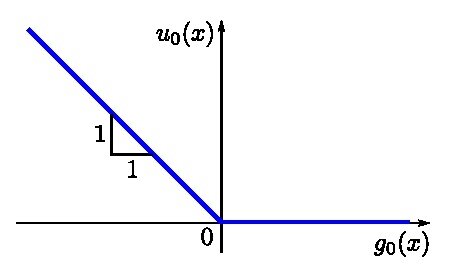
\includegraphics[scale=0.64]{./figs/gfcn.eps}
\caption{Out-of-range (infeasible) function $u_0$ for inequality constraint $g_0$.}
\label{fig:OORg}
\end{figure}

\begin{figure} \centering
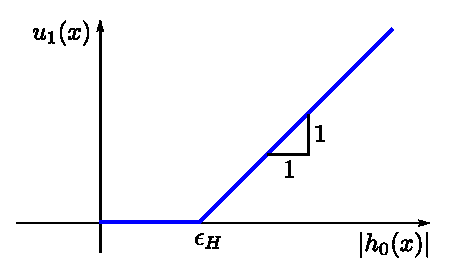
\includegraphics[scale=0.64]{./figs/hfcn.eps}
\caption{Out-of-range (infeasible) function $u_1$ for equality constraint $h_0$.}
\label{fig:OORh}
\end{figure}

The solution of the optimisation problem defined above is obtained in a stochastic manner starting
with the definition of a set of trial solutions indicated by
\begin{equation}
    S = \{(\vx,\vksi)_0, (\vx,\vksi)_1, \ldots\, (\vx,\vksi)_{Nsol-1}\}
\end{equation}
where $(\vx,\vksi)_i$ are the trial solutions and there are $N_{sol}$ of them. For each trial
solution corresponds a vector of objective values $\vf_i$ and a vector of out-of-range values
$\vu_i$. For example, $\vf_A(\vx_A,\vksi_A)$ is the vector of objective values computed with
$(\vx_A,\vksi_A)$.

The minimisation problem considers the concept of Pareto domination \citep{fonseca:98a}. In this
concept, a vector $\vv_A$ dominates another one $\vv_B$ if and only if the following conditions are
satisfied at the same time
\begin{align}
    v_i^A \leq v_i^B && \text{for all}          && i=0,1,\ldots\,N_v-1 \ACR
    v_i^A <    v_i^B && \text{for at least one} && i=0,1,\ldots\,N_v-1
\label{eqn:Pareto}
\end{align}
where $v_i^j$ are the components of the vector $\vv_j$ and $N_v$ is the length of the vector.

Therefore, for multi objective optimisation problems, the word \emph{minimise} in
\eqname~(\ref{eqn:optGeneral}) means to find the Pareto optimal solution satisfying
\eqname~(\ref{eqn:Pareto}) using the vectors $\vf_i$ of objective values. Single objective
optimisation problems are also included in \eqname~(\ref{eqn:optGeneral}); in this case, $N_f=1$.

In this paper, the command \FnParetoComparison~means to apply \eqname~(\ref{eqn:Pareto}) to any two
vectors related to the trial solutions $A$ and $B$ and to find whether solution $A$ dominates
solution $B$ (${A_{dom}=\KwTrue}$), solution $B$ dominates solution $A$ (${B_{dom}=\KwTrue}$), or
none of the above. Thus, it can be implemented in a routine that takes two vector arguments and
returns two Boolean results as follows
\begin{equation}
    A_{dom}, B_{dom} \gets \text{\FnParetoComparison}\;(\vv_A,\vv_B)
\end{equation}



\section{Constraints handling}
\label{sec:constraints}

The method employed to find solutions satisfying all constraints is inspired by the one introduced
in \citep{deb:00}; but avoids adding weights to the objective function (penalty method). The
proposed algorithm is designed in such a way to deal with multi objective problems at the same time
as single objective ones. This is accomplished by means of a Pareto comparison of OORs in addition
to a Pareto comparison of OVAs. There are other algorithms that avoid penalties as well
\citep{deb:02}, including the use of Pareto comparisons and a ranking procedure \citep{ray:01,
ray:09}. Nonetheless, the algorithm presented here is different from those in the way it applies the
non-dominance comparison of OORs without ranking and by additionally considering the number of
constraint violations. Other interesting approaches are available in \citep{runarsson:00,
isaacs:08, datta:13}.

The motivation for the method is based on the way some constraints are dealt with in engineering.
Specifically, a trial solution not satisfying all the constraints, thus termed \emph{infeasible}, is
completely ignored at design stages---for example, an infeasible circuit would never be even
considered. The problem that arises in this approach is when all solutions are infeasible and
therefore comparisons cannot be made. One way around this problem is to classify how infeasible a
solution is, only in this exception, and then perform the comparison between trial solutions. This
is facilitated by the OOR functions discussed earlier.

The constraints handling algorithm is presented in Algorithm~\ref{alg:solComp}. In essence, the
comparison between two trial solutions $A$ and $B$ is carried out by first checking the number of
constraint violations $N_{viol}^i$ due to solution $i$ and by performing a Pareto comparison on the
OOR values $\vu_i$. This means that being a feasible solution is primal to being an optimal
solution. Afterwards, if both solutions are feasible with zero OORs, a Pareto comparison is carried
out on the OVA values $\vf_i$. The steps are collected in Algorithm~\ref{alg:solComp} where the
results are two flags describing the domination status between $A$ and $B$; it can happen that yet
none dominates the other.


\import{./}{algo-01-compare-solutions.tex}



\section{Metrics}
\label{sec:metrics}

Given a population of solutions, a number of numeric measures are required in order to take
decisions or assess the performance during the solution process. For the sake of organisation, these
quantities are collected in this section and called `metrics'. A data structure and functions can
then be programmed to perform the required calculations. The following quantities are computed by
the \FnMetrics($\Omega$) function with $\Omega$ being a set of solutions:
\begin{itemize}
    \item $x^{min}_i$ and $x^{max}_i$ minimum and maximum solution values of real type
          in $\Omega$ corresponding to dimension $i$
    \item $y^{min}_i$ and $y^{max}_i$ minimum and maximum solution values of integer type
          in $\Omega$ corresponding to dimension $i$
    \item $f^{min}_i$ and $f^{max}_i$ minimum and maximum objective values in $\Omega$
          corresponding to objective function $i$
    \item $\eta_{i}$ \emph{neighbour distance}: smallest distance to any neighbour around
          solution $i$
    \item $w_i$ \emph{crowding distance} corresponding to solution $i$
    \item $\phi_i$ rank of the Pareto front of solution $i$ (small is better)
\end{itemize}


\import{./}{algo-02-pareto-fronts.tex}


The neighbour distance $d_{ij}$ between solutions $i$ and $j$ is simply defined by means of
\begin{equation}
    d_{ij} = \frac{1}{N_x} \, \sum_k^{N_x} \frac{x_k^i - x_k^j}{x^{max}_k - x^{min}_k + \epsilon}
           + \frac{1}{N_y} \, \sum_k^{N_y} \frac{y_k^i - y_k^j}{y^{max}_k - y^{min}_k + \epsilon}
\end{equation}
where $N_x$ is the number of real values and $N_y$ the number of integers. Therein ${\epsilon =
10^{-15}}$. The smallest value of $d_{ij}$ corresponding to solution $i$ is recorded in a variable
$\eta_i$ which is called the \emph{neighbour distance} of $i$.

The computation of the first three variables listed above is quite straightforward; they all go in
the \FnMetrics~function.

The rank $\phi_i$ of the Pareto front of solution $i$ is computed after finding all fronts using an
algorithm similar to the one presented in \citep{deb:02}. Nonetheless, instead of using a standard
Pareto dominance comparison using objective values only, the proposed comparison with constraints
handling \FnCompareSolutions~listed in Algorithm~\ref{alg:solComp} is employed in this paper. In
this way, the infeasible solutions will have a smaller chance to appear in the best fronts (those
with small $\phi$).

The required steps are collected in Algorithm~\ref{alg:fronts} where $W_i$ is a subset of solutions
such that solution $i$ wins the comparison against any item in this subset when using
\FnCompareSolutions. The algorithm is designed in such a way to allocate memory just once. To this
end, the set of solution indices in all fronts $F_{i,j}$ (front $i$ and solution $j$) is
pre-allocated as a bi-dimensional array with a maximum size equal to ${N_{sol} \times N_{sol}}$.

The crowding distance $w_i$ corresponding to solution $i$ is computed by a slightly modified version
of the method given in \citep{tiwari:11}. The only difference is that extreme solutions are assigned
a very large ($10^{30}$) crowding distance. Note that this distance is only computed (required) for
solutions that belong to the same Pareto front (with the same $\phi$). For each front, if the front
has more than two solutions, the $w_i$ of a solution $i$ (not at the extremities of the front) is
computed by
\begin{equation}
    w_i = \sum_j^{N_f} \frac{f^i_j - f^{i-1}_j}{\delta} \times \frac{f^{i+1}_j - f^i_j}{\delta}
\end{equation}
where ${\delta = f^{max}_j - f^{min}_j + \epsilon}$ and the solutions in the same front must be
sorted with respect to the objective value $j$. The above equation aims for a good spread of
solution points along the Pareto front. The reason why a large number is set to the extremities of
the front is to induce an `opening' of the front in order to cover a wider range of values. The
steps are summarised in Algorithm~\ref{alg:crowdDist}.


\import{./}{algo-03-crowding-distance.tex}



\section{Evolutionary algorithm}
\label{sec:EA}

The evolutionary algorithm with a differential evolution (DE) operator is presented in this section
(Algorithm~\ref{alg:main}). A set (population) of trial solutions is firstly generated and later
organised into smaller and distinct groups. Within each group, evolution is simulated in parallel
where trial solutions are combined in order to randomly walk the search space aiming at finding
better solutions. The pairing of solutions is randomly made after which the DE operator is applied
and tournaments are carried out to build the next population. From time to time, solutions are
exchanged between groups.

Prior to the evolution process, the set $S$ of $N_{sol}$ trial solutions is randomly generated. The
generation considers the limits of variables; thus the search space is `boxed'. In this work, the
Latin Hypercube method is employed to this task.

The trial solutions array is mapped into $N_{cpu}$ smaller groups $G$ that can be independently
evolved. The start $s$ and end-plus-one $E$ indices corresponding to each group $i$ are simply equal
to $s = {i\,N_{sol}}/{N_{cpu}}$ and $E = {(i+1)\,N_{sol}}/{N_{cpu}}$, respectively. Thus, one group
$i$ is a subset of all solutions $S$ indicated by ${G = S[s:E]}$ where the notation $S[s:E]$ means a
view to array $S$ starting at $s$ and ending at $E-1$, inclusive. In Go \citep{golang:16}, this
structure is known as `slice' and basically is implemented with pointers to the initial and final
memory locations where the $S$ values are stored.


\import{./}{algo-04-solve.tex}


The word \emph{CPU} here has a fairly general meaning and is not attached to any particular piece of
hardware---in Go it represents a \emph{goroutine} which is simply a lightweight thread of execution
\citep{golang:16}. The way memory is shared in Go is by communication which can be done by using
\emph{channels}. The concept of channels makes it easy the use of concurrency in Go. For example, to
`spawn' a thread of execution on the background the command `{\ttfamily go}' is simply attached to
any function call (including anonymous/lambda ones) and information is passed through by the `pipe'
indicator `{\ttfamily <-}'. Below is an example of a simple parallel execution:
{
\begin{Verbatim}[samepage=true]
  done := make(chan int, NCPU)
  for icpu := 0; icpu < NCPU; icpu++ {
      go func(cpu int) {
          /* do something on the background */
          done <- 1 // flag completion
      }(icpu) // note function call here
  }
  for icpu := 0; icpu < NCPU; icpu++ {
      <-done // empty channel
  }
\end{Verbatim}
}
\noindent In the above code, note that the index $icpu$ is passed during the call to the anonymous
function where it becomes $cpu$. This is an important step because the simultaneous spawn of a
thread means that $icpu$ may be already modified for the next one. More details are available in
\citep{golang:16}.

Having the initial set of trial solutions generated, the evolution process is simulated from an
initial time $t=0$ to the final time $t=t_{max}$. This happens in larger increments $\Delta t_{exc}$
corresponding to the time passed between \emph{exchange} of solutions among groups. Four major steps
are followed in the main loop of the proposed algorithm. This is explained in
Algorithm~\ref{alg:main} where `$\%$' represents the modulo operator.

After the parallel evolution, the \FnMetrics~function is called with all solutions in order to
update the information required for the exchange of solutions. This is necessary for the execution
of tournaments in particular. In this way, although chunks of solutions are grouped, their effect in
the whole set is considered by means of values such as neighbour distance and Pareto fronts.
Therefore, the exchange will be biased towards the best candidates from all groups.

The parallel code works by exchanging solutions in time intervals ($\Delta t_{exc}$). In this way,
each independent group has a chance to search for solutions in different spaces. The best solutions
are then transferred from group to group. The proposed algorithm implements the exchange in a cyclic
fashion; from groups with lower indices to groups with higher indices, except the last pair where
the order of indices is reversed.

The exchange step happens by invoking a tournament with two randomly selected solutions ($A,B$) from
one group and two randomly selected solutions ($a,b$) from another group. The function
\FnTournament, given in the next subsection, is then called with the output being stored in the
global set $S$ (by replacement). This approach exploits the diversity preserving characteristic of
the crowding approach to niching that is also applied during the evolution process.

To further couple the influence of one group to the whole set, a random exchange of one solution
between two randomly selected groups is also performed. In this case, the two solutions are simply
swapped and no tournament is carried out. It is expected that this step might reduce diversity to
some small extent; however it has some beneficial effect.



\subsection{Evolution, niching and tournaments}
\label{sec:evolution}

The key step in the evolutionary optimiser is the update of trial solutions to a next generation.
This is the \emph{evolution} step and can be independently carried out for a group of solutions $G$.
In Algorithm~\ref{alg:main}, this step is the \FnEvolveOneGroup~command. The crowding approach to
niching explained in \citep{meng:08} is adopted in this work. Small modifications are applied though;
in particular with intentions to tackle multi objective optimisation problems as well.

The procedure described below is carried out for each group of solutions. First, a bi-dimensional
array $P$ (pairs) with the indices of trial solutions in one group is randomly generated. The array
has half the size (truncated) of the group size; thus a pair of solutions $A$ and $B$ will be the
basis for generating new solutions $a$ and $b$. For example, with 6 solutions in the group, this
array may look like:
\begin{equation}
    P = \begin{bmatrix}
        1 & 3 \\
        4 & 0 \\
        2 & 5
    \end{bmatrix}
\end{equation}

The DE operator, presented shortly, requires other three trial solutions $\vx_{A0}$, $\vx_{A1}$ and
$\vx_{A2}$ in order to compute a new solution $\vx_a$ from $\vx_A$. Because two new solutions will
be generated in this step, other three trial solutions $\vx_{B0}$, $\vx_{B1}$ and $\vx_{B2}$ are
needed to compute $\vx_b$ from $\vx_B$. The eight solutions are picked from $G$ using a cyclic
permutation of indices in $P$ as indicated in Algorithm~\ref{alg:evolve}. In this algorithm, a
classical genetic operation on integers $\vksi$ is performed as well.

It is worth noting that the way the $P$ array is designed aims for accommodating conventional
genetic operators for integers as well as differential evolution recombinations. To clarify, if DE
would be the operator alone, it would not matter how the eight solutions were selected, as long as
the process is random and involved unique candidates. Nonetheless, the `pairing' of solutions helps
especially when mixing integers and float point numbers encodings.


\import{./}{algo-05-evolve.tex}


As indicated in Algorithm~\ref{alg:evolve}, new solutions are created by employing DE to real
variables and conventional GA to integers. The resulting solutions indicated by $a$ and $b$ are
stored in a backup set represented by $\Gamma$. After that, the \FnMetrics~function is called with
the union of the old ($G$) and new populations ($\Gamma$). In this way, the information required for
tournaments such as the Pareto front, neighbour and crowding distances and limits will consider the
presence of new solutions in the space of solutions. This feature, for instance, will induce new
solutions to be less crowded when finally added to the next generation.

Up to this point, the set $G$ is unmodified. The \FnTournament~function is the one in charge of
deciding whether or not new solutions $a$ and $b$ will replace the old ones $A$ and $B$. The
tournament starts by firstly matching the closest pairs of old ($A$,$B$) and new ($a$,$b$)
solutions. The neighbour distance $d_{ij}$ (Section~\ref{sec:metrics}) between solutions is employed
to this task. The pair of competitors is then
\begin{equation}
    \begin{matrix}
        \{A,\,a\}\;\text{and}\;\{B,\,b\} & \text{if $d_{Aa}+d_{Bb} < d_{Ab}+d_{Ba}$} \\
        \{A,\,b\}\;\text{and}\;\{B,\,a\} & \text{otherwise}
    \end{matrix}
\label{eqn:competitors}
\end{equation}
This strategy is essential to the crowding approach to niching \citep{meng:08}. In this way, a new
solution will compete against the closest match; if it wins, it will replace the old solution in set
$G$; otherwise, the corresponding item in $G$ will remain unchanged.

The \FnTournament~function is quite straightforward; it simply requires a function called
\FnFight~where two solutions will `fight' each other. It is in this last function that the
improvement of diversity is effectively implemented. Although the comparison function
\FnCompareSolutions~may return an indecisive response (non-dominance), the \FnFight~function must
return {\bf true} or {\bf false} deciding whether $A$ wins or not; even if the flipping of a fair
coin has to be carried out. This function is listed in Algorithm~\ref{alg:fight} where four
additional branches are considered in case there is a tie between solutions $A$ and $B$; for
instance, $A$ and $B$ produce the same OOR and OVA at the same time. The \FnTournament~function is
given in Algorithm~\ref{alg:tournament}.


\import{./}{algo-06-fight.tex}


If there is a tie in a single objective problem, the solution having the largest neighbour distance
$\eta$ wins; hence inducing diversity. In multiple objectives problems, two cases arise: (1) both
solutions are in the same Pareto front---in this case the one with the largest crowding distance
wins; and (2) the solutions are in different fronts---in this case, first, the one with the smallest
Pareto front rank $\phi$ wins; second, the one with the largest neighbour distance $\eta$ wins.
Again, this strategy aims to induce diversity and seemed to work quite well. In the end, if the two
solutions are really equal one with another, the decision is made by a Bernoulli variable.


\import{./}{algo-07-tournament.tex}



\subsection{Differential evolution}
\label{sec:DE}

The differential evolution \citep{storn:95,price:05} method is selected to combine real numbers.
Other methods are available such as the SBX \citep{deb:95a}; however some experiments with the
proposed code demonstrated that DE is more efficient. This has been partially observed by others as
well \citep{tiwari:11}.

As mentioned earlier, three auxiliary solutions are needed to compute the new solution using the DE
operator. Each component of the new solution will either be the unmodified component of the trial
solution or a combination of the components of the other three auxiliary solutions. The combination
is known as the \emph{mutation} step \citep{price:05} and is accomplished by means of
\begin{equation}
    x_{\KwNew,i} = x_{0,i} + F\cdot(x_{1,i} - x_{2,i})
\end{equation}
where $F$ is a scaling factor that induces a displacement of the trial solution along a random
direction. In the implementation proposed here, $F$ is an uniform random variable in $[0,1)$. This
strategy seemed to be the best to attack many single and multi objective problems at the
same time. The DE requires a second parameter $C_{DE}$ that controls the probability of one
component of the solution vector $\vx$ being modified or not. A default value of $C_{DE}=0.8$ is
proposed here after studying a number of test cases.

The steps required for the differential evolution operator are collected in Algorithm~\ref{alg:diffevol}.
Note that after the mutation step, components of the solution vector may be outside the limits. In
this situation, the values are simply truncated to the limiting ones.


\import{./}{algo-08-diffevol.tex}



\section{Test cases: constrained one-objective}

This section presents numerical solutions with the intentions of verifying and demonstrating the
limitations and capabilities of the proposed code. First, some single objective optimisation
problems with many constraints are studied. The next sections presents studies of unconstrained and
constrained multi-objective problems, followed by some applications.

Attention is given in particular to the repeatability of results. Therefore, each problem is run
1000 times and the statistics of results are discussed. The expected and best reference values from
the literature are listed alongside the results in the output tables. Note that the limits of
variables are also constraints; but not counted like so in the following discussion.

The next 9 problems are more or less listed in order of difficulty faced by \goga. Other codes may
encounter differences. The first 7 problems are satisfactorily solved with less than 500 iterations;
actually the first ones could be solved with 100-200 iterations. Nonetheless, the number is fixed to
$t_{max}=500$ in order to avoid much tweaking of parameters.


\emph{Problem 1} is a simple problem presented in \citep{deb:00} with 2 variables. It has
2 inequalities and is specified by
\OptmProbOne
in the search space 
\OptmProbOneX
This example was particularly challenging for earlier codes as discussed in \citep{deb:00}. This
problem is relative easy although the solution space is a narrow band as illustrated in
\figname~\ref{fig:simple3}. The solutions are illustrated in this figure where the best candidate is
marked with a red star. A statistical analysis is presented just after all problems have been
described.


\begin{figure} \centering
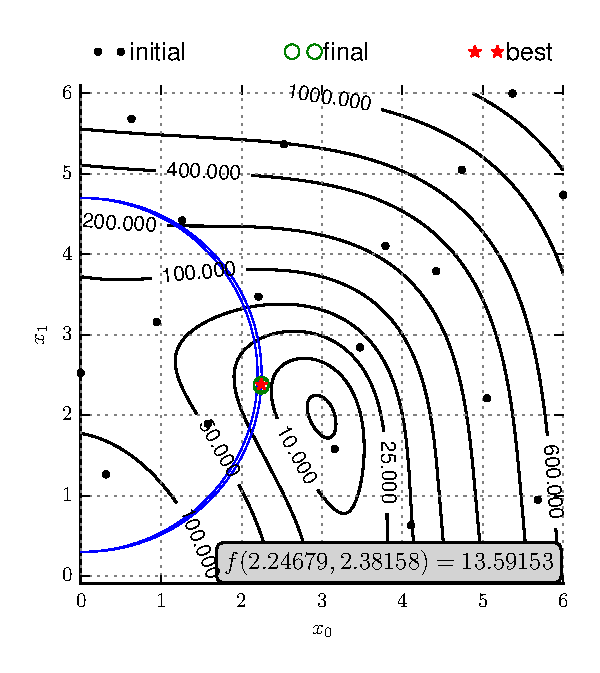
\includegraphics[scale=0.9]{./figs/res/simpleoptm3.eps}
\caption{Problem 1: Narrow crescent-shaped region with equality constraint.}
\label{fig:simple3}
\end{figure}


\emph{Problem 2} has 13 variables, 9 inequalities and is relatively easy because it involves only
quadratic terms in the objective function and has linear constraints. It corresponds to
\emph{case 1} in \citep{mich:95} and
\emph{test 3} in \citep{deb:00}
and is defined by
\OptmProbTwo
where the limits of variables are
\OptmProbTwoX


\emph{Problem 3} has 5 variables, 6 inequalities and has normal difficulty since it involves a
quadratic objective function and has quadratic constraint functions. It corresponds to
\emph{problem 83 (page 102)} in \citep{hock:81} and
\emph{test 6} in \citep{deb:00} 
and is defined by
\OptmProbThreeB
where the $c_i$ coefficients are given by
\OptmProbThreeA
and the limits of variables are
\OptmProbThreeX


\emph{Problem 4} has 5 variables, 38 inequalities and is of moderate difficulty because it involves
a large number of nonlinear constraints up to the second order. It corresponds to
\emph{{problem~85} (page 104)} in \citep{hock:81} and
\emph{test 2} in \citep{deb:00}. The objective function is defined as follows
\OptmProbFourCa
the constraints are given by
\OptmProbFourCb
and the limits of variables are
\OptmProbFourX
In addition, a number of constants and coefficients are required. The $a$ and $b$ constants are given by
\OptmProbFourD
and
\OptmProbFourE
The additional dependent variables that have to be computed in the presented order are
\OptmProbFourAB


\emph{Problem 5} has 4 variables, 5 inequalities and is of moderate difficulty because of the cubic
expressions in the objective and constraint functions. It corresponds to the design of a welded beam
firstly presented in \citep{rags:76} (see also \citep{ravi:07}) where the objective function is the
system cost. As shown in \citep{ravi:07} (page 592), after substitutions, the problem is defined by
\OptmProbFiveA
where $F=6000$, $\tau_d=13600$, $\OptmProbFiveB$. The limits of variables selected here are
\OptmProbFiveX


\emph{Problem 6} has 7 variables, 4 inequalities and is of moderate difficulty with a fourth order
term in the objective function and nonlinear constraints. It corresponds to
\emph{problem 100 (page 111)} in \citep{hock:81},
\emph{case 3} in \citep{mich:95} and 
\emph{test 5} in \citep{deb:00}.
The problem is defined by
\OptmProbSix
According to \citep{hock:81}, there are no bounds for the variables. Nonetheless, the search
space is defined as suggested in \citep{mich:95,deb:00}. Thus, the limits for variables are
\OptmProbSixX


\emph{Problem 7} has 10 variables, 8 inequalities and is also of moderate difficulty with quadratic
terms and nonlinear constraints. It corresponds to
\emph{problem 113 (page 122)} in \citep{hock:81},
\emph{case 5} in \citep{mich:95} and
\emph{test 8} in \citep{deb:00}.
The objective function for this problem is defined by
\OptmProbSevenA
As in the previous problem, there are no bounds for the variables. Thus, the following limits as in
\citep{mich:95,deb:00} are adopted
\OptmProbSevenX
The constraints for problem 7 are given by
\OptmProbSevenB


\emph{Problem 8} has 8 variables, 6 inequalities and is a difficult problem as observed in
\citep{mich:96,deb:00}. It has a linear objective function and nonlinear constraints and corresponds
to
\emph{problem 106 (page 115; heat exchanger design)} in \citep{hock:81},
\emph{case 2} in \citep{mich:95} and
\emph{test 4} in \citep{deb:00}.
The problem is defined by
\OptmProbEight
where the limits of variables are
\OptmProbEightX


\emph{Problem 9} has 5 variables, 3 equality constraints and is a very difficult problem. The
objective function is the exponential of all variables multiplied together. The equality constraints
are nonlinear (quadratic and cubic) expressions. To handle these constraints $\epsilon_h=10^{-3}$
is selected. The problem corresponds to
\emph{problem 80 (page 100)} in \citep{hock:81},
\emph{case 4} in \citep{mich:95} and
\emph{test 7} in \citep{deb:00}.
The problem is defined by
\OptmProbNine
where the limits of variables are
\OptmProbNineX


The nine problems are solved 1000 times (samples) each with ${t_{max}=500}$ iterations. After one
sample is finished, all values are initialised, the population is randomly re-created (with a
different seed), and the evolution is run all over again. The results are collected in
Table~\ref{tab:one-obj:A} alongside other input data and histograms of computed objective values. In
this table, $T_{sys}$ is the computer (system) time measured during the complete analysis of all
samples, including the $1000 \times 500$ loops. The resulting number of function evaluations
\emph{per} sample is $N_{eval}$; calling $f_i$, $g_i$, and $h_i$ at the same time counts as 1
evaluation. Below the histogram, $count$ refers to the number of feasible solutions in the final
set. The computed solutions are indicated by $X_{best}$ and the reference ones by $X_{ref.}$ and
$f_{ref}$. 


\import{./}{res-one-obj.tex}

\import{./}{res-prob2and9.tex}


In these experiments, the number of trial solutions $N_{sol}$ is fixed and calculated as
${10\,N_x}$---ten times the number of variables as in \citep{deb:00}. Sometimes more solutions are
needed and sometimes the problem could be easily solved with less; but this has not been attempted.
It is worth noting also that the number of groups ($N_{cpu}$) is selected to reduce the number of
solutions in the same group (no more than 50). When needed, the exchange time $\Delta t_{exc}$ is
simply set equal to $\Delta t_{exc} = t_f / 10$.

An important parameter is the differential evolution coefficient $C_{DE}$ (indicated in all tables
with results). By default, this value is fixed as ${C_{DE}=0.8}$. Later on, the value is changed for
some multi and many objective tests whenever the performance can be improved.

The code works really well for problems 1 to 7 with the standard deviation $f_{dev}$ being very
small. This means that every time the code is run the same solution is obtained; except by 9 out of
1000 non optimal results in problem 2 (to be discussed soon next). In problem 7, the results are not
bad; but there is a small standard deviation and a slightly larger spread in the histogram. In
problems 1 to 7, minimum values ($f_{min}$) close to the reference ones are obtained. Problem 8 is
more difficult to be solved and requires longer evolution times. 

In problem 2, the failure happens because the optimal solution is actually at the boundaries of the
search space. In this case, the solution reaches the maximum limit. This can be improved by
employing a larger search space and adding extra $g_i$ constraints as follows
\OptmProbTwoFix
Thus, the number of constraints increases to $N_f=35$. The limits of variables defining the
search space can now be specified as
\OptmProbTwoXfix
Note that this is a natural way to define the constrained optimisation problem. The convenience of
the \emph{box approach} where the variables are always limited is apparent in reducing the number of
constraint functions. The problem is run again and the minimum is always obtained. The results are
listed in Table~\ref{tab:prob2and9} and are quite good now.

Problem 9 requires longer times and is actually a challenging one. The reason this problem is
difficult is the five multiplications $x_0\,x_1\,x_2\,x_3\,x_4$ inside the exponential function in
\eqname~(\ref{eqn:optmprob:nine}) and the `narrow' equality constraints. This means that the sign of
pairs $x_i\,x_j$ ($i \neq j$) can vary freely causing problems to the differential evolution
operator. Moreover, the equality constraint makes it harder to find feasible solutions because the
search space is largely reduced to fall within the band specified by $\epsilon_h$. Problem 9 is run
again with 7000 iterations as in \citep{deb:00}. The results are collected in
Table~\ref{tab:prob2and9} where it can bee seen the minimum is found with higher frequency. By
tweaking the parameters and extending the number of iterations the results would improve; but this
has not been pursued.



\section{Test cases: unconstrained two-objective}
\label{sec:exMulti}

Multi objective optimisation problems may be more challenging than single objective problems at
times, especially if the whole extent of the Pareto-optimal front is sought and the search space
involves local optima. Now, two quantities are required in order to assess the accuracy and quality
of results: (1) a measure of how well points are located close to the optimal front ($E$); and (2) a
measure of the spread of points along the optimal front ($L$). In this paper, the accuracy is
assessed by an error measure given by the root mean square error between the numerical and
analytical solutions. The spread is calculated by summing the distance of points along the optimal
front (two-objective problems only).

In this section, unconstrained problems with two objective functions $f_0(\vx)$ and $f_1(\vx)$ are
considered; six problems are studied. Five of them, named \emph{ZDTi} were proposed in
\citep{zit:00}. These problems include concave and convex curves in the $(f_0,f_1)$ space and
situations of multiple local minima. The interesting problem \emph{FON} \citep{fonseca:95} in the
form presented in \citep{deb:01a} is also studied.

Except for \emph{FON}, in the problems presented in this section, $C_{DE}$ has been reduced to
$C_{DE}=0.1$ because it was found that this value produces better results (accuracy and spread).
With $C_{DE}=0.8$, the results are not bad though; however \emph{ZDT4} requires more iterations due
to the local fronts.



\emph{Problem ZDT1} has a convex Pareto-optimal front and is relatively easy to solve. It is defined
by
\ZDTone
where the limits of variables are
\ZDToneX
$N_x=30$ is selected and the optimal front is expressed by
\ZDToneFront
for which a line integral in ${0 \leq f_0 \leq 1}$ produces an arc length of ${\ZDToneArcLen}$.


\emph{Problem ZDT2} has a concave Pareto-optimal front and is easy to solve as well. It is defined
by
\ZDTtwo
where the limits of variables are
\ZDTtwoX
$N_x=30$ is selected and the optimal front is expressed by
\ZDTtwoFront
for which a line integral in ${0 \leq f_0 \leq 1}$ also produces an arc length of ${\ZDTtwoArcLen}$.


\emph{Problem ZDT3} has a number of disconnected Pareto-optimal fronts but is not difficult to
solve. It is defined by
\ZDTthree
where the limits of variables are
\ZDTthreeX
$N_x=30$ is selected and the optimal front is expressed by
\ZDTthreeFront
The arc length of the Pareto front in the $(f_0,f_1)$ plane has to be computed in five steps (a to
e) by performing line integrals along the following ranges
\ZDTthreeFrontRanges
The above numbers were computed by means of solving a simple nonlinear problem for the local minima
on the curve $f_1(f_0)$ using Newton's method. The first value is chosen equal to
$10^{-7}$ though. The arc length is the sum of five integrals (numerically computed) resulting in
$\ZDTthreeArcLen$.


\emph{Problem ZDT4} has a convex Pareto-optimal front and is a difficult one. It presents
challenges to the solver because there are many local optimal fronts. It is defined by
\ZDTfour
where the limits of variables are
\ZDTfourX
$N_x=10$ is selected and the optimal front is defined by
\ZDTfourFront
for which a line integral in ${0 \leq f_0 \leq 1}$ produces an arc length of ${\ZDTfourArcLen}$
as well.


\emph{Problem ZDT6} has a concave Pareto-optimal front and is of moderate difficulty. Actually
\goga~solves this problem very well. The difficulty in this problem is related to the non-uniformity
of the Pareto-optimal region. It is defined by
\ZDTsix
where the limits of variables are
\ZDTsixX
$N_x=10$ is selected and the optimal front is defined by
\ZDTsixFront
In this problem, the curve representing the Pareto-optimal front in the $(f_0,f_1)$ plane is limited
to the left by a point $(f_0^{\star},f_1^{\star})$. This point can be found by using
\ZDTsixXstar
in \eqname~(\ref{eqn:ZDTsix}) to compute $f_0^{\star}=0.280775$ which can then be inserted into
\eqname~(\ref{eqn:ZDTsix:front}) to calculate $f_1^{\star}=0.921165$. The arc length can now be
computed by a line integral in $f_0^{\star} \leq f_0 \leq 1$ resulting in $\ZDTsixArcLen$.


\emph{Problem FON} has a somewhat concave Pareto-optimal front in part of the domain (except near
$f_0=0$ or $f_0=1$) and has moderate difficulty. It is defined by
\FON
where the limits of variables are
\FONx
$N_x=10$ is selected and the optimal front is defined by
\FONfront
for which a line integral in $0 \leq f_0 \leq 0.98$ produces an arc length of $\FONarcLen$.


The results are discussed next. Again, 1000 samples are run in order to compute some statistics on
the error $E$ and spread $L$. Each sample is executed with $t_f=500$ iterations and the number of
solutions is ${N_{sol}=10\,N_x}$, as before. The number of groups $N_{cpu}$ is equal to 6 for the
problems with $N_{sol}=30$ and equal to 2 for problems with $N_{sol}=10$. The exchange time is
$T_{exc}=t_f/10$.

For each sample, the following root mean square error $E$ is computed
\begin{equation}
E = \sqrt{ \frac{1}{n} \sum_{i=0}^{n-1} \left[ f_1^{i} - f_1^{ana}(f_0^{i}) \right]^2 }
\end{equation}
where $f_0^i$ is the numerical solution corresponding to $\vx_i$ and $n$ is the number of solutions
(points) that are feasible and non-dominated at the best front ($\phi_i=0$).

The spread is computed by adding the Euclidean distance between successive points along the optimal
front; from left to right in a $(f_0,f_1)$ graph. This measure is then normalised by the reference
arc length $L_{ref}$ determined analytically. The definition of $L$ is thus
\begin{equation}
    L = \frac{1}{L_{ref}} \sum_{\substack{1 \leq j < n \\ 0 \leq i < n-1}} \sqrt{\left(f_0^j-f_0^i\right)^2 + \left(f_1^j-f_1^i\right)^2}
\end{equation}
where $n$ indicates the number of \emph{feasible} solutions on the optimal front with $\phi_i=0$.
Therefore, contrary to the error measure, the spread is better if closer to 1. Note that the
above measure does not account for how equally spaced points are.

Table~\ref{tab:two-obj:A} collects the results from all 1000 samples where it can be observed that
the performance is very good with the error achieving the machine precision 0 for four tests. A good
spread is also observed in all problems. Finally, the repeatability behaviour is also excellent with
a very small standard deviation both in terms of accuracy ($E$) and spread ($L$). Plots of
Pareto-optimal fronts for the six problems are presented in \figname~\ref{fig:two-obj} corresponding
to one (any) sample. 

\begin{figure*} \centering
\subcaptionbox{ZDT1\label{fig:ZDT1}}[0.49\linewidth]{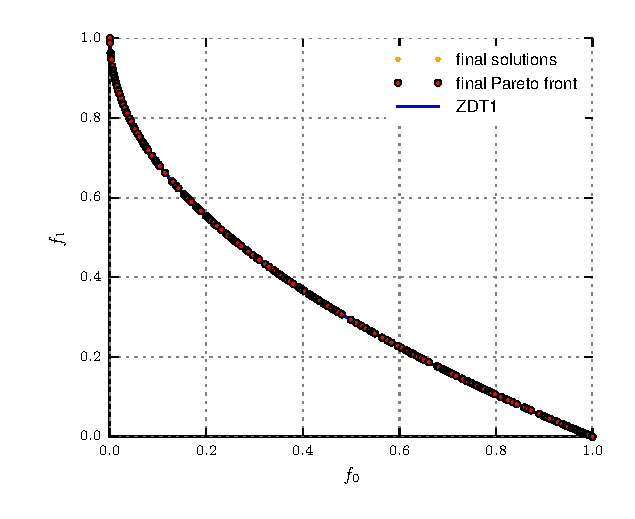
\includegraphics[width=0.45\linewidth]{./figs/res/ZDT1.eps}}
\subcaptionbox{ZDT2\label{fig:ZDT2}}[0.49\linewidth]{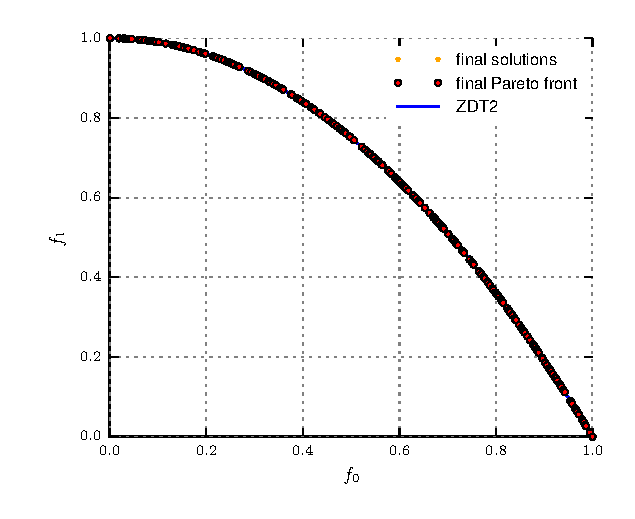
\includegraphics[width=0.45\linewidth]{./figs/res/ZDT2.eps}}
\subcaptionbox{ZDT3\label{fig:ZDT3}}[0.49\linewidth]{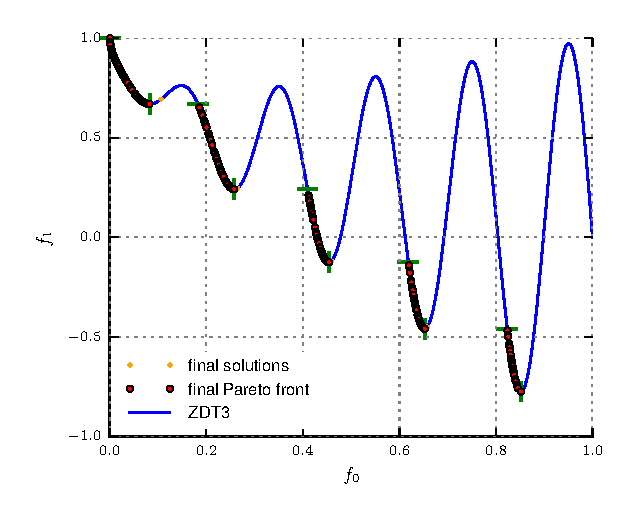
\includegraphics[width=0.45\linewidth]{./figs/res/ZDT3.eps}}
\subcaptionbox{ZDT4\label{fig:ZDT4}}[0.49\linewidth]{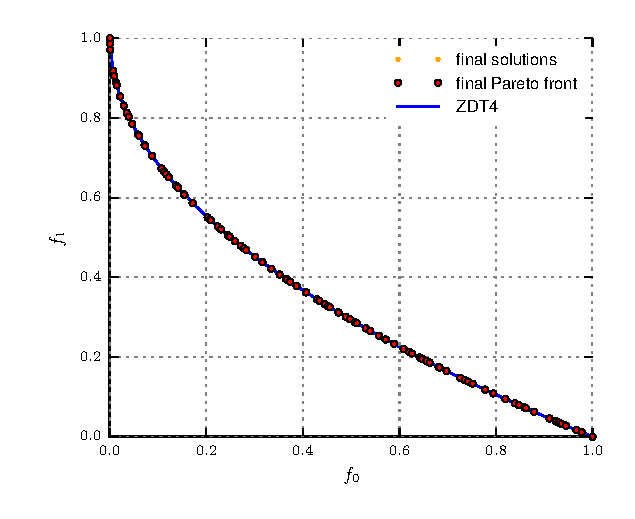
\includegraphics[width=0.45\linewidth]{./figs/res/ZDT4.eps}}
\subcaptionbox{ZDT6\label{fig:ZDT6}}[0.49\linewidth]{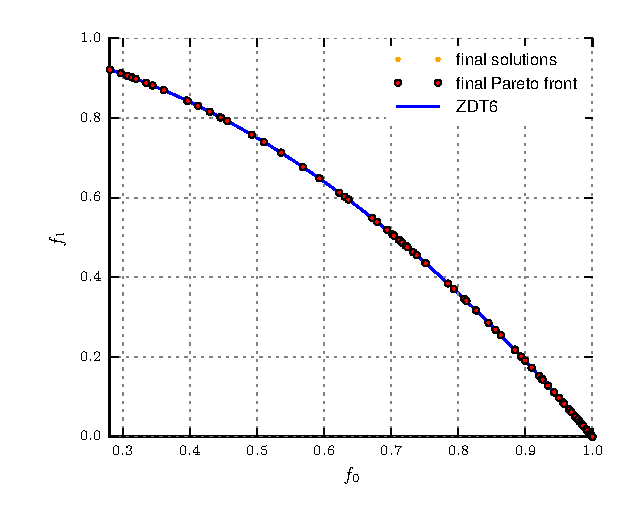
\includegraphics[width=0.45\linewidth]{./figs/res/ZDT6.eps}}
\subcaptionbox{FON \label{fig:FON} }[0.49\linewidth]{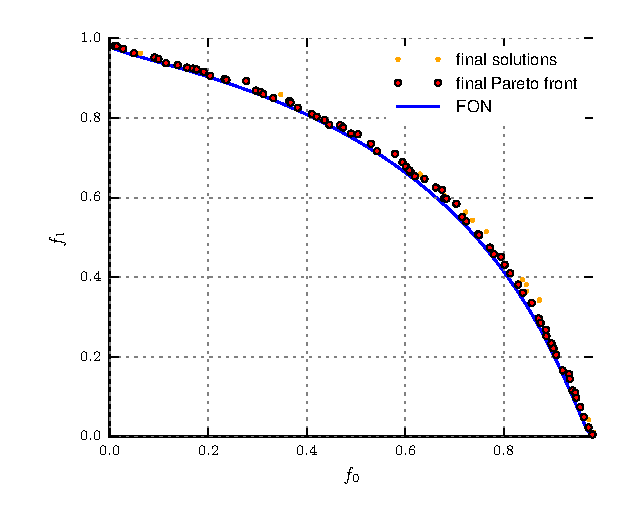
\includegraphics[width=0.45\linewidth]{./figs/res/FON.eps}}
\caption{Unconstrained two-objective problems.}% (a) ZDT1. (b) ZDT2. (c) ZDT3. (d) ZDT4. (e) ZDT6. (f) FON.}
\label{fig:two-obj}
\end{figure*}

\import{./}{res-two-obj.tex}



\section{Test cases: constrained two objective}
\label{sec:twoObj}

The next set of tests deals with constrained two objective optimisation problems. In this case, the
accuracy is assessed by computing a scalar function $\psi(f_0,f_1,f_2,\ldots)=0$ expressing the
optimal front with the numerical results. A root mean square error is thus computed by means of
\begin{equation}
E = \sqrt{ \frac{1}{n} \left[ \sum_{i=0}^{n-1} \psi(f_0^i,f_1^i,f_2^i,\ldots)^2 \right] }
\end{equation}
where $f_j^i$ is the numerical solution $i$ for objective function $j$ and $n$ indicates the number
of feasible solutions on the optimal front with $\phi_i=0$.

A series of problems presented in \citep{deb:01a} are considered. These problems are symbolised by
\emph{CTPi} and include some with local minima and nonuniform distribution of points on the
Pareto-optimal fronts. The problem \emph{TNK} from \citep{tanaka:95} is studied as well.

Nine problems are considered as described below. The number of solutions for these problems is
chosen as $N_{sol}=120$ in order to better draw the optimal front. The differential evolution
coefficient $C_{DE}$ is set equal to $C_{DE}=0.1$ because this value seemed to give better results
when solving the problems in this section. A statistical analysis is presented just after all
problems are described.


\emph{Problem TNK} \citep{tanaka:95} has two constraints and a discontinuous optimal front. $N_x=2$
and the problem is defined by
\TNK
where the limits of variables are
\TNKx
The results are plotted in \figname~\ref{fig:TNK} where it can be seen a good
response: accurate and spread. In addition, all solutions satisfy the constraints. 


\begin{figure} \centering
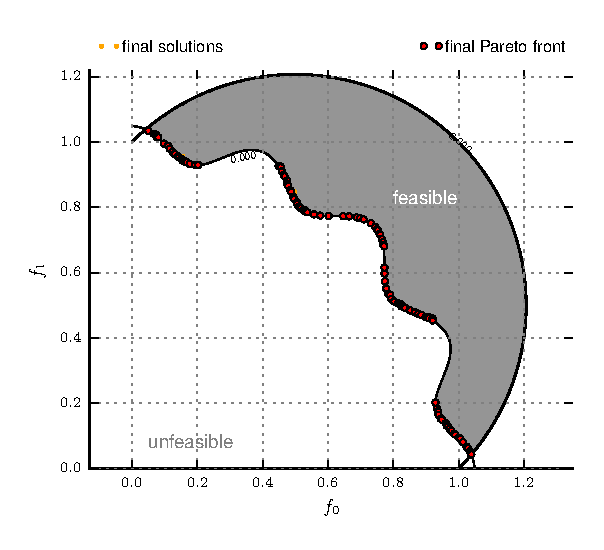
\includegraphics[width=\linewidth]{./figs/res/TNK.eps}
\caption{Constrained two objective test: TNK.}
\label{fig:TNK}
\end{figure}


The next \emph{CTPi} problems are all defined with $N_x=10$ and two groups ($N_{cpu}=2$). The limits
of variables for all of them are
\CTPx


\emph{Problem CTP1} \citep{deb:01a}, as considered in this work, has two constraints and is defined
by
\CTPone
where the following auxiliary coefficients are selected
\CTPoneC
Good results are obtained as illustrated in \figname~\ref{fig:CTP1}---a statistical analysis is
given shortly.


\emph{Problems CTP2-CTP7} \citep{deb:01a} have one constraint and, in this work, are all defined by
the following expressions
\CTPi
where $a$, $b$, $c$, $d$, $e$ and $\theta$ are auxiliary coefficients that help to design many
combinations. The selected values are listed in Table~\ref{tab:CTP2-7}.


% table
\CTPtwoSeven


\emph{Problem CTP2} has a number of narrow discontinuous Pareto-optimal fronts as illustrated in
\figname~\ref{fig:CTP2}. The presented code can obtain satisfactory results every time it is
run.

\emph{Problem CTP3} is more challenging because the optimal front reduces to a set of single points
(\figname~\ref{fig:CTP3}).

\emph{Problem CTP4} (\figname~\ref{fig:CTP4}) is also more challenging because the `path' available for
points to move towards the best front is very narrow. The proposed code is able to obtain some
reasonable results.

\emph{Problem CTP5} is similar to Problem CTP3 but has a nonuniform distribution of points along the
optimal front. The results are plotted in \figname~\ref{fig:CTP5} and the response is similar to
CTP3 where the points do approach the optimal front with good spread.

\emph{Problem CTP6} has bands defining feasible and infeasible regions; hence additional problems would
arise if the solver was not able to properly handle and `jump over' constraints.
\figname~\ref{fig:CTP6} show the results where the optimal front lies along the constraint
line.

\emph{Problem CTP7} (\figname~\ref{fig:CTP7}) has also multiple infeasible regions. The Pareto-optimal
front is discontinuous and follows a straight line defined by $f_1=1-f_0$.


\emph{Problem CTP8} \citep{deb:01a} is now introduced. This problem is similar to the previous CTP
ones; however two constraints using the same generator are considered. For the sake of clarity, the
equations are written below
\CTPeight
where $c_0$, $f_0$ and $f_1$ are the same as in \eqname~(\ref{eqn:CTPi}). The auxiliary coefficients are
\CTPeightC
and
\CTPeightCx
The results are presented in \fignames~\ref{fig:ct-two-objA} and \ref{fig:ct-two-objB} where it can
be observed that there are `islands' of feasible and infeasible regions and that the optimal front
is discontinuous. The proposed code seems to also work well in this case.

\begin{figure*} \centering
\subcaptionbox{CTP1\label{fig:CTP1}}[0.49\linewidth]{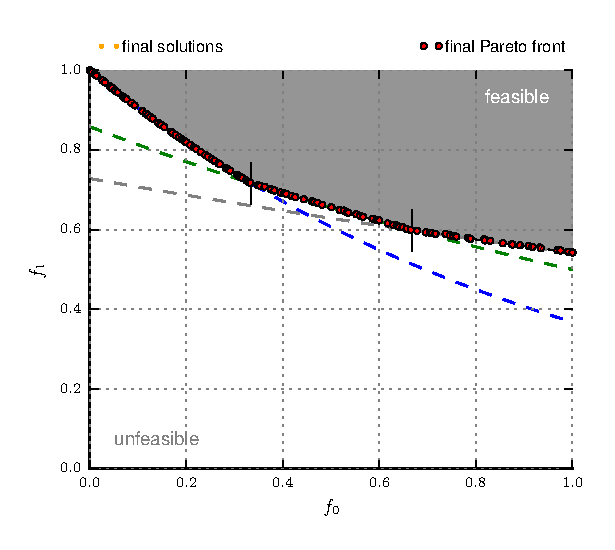
\includegraphics[width=0.42\linewidth]{./figs/res/CTP1.eps}}
\subcaptionbox{CTP2\label{fig:CTP2}}[0.49\linewidth]{\includegraphics[width=0.42\linewidth]{./figs/res/CTP2.eps}}
\subcaptionbox{CTP3\label{fig:CTP3}}[0.49\linewidth]{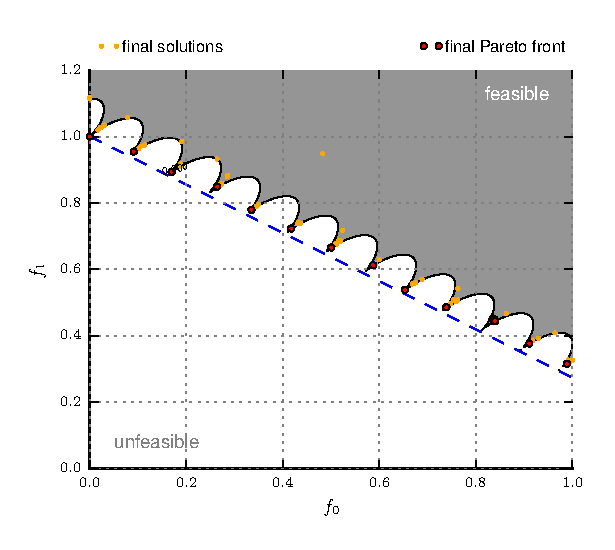
\includegraphics[width=0.42\linewidth]{./figs/res/CTP3.eps}}
\subcaptionbox{CTP4\label{fig:CTP4}}[0.49\linewidth]{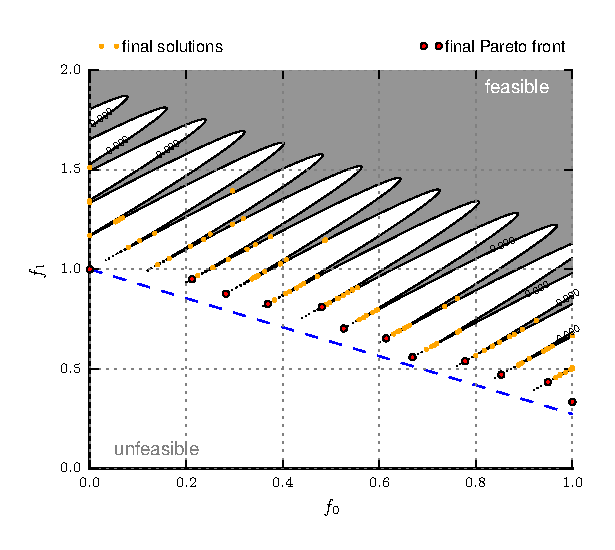
\includegraphics[width=0.42\linewidth]{./figs/res/CTP4.eps}}
\subcaptionbox{CTP5\label{fig:CTP5}}[0.49\linewidth]{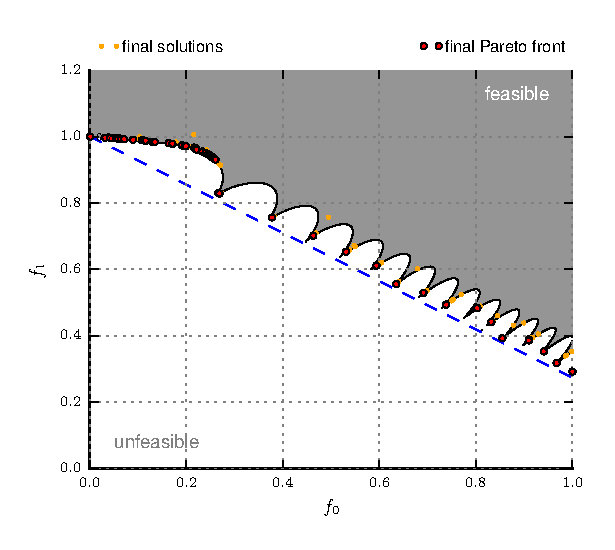
\includegraphics[width=0.42\linewidth]{./figs/res/CTP5.eps}}
\subcaptionbox{CTP6\label{fig:CTP6}}[0.49\linewidth]{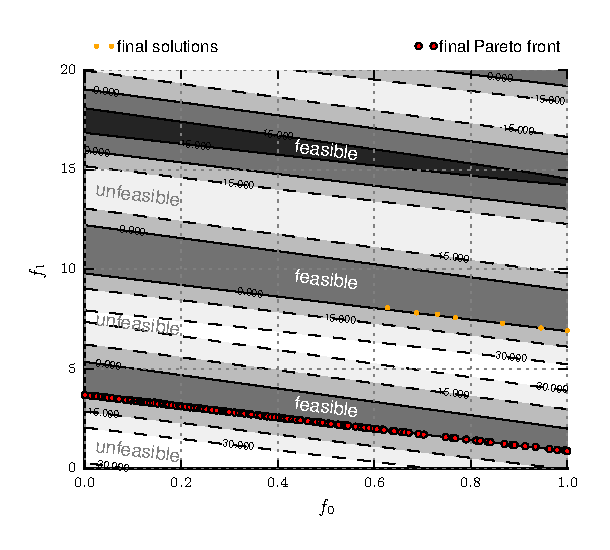
\includegraphics[width=0.42\linewidth]{./figs/res/CTP6.eps}}
\caption{Constrained two-objective problems.}% (a) CTP1. (b) CTP2. (c) CTP3. (d) CTP4. (e) CTP5. (f) CTP6.}
\label{fig:ct-two-objA}
\end{figure*}

\begin{figure*} \centering
\subcaptionbox{CTP7\label{fig:CTP7}}[0.49\linewidth]{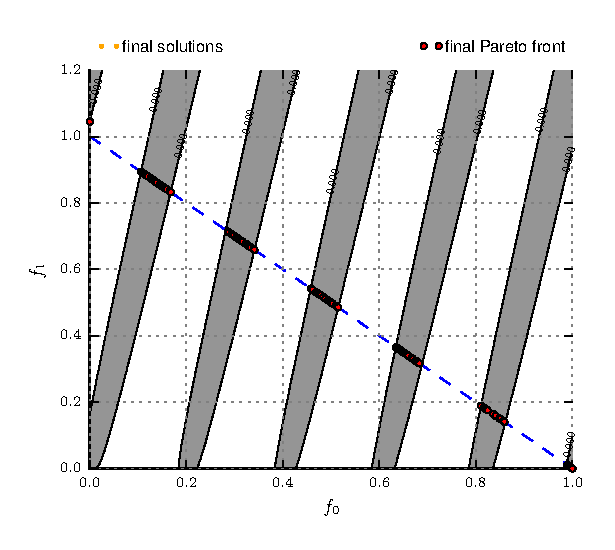
\includegraphics[width=0.42\linewidth]{./figs/res/CTP7.eps}}
\subcaptionbox{CTP8\label{fig:CTP8}}[0.49\linewidth]{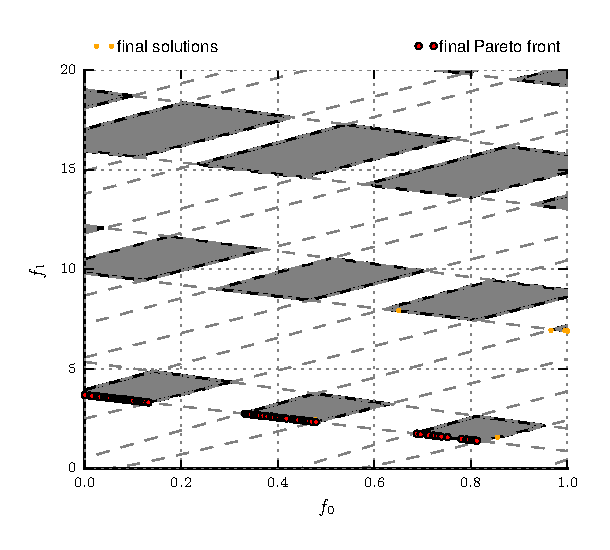
\includegraphics[width=0.42\linewidth]{./figs/res/CTP8.eps}}
\caption{Constrained two-objective problems (contd.).}% (a) CTP7. (b) CTP8.}
\label{fig:ct-two-objB}
\end{figure*}

Each problem is run 1000 times (samples) generating data for the statistical analysis. Once again,
$T_{sys}$ is the computer (system) time spent in running \emph{all 1000 samples} of one particular
problem; hence considering the $1000 \times 500$ loops.

The statistics with respect to error are presented in Table~\ref{tab:ct-two-obj:A}. It can be
observed that the accuracy is reasonable (small $E$) and the repeatability characteristics are quite
good for all tests. The spread has been also observed in several runs---every time TNK or CTPi are
run, \fignames~\ref{fig:TNK} and \ref{fig:CTP1}-\ref{fig:CTP8} exhibit similar results.

\import{./}{res-ct-two-obj.tex}



\section{Test cases: three objective}
\label{sec:threeObj}

Nine three-objective optimisation problems are studied in this section. Eight tests are
unconstrained (except for the limits on $\vx$) and one has one constraint. As before, the number of
iterations is ${t_{max}=500}$. The number of trial solutions is set to ${N_{sol}=200}$ for all tests
in order to better depict the optimal Pareto front in the 3D space defined by ${(f_0,f_1,f_2)}$.

The set of tests introduced in \citep{deb:05} are considered. These tests are known as \emph{DTZLi}.
In addition, the convex version of \emph{DTZL2} presented in \citep{deb:14, jain:14} is solved. This
version is named here \emph{DTZL2x}. A constraint expression is added to \emph{DTZL2} and the
resulting test named \emph{DTZL2c}. Finally, a modification to \emph{DTLZi} is applied by using the
expressions of a superquadric---the resulting tests are named here as \emph{SUQ1} and \emph{SUQ2}.
In all problems, the variables are limited by
\DTLZx


\emph{Problem DTZL1} has 7 variables and is defined by
\DTLZone
The optimal Pareto front is a flat surface described by
\DTLZoneAna
The results of one run are illustrated in \fignames~\ref{fig:DTLZ1_A} and \ref{fig:DTLZ1_B} where
it can be seen that the trial solutions (spheres) are close to the optimal front indicated by the
plane. A table is presented shortly with a statistical analysis.



\emph{Problem DTZL2} has 12 variables and is defined by
\DTLZtwo
The optimal Pareto front is the surface of a sphere described by
\DTLZtwoAna
The solutions are illustrated in \figname~\ref{fig:DTLZ2_A} and \ref{fig:DTLZ2_B} and also allow
to conclude that the results are reasonable.


\emph{Problem DTLZ3} has 12 variables, is similar to the previous problem; but is more difficult
because it has a number of local fronts parallel to the global one. The problem is defined by
\DTLZthree
where the optimal front is also the surface of a sphere as in DTLZ2. The results are very similar
to the ones from DTLZ2.


\emph{Problem DTLZ4} has 12 variables and is similar to DTLZ2; however with a bias in the search
space that could cause solutions to be concentrated at planes normal to the coordinates axes. The
problem is defined by
\DTLZfour
with $\alpha=100$ and the optimal front is the surface of a sphere as in DTL2. The results are also
similar to the ones from DTLZ2.


\emph{Problem DTLZ2x} has 12 variables and is a convex version to DTLZ2---an exact convex
counterpart is given in SUQ1 below. The problem is defined by
\DTLZtwox
Note the exponents 4 and 2 that basically modify DTLZ2. The optimal Pareto front is described by
\DTLZtwoxAna
and the results are illustrated in \figname~\ref{fig:DTLZ2x_A} and \ref{fig:DTLZ2x_B} where a
good convergence can be observed with the points reaching the optimal front.


\emph{Problem DTLZ2c} is the same as DTLZ2 with the addition of one inequality constraint function.
This function ($g_0(\vx)$) defines a cone in the $f_i$ space that is aligned with its diagonal. The
constraint is defined by
\DTLZtwoc
where $\alpha$ equals half the cone's opening angle. Here, $\alpha=15$ has been selected. In this
way, the feasible solutions must lie on a circular patch of the optimal front. The results are
illustrated in \fignames~\ref{fig:DTLZ2c_A} and \ref{fig:DTLZ2c_B}.




\emph{Problems SUQi}: A superquadric version of DTLZ2 is now introduced. The expressions in
\ref{eqn:DTLZ2} are used, except that the sine and cosine functions are replaced by the following
functions
\begin{equation}
    \sinX{(w; m)} = \sign{(\sin{w})} \, |\sin{w}|^m
\end{equation}
and
\begin{equation}
    \cosX{(w; m)} = \sign{(\cos{w})} \, |\cos{w}|^m
\end{equation}
respectively. In this way, the \emph{SUQi} problems are defined by
\SUQi
where $a$, $b$ and $c$ are the coefficients of the superquadric.
The error related to the Pareto-optimal front is then
\SUQiAna
The above expressions are quite versatile because they can produce concave, convex and many kinds of
twisted surfaces in the space of objective values. Views of the Pareto-optimal fronts and numerical
results are shown in \fignames~\ref{fig:SUQ1_A} and \ref{fig:SUQ1_B} for SUQ1 and in
\fignames~\ref{fig:SUQ2_A} and \ref{fig:SUQ2_B} for SUQ2 where it can be seen that the points
(small spheres) approach the optimal front.



\begin{figure*} \centering
\subcaptionbox{DTLZ1  (view 1)\label{fig:DTLZ1_A} }[0.49\linewidth]{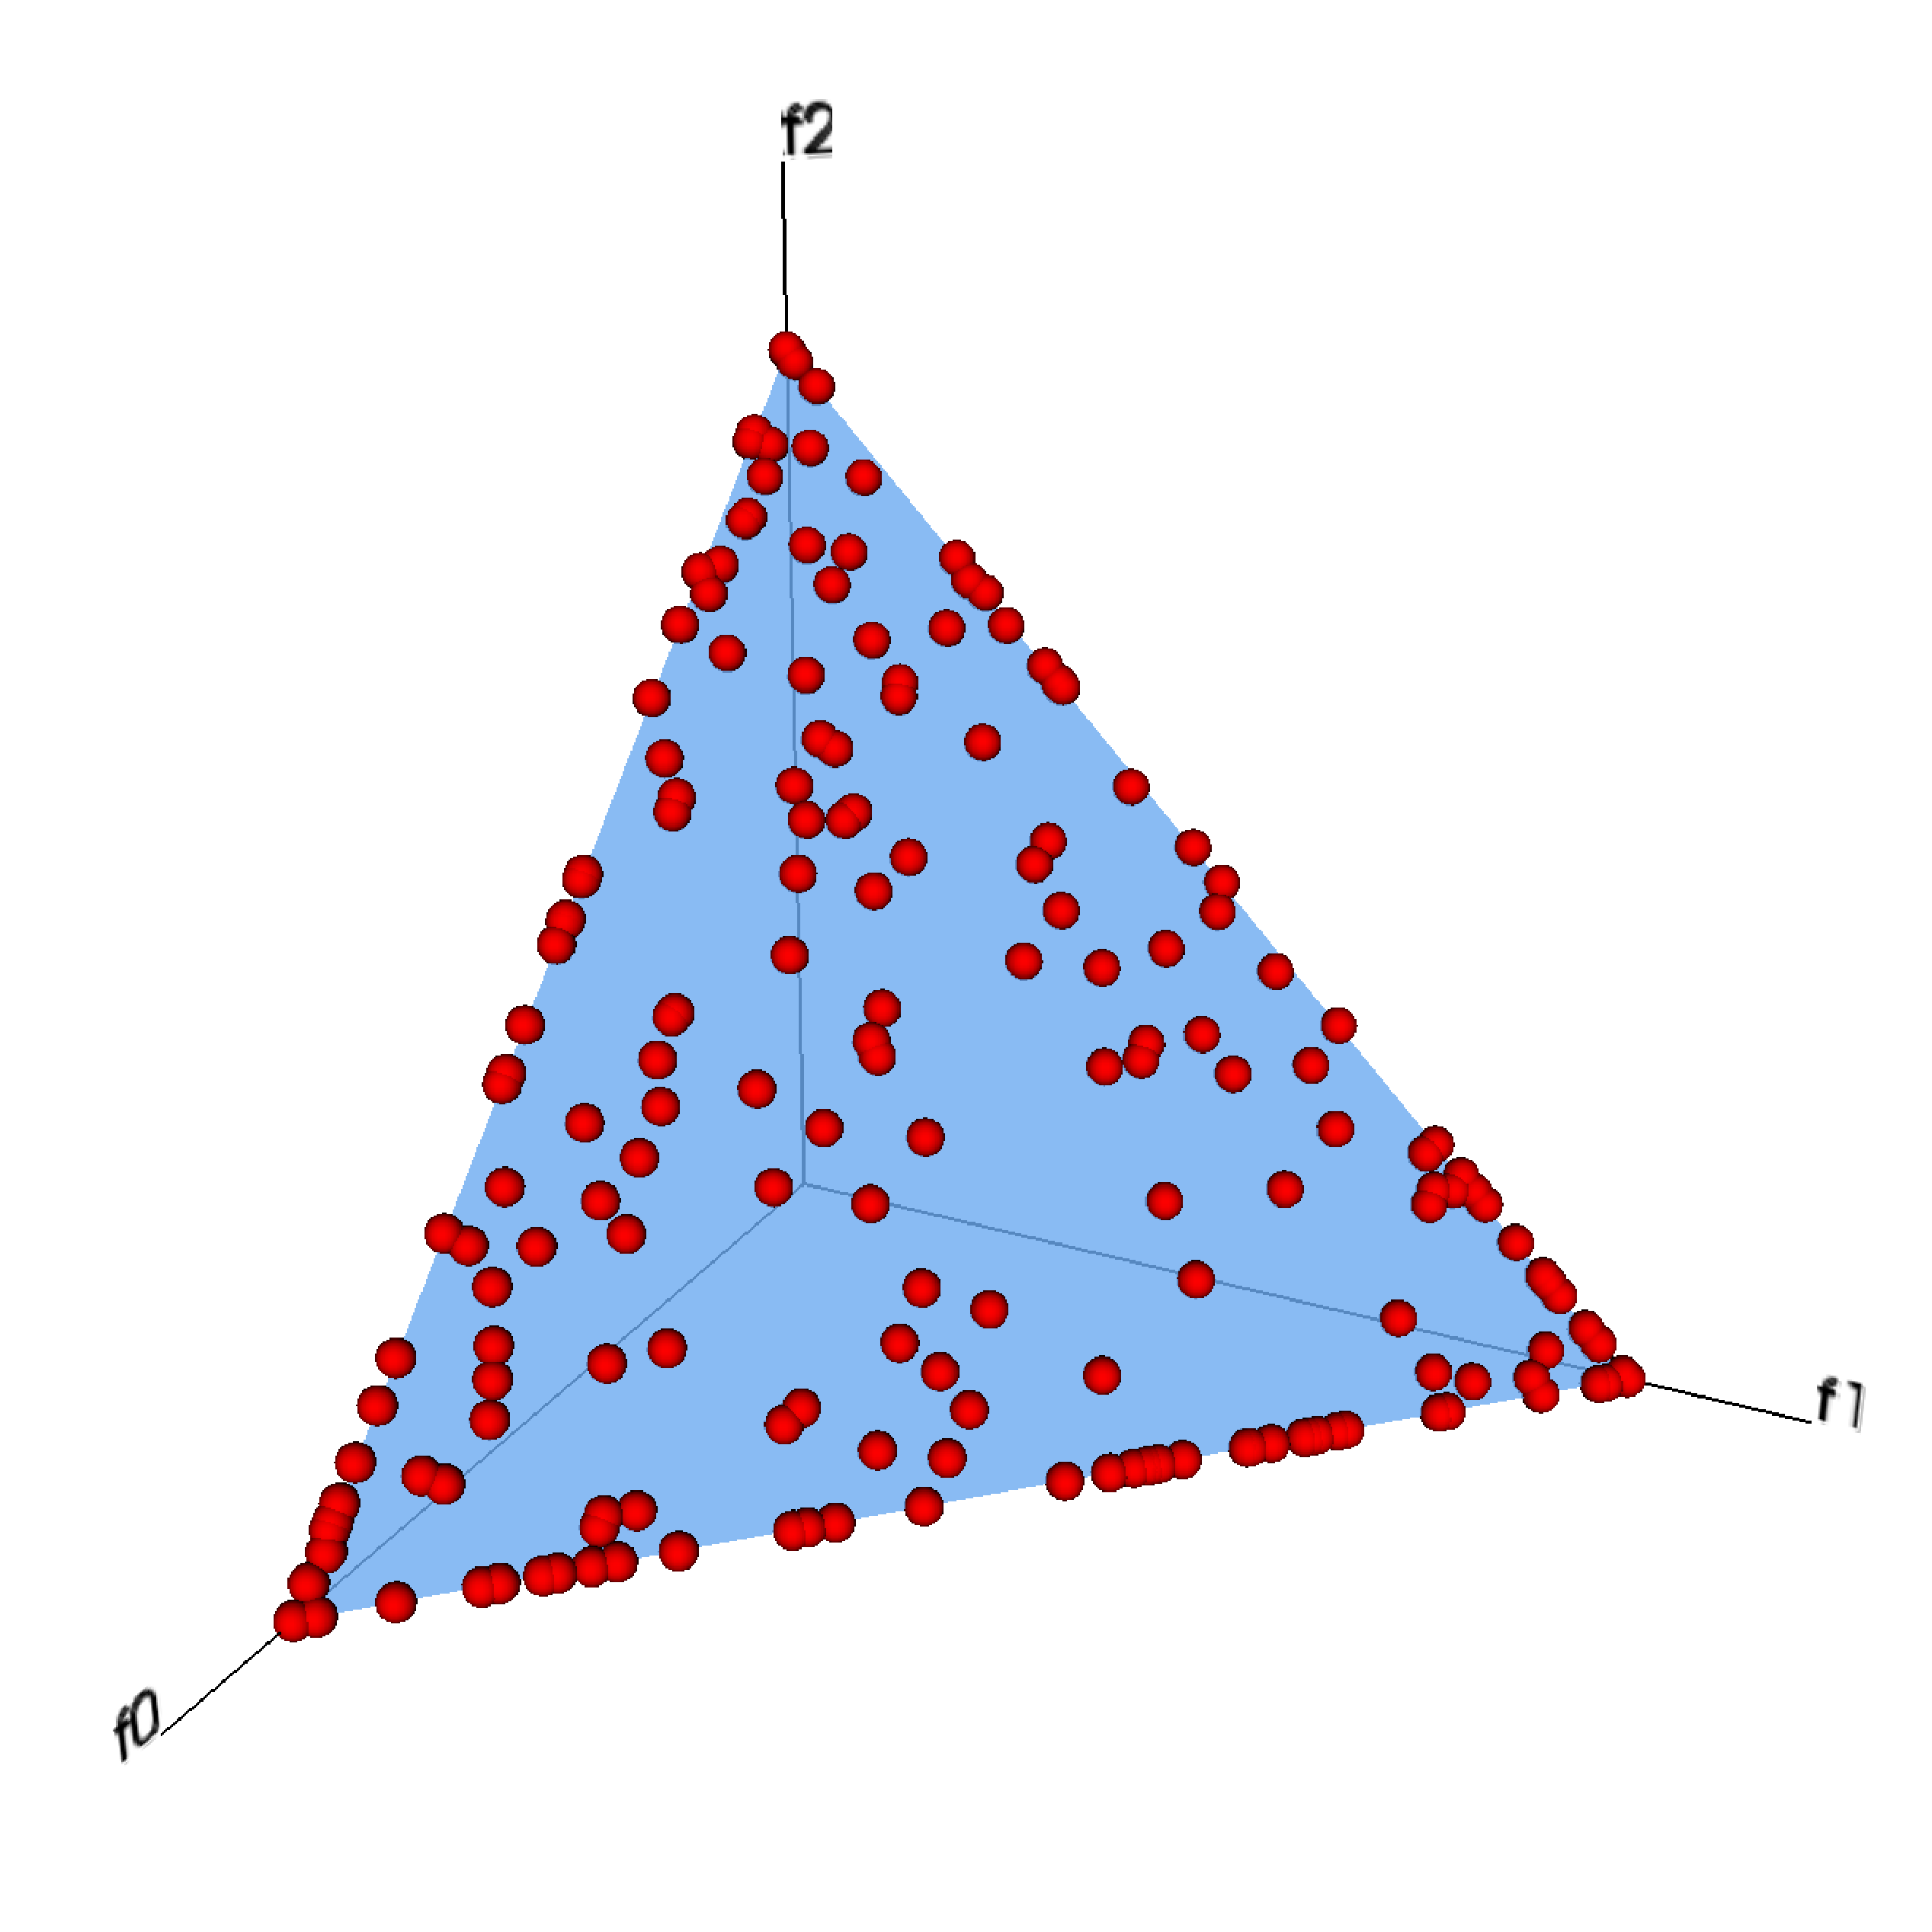
\includegraphics[width=0.38\linewidth]{./figs/res/vtk_DTLZ1_A.eps}}
\subcaptionbox{DTLZ1  (view 2)\label{fig:DTLZ1_B} }[0.49\linewidth]{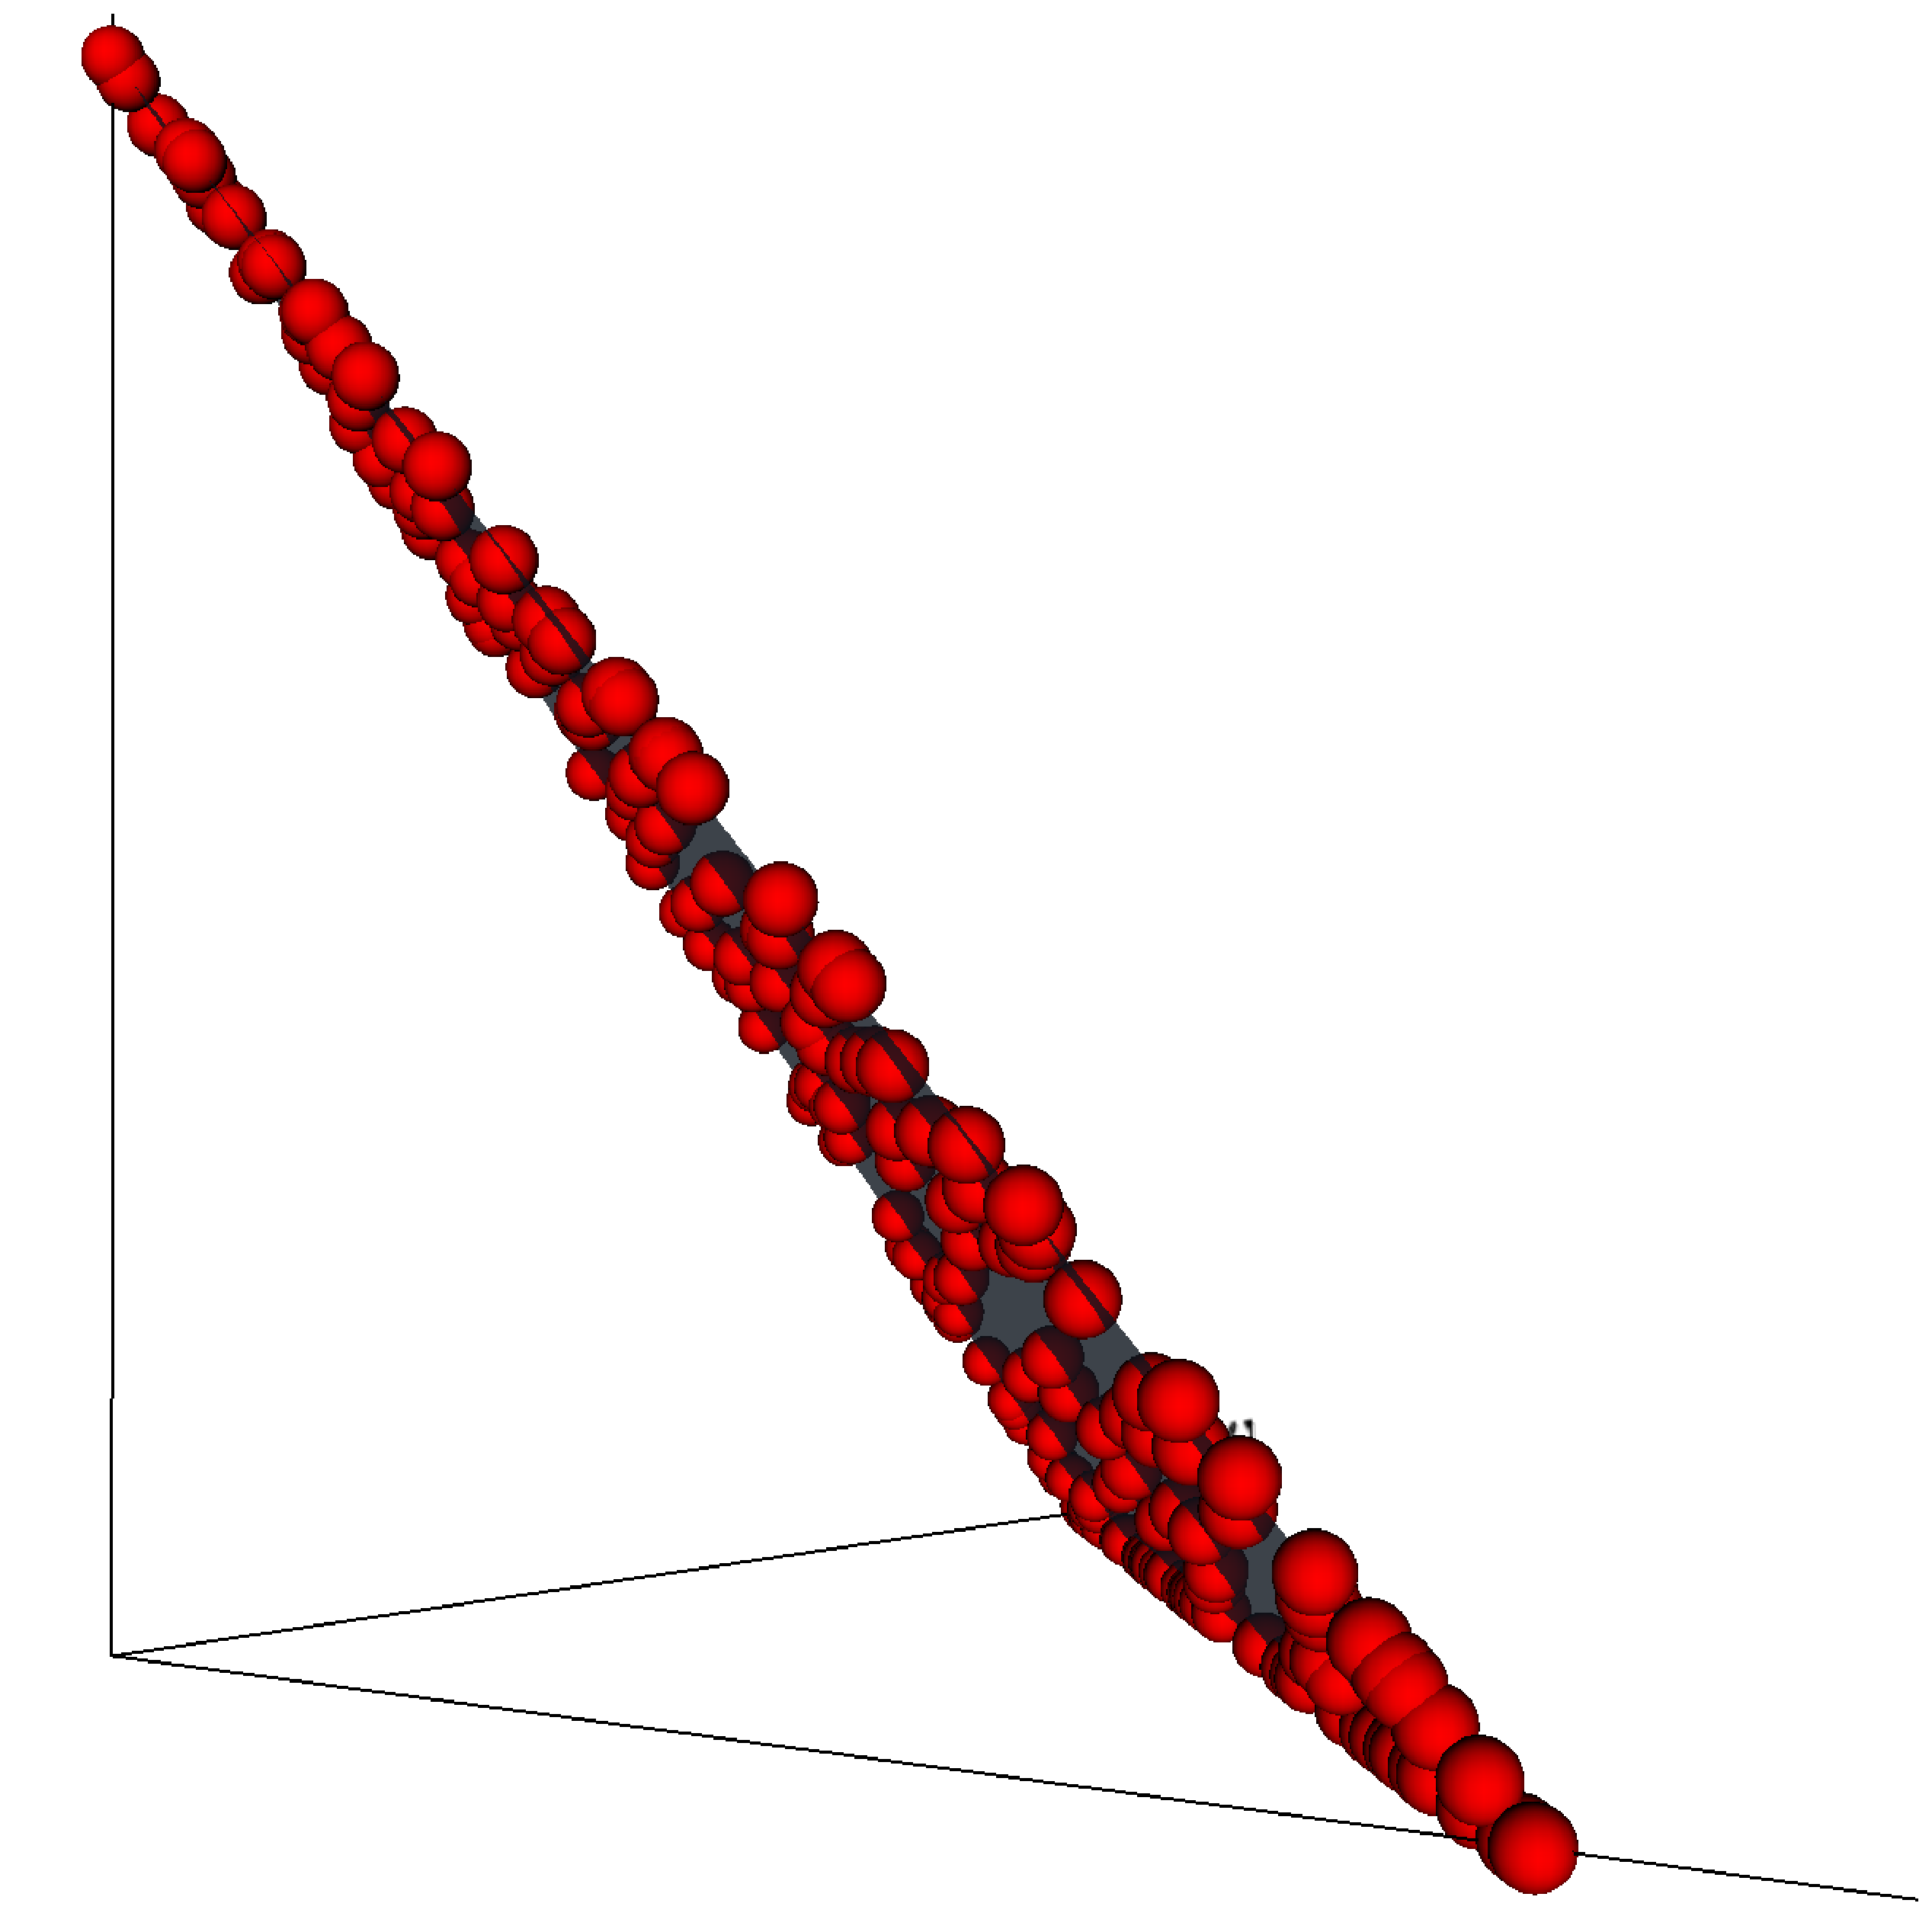
\includegraphics[width=0.36\linewidth]{./figs/res/vtk_DTLZ1_B.eps}}
\subcaptionbox{DTLZ2  (view 1)\label{fig:DTLZ2_A} }[0.49\linewidth]{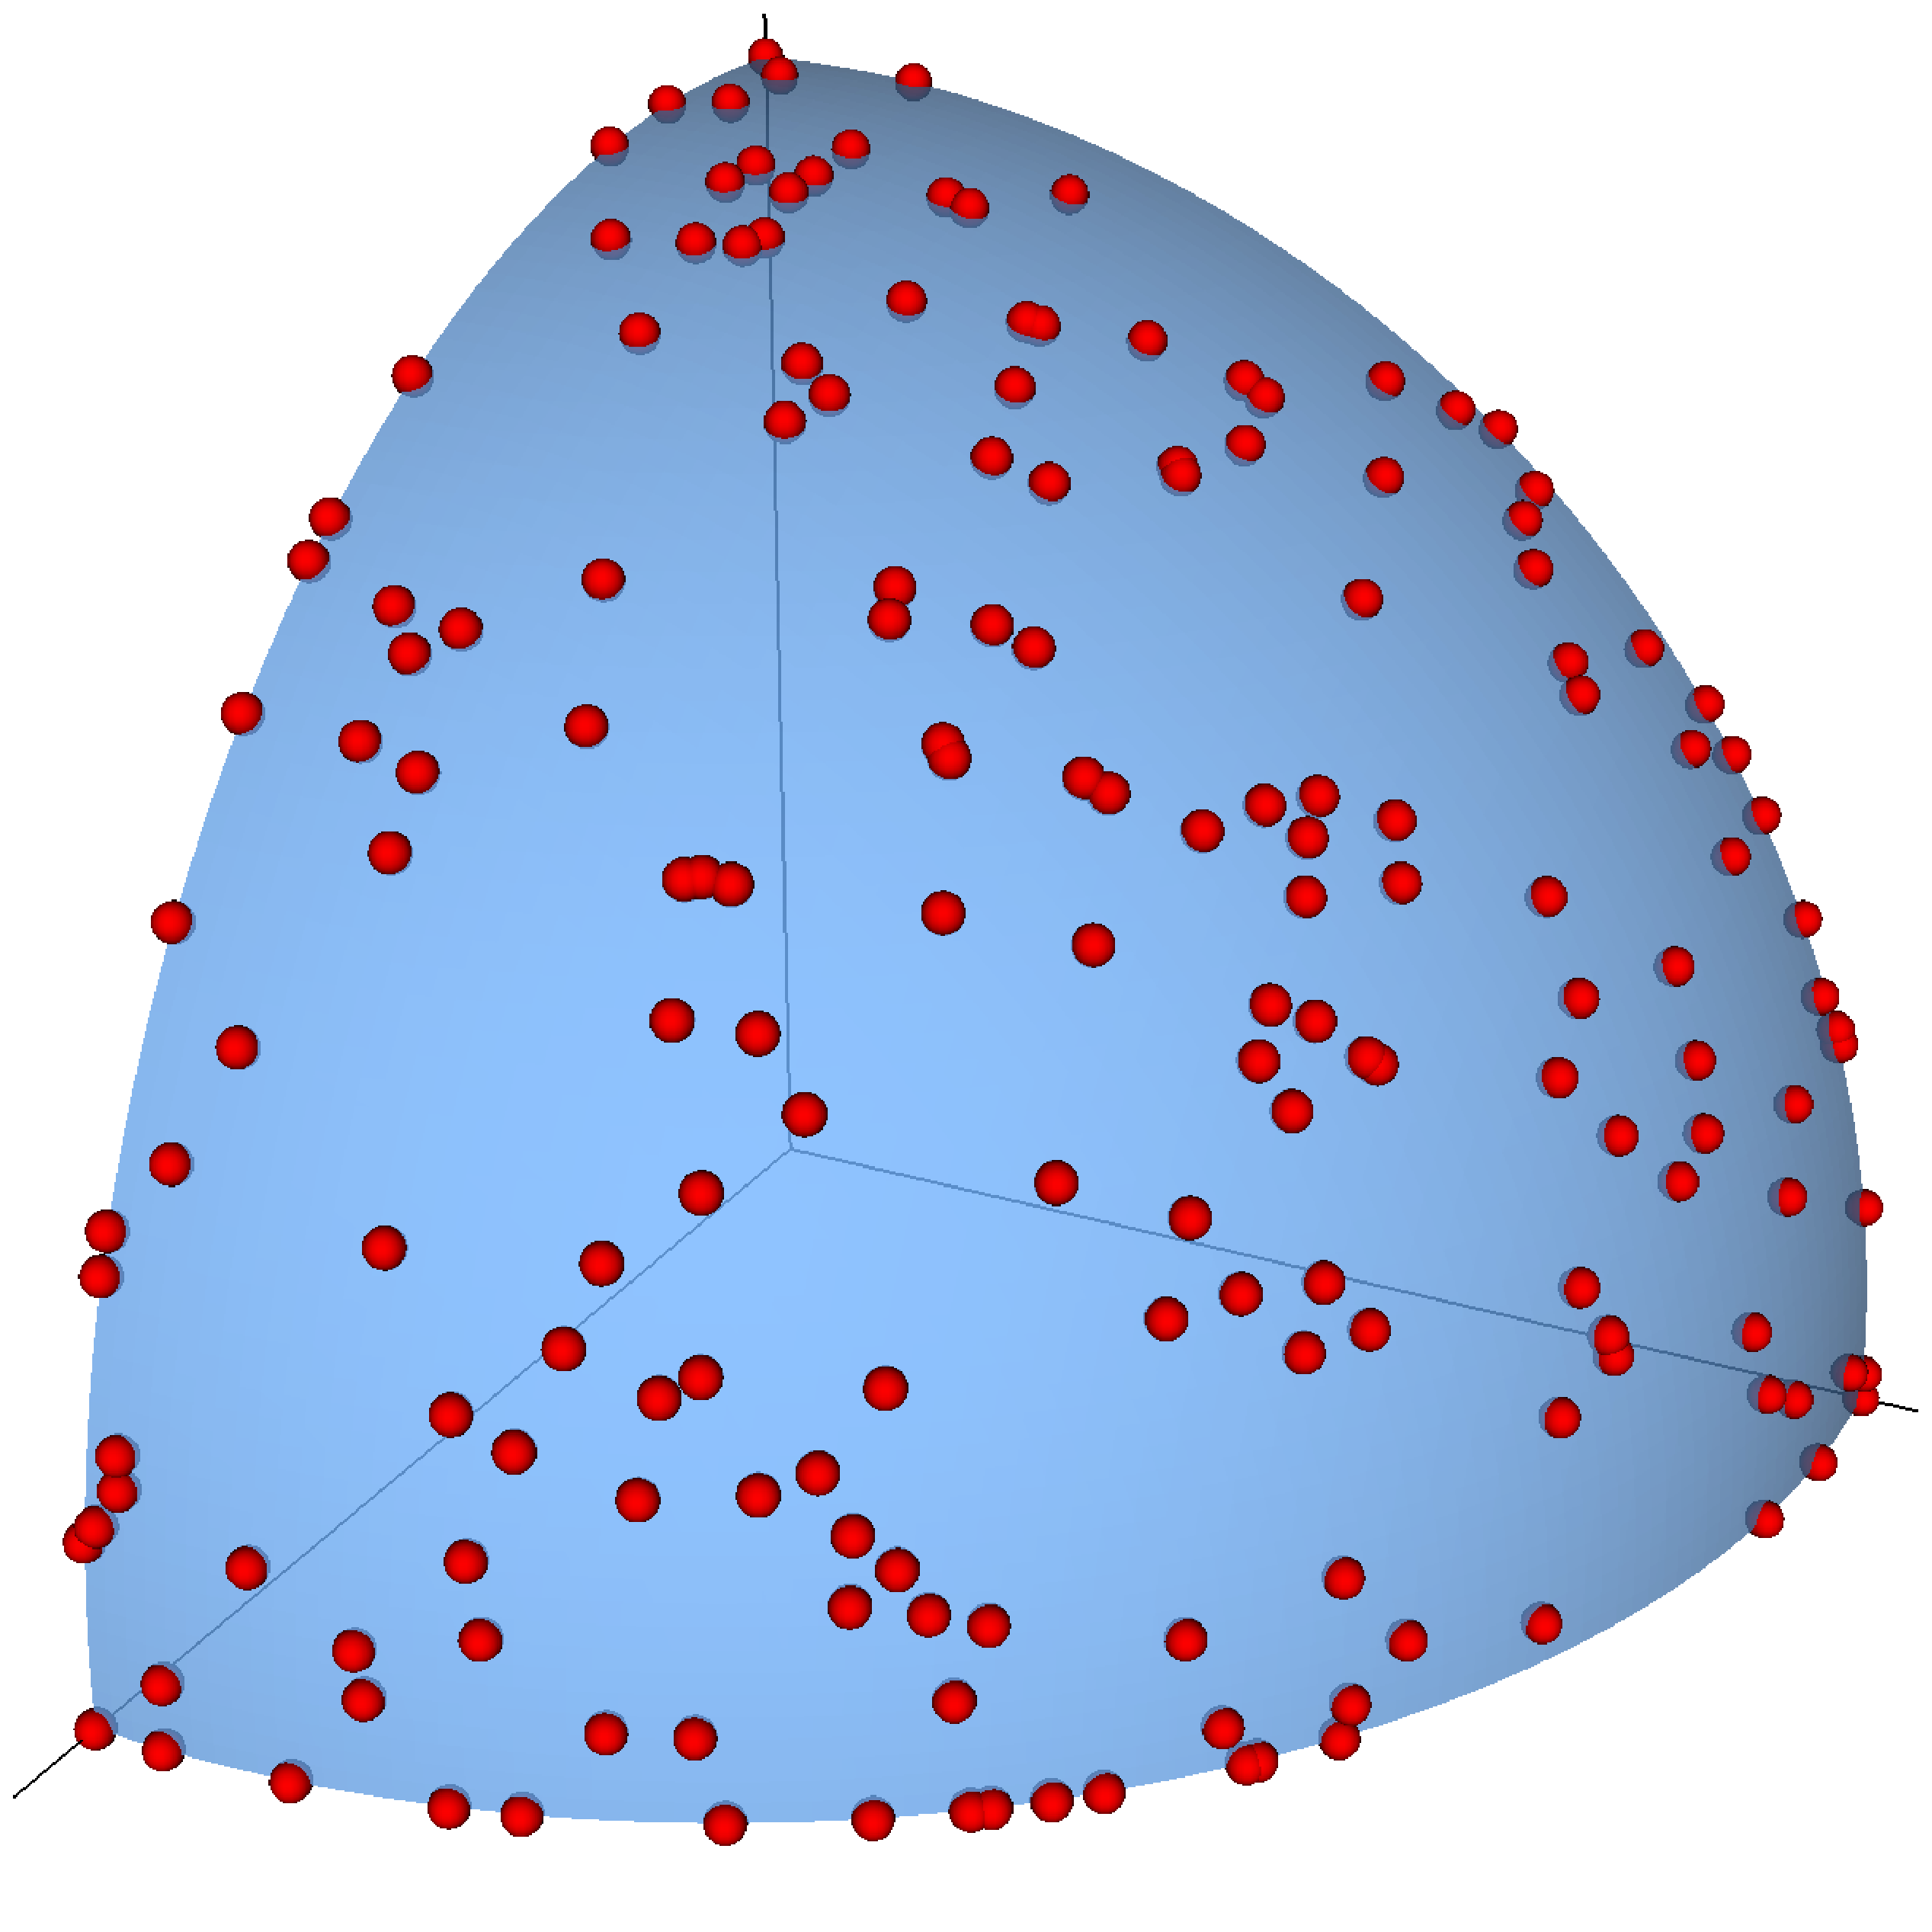
\includegraphics[width=0.36\linewidth]{./figs/res/vtk_DTLZ2_A.eps}}
\subcaptionbox{DTLZ2  (view 2)\label{fig:DTLZ2_B} }[0.49\linewidth]{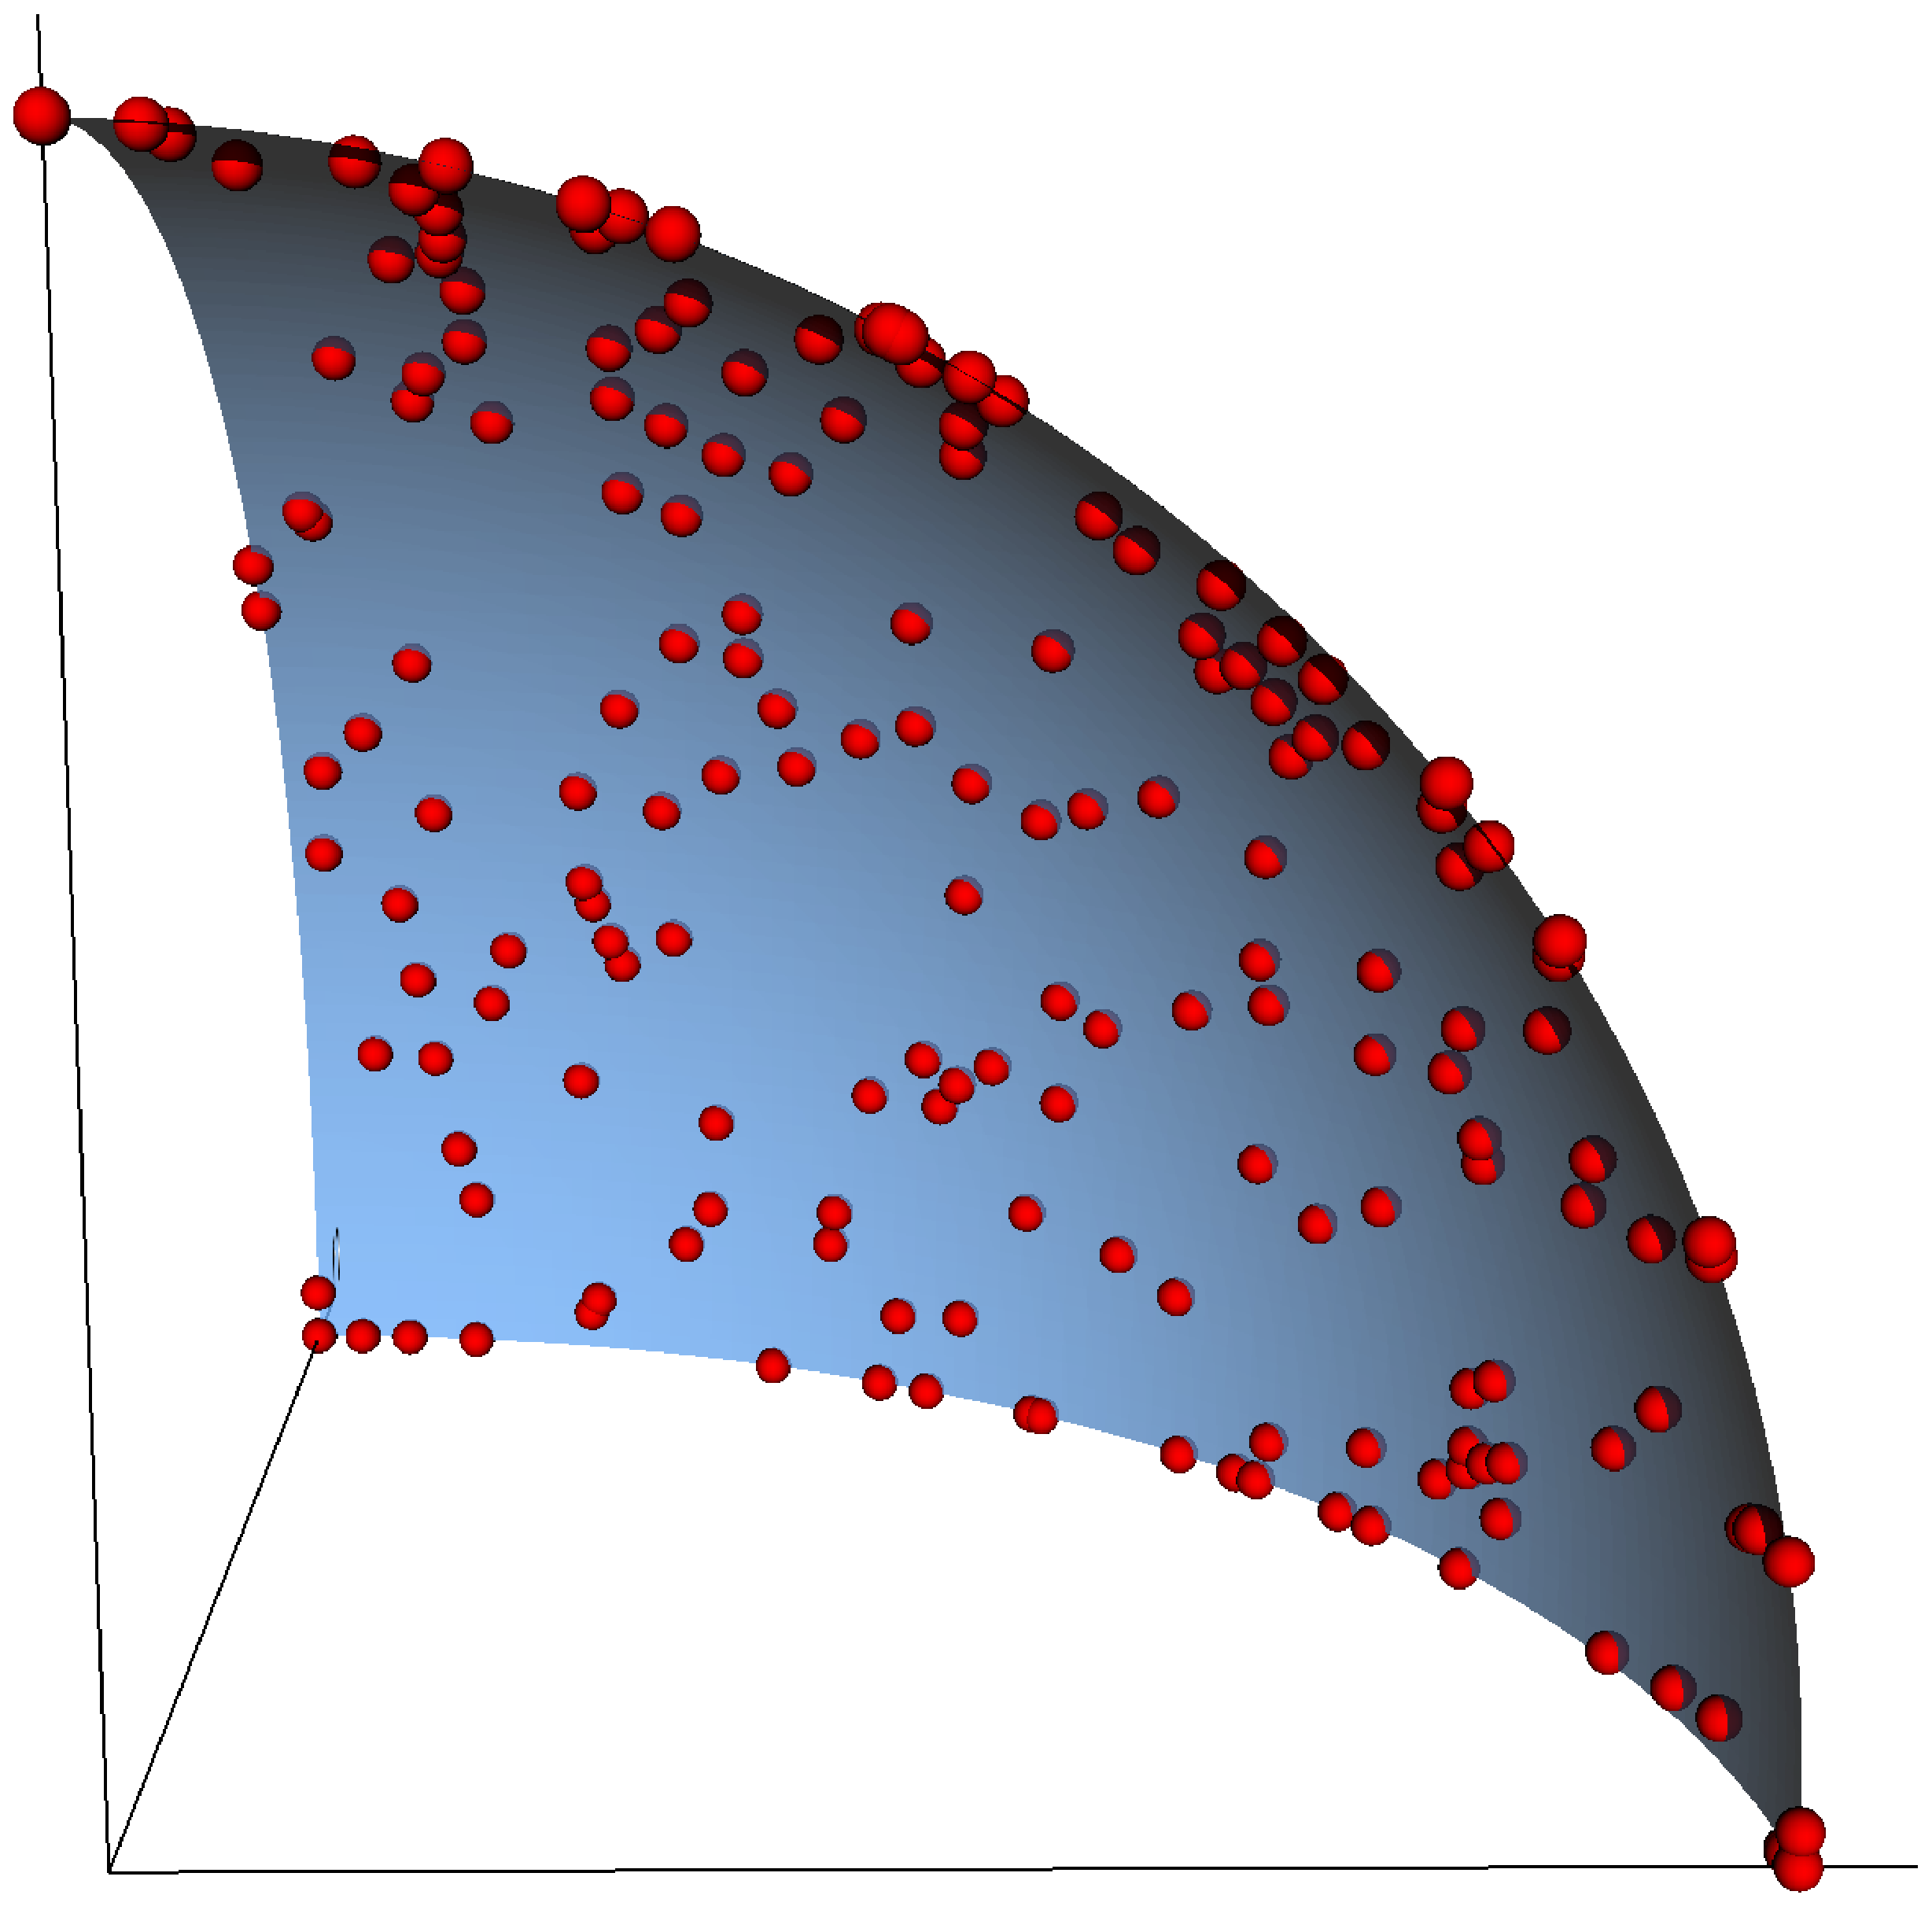
\includegraphics[width=0.36\linewidth]{./figs/res/vtk_DTLZ2_B.eps}}
\subcaptionbox{DTLZ2x (view 1)\label{fig:DTLZ2x_A}}[0.49\linewidth]{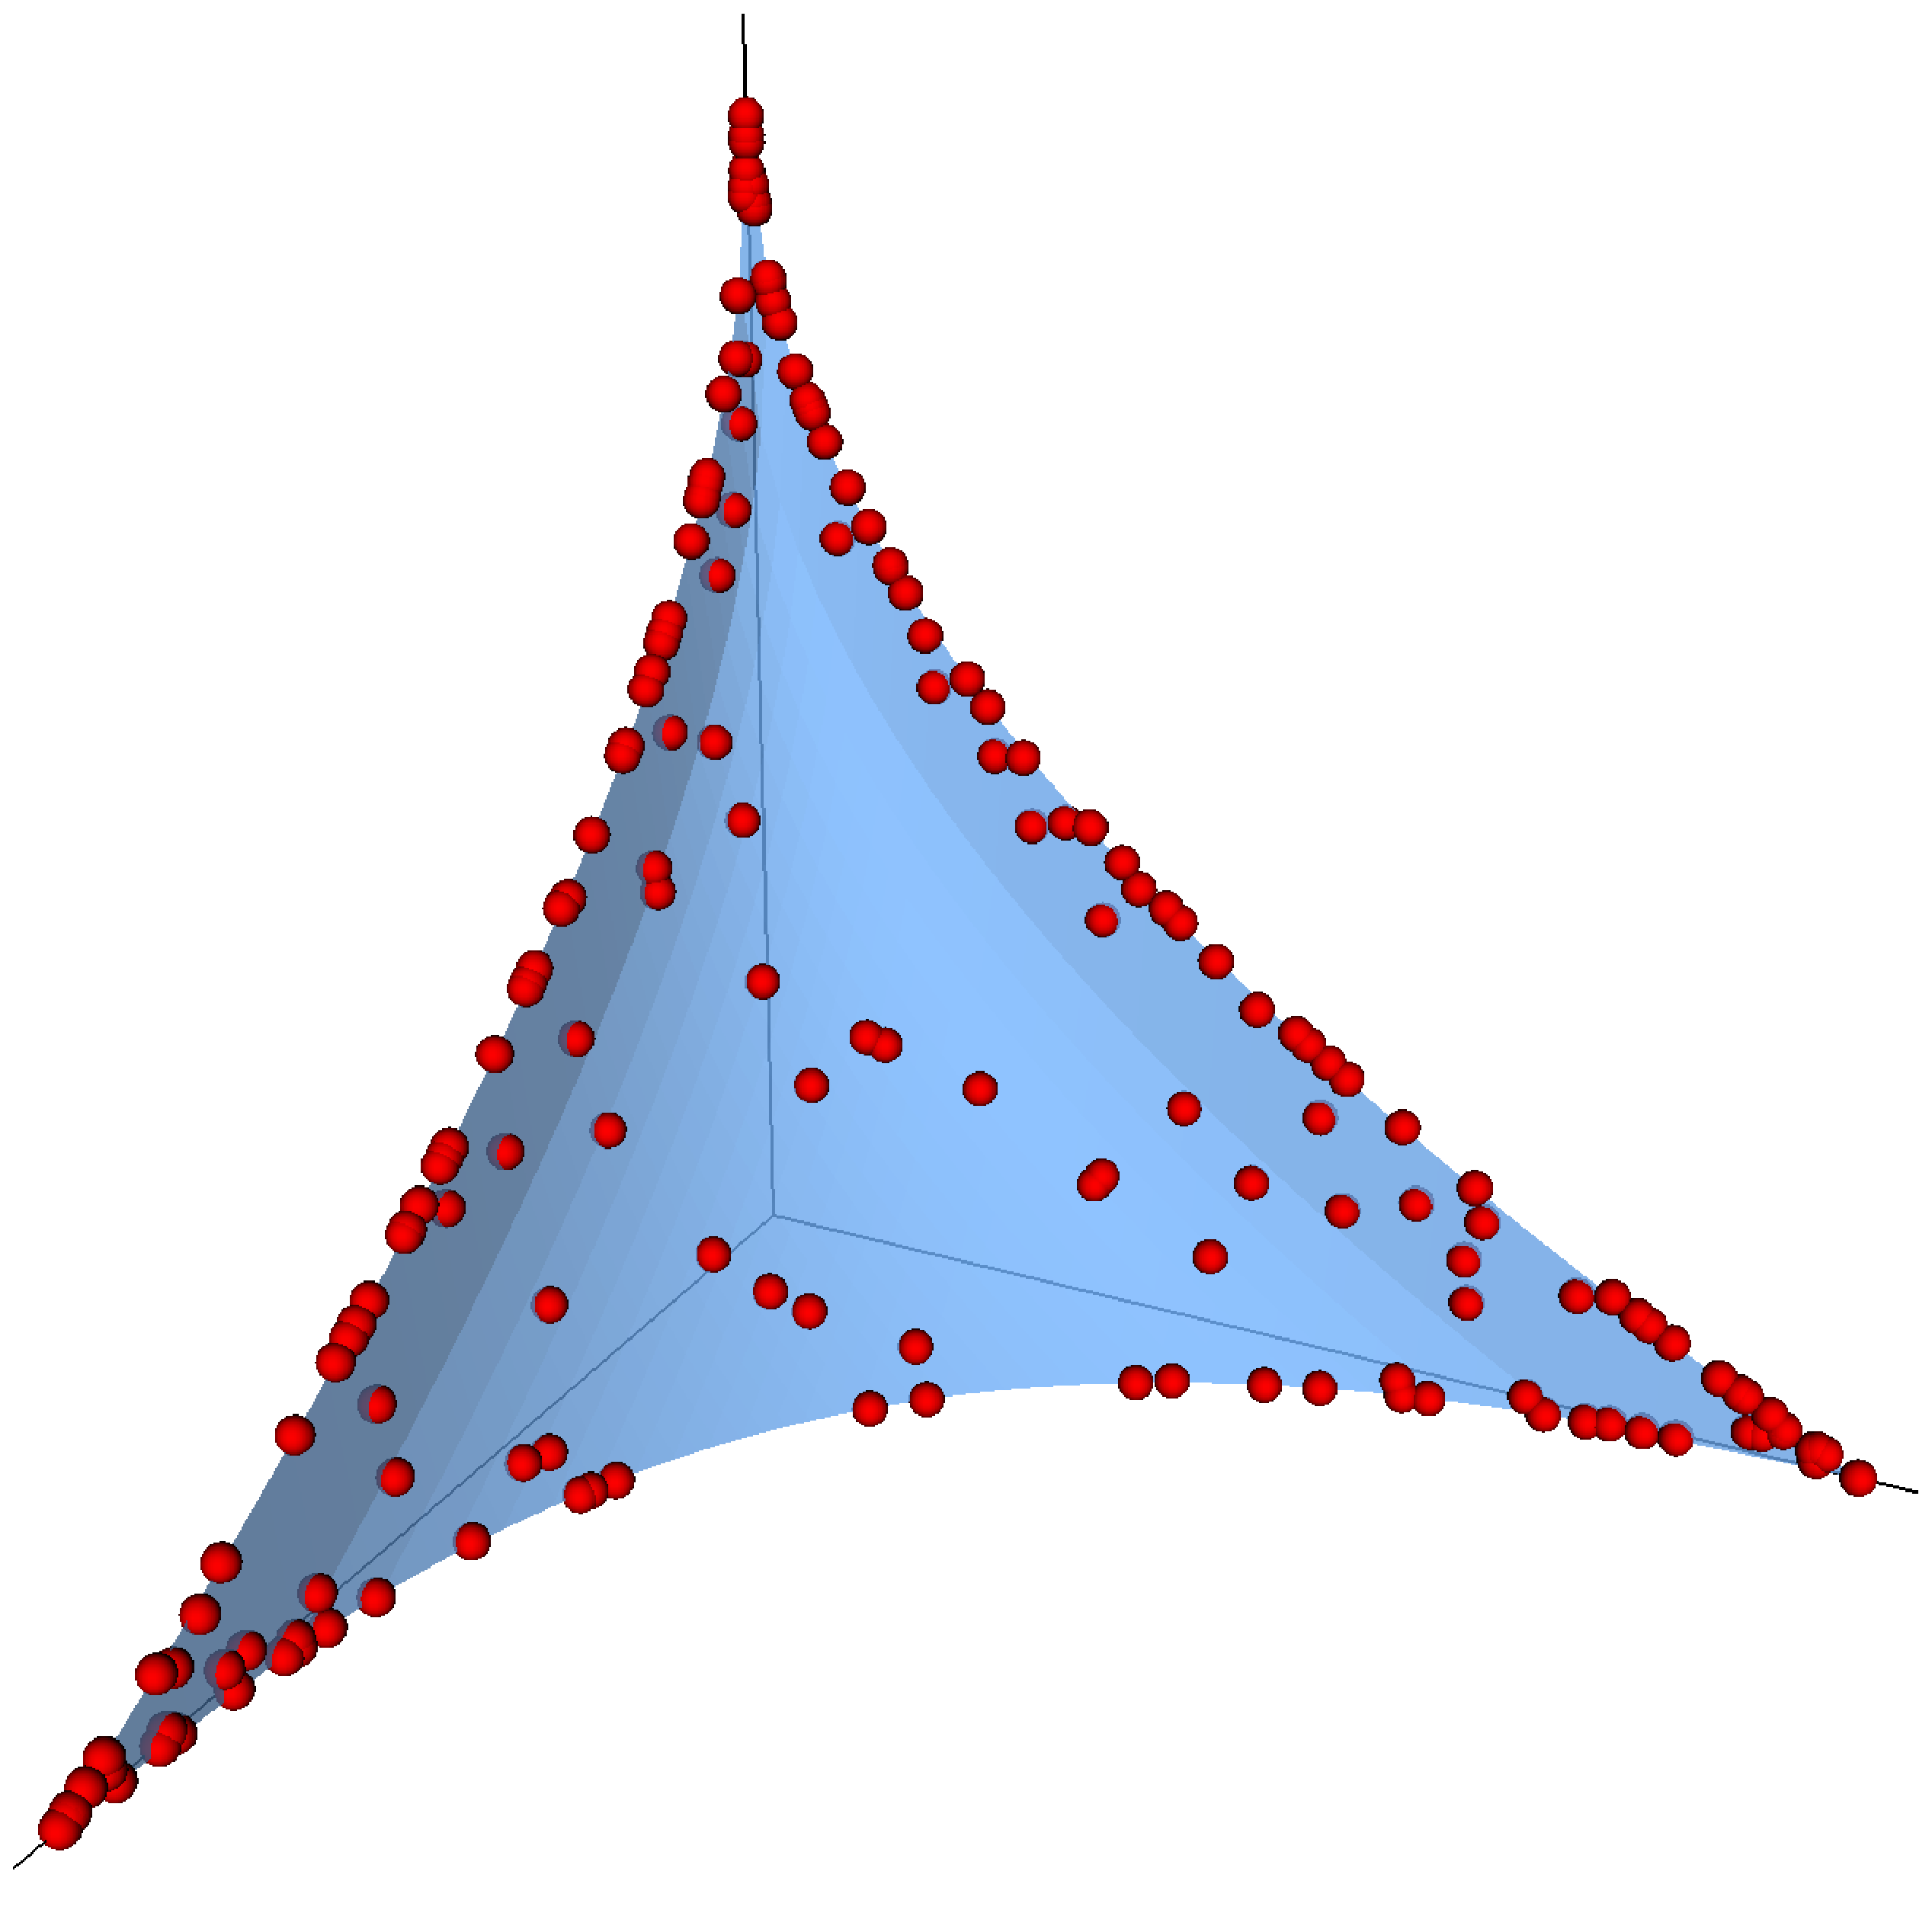
\includegraphics[width=0.38\linewidth]{./figs/res/vtk_DTLZ2x_A.eps}}
\subcaptionbox{DTLZ2x (view 2)\label{fig:DTLZ2x_B}}[0.49\linewidth]{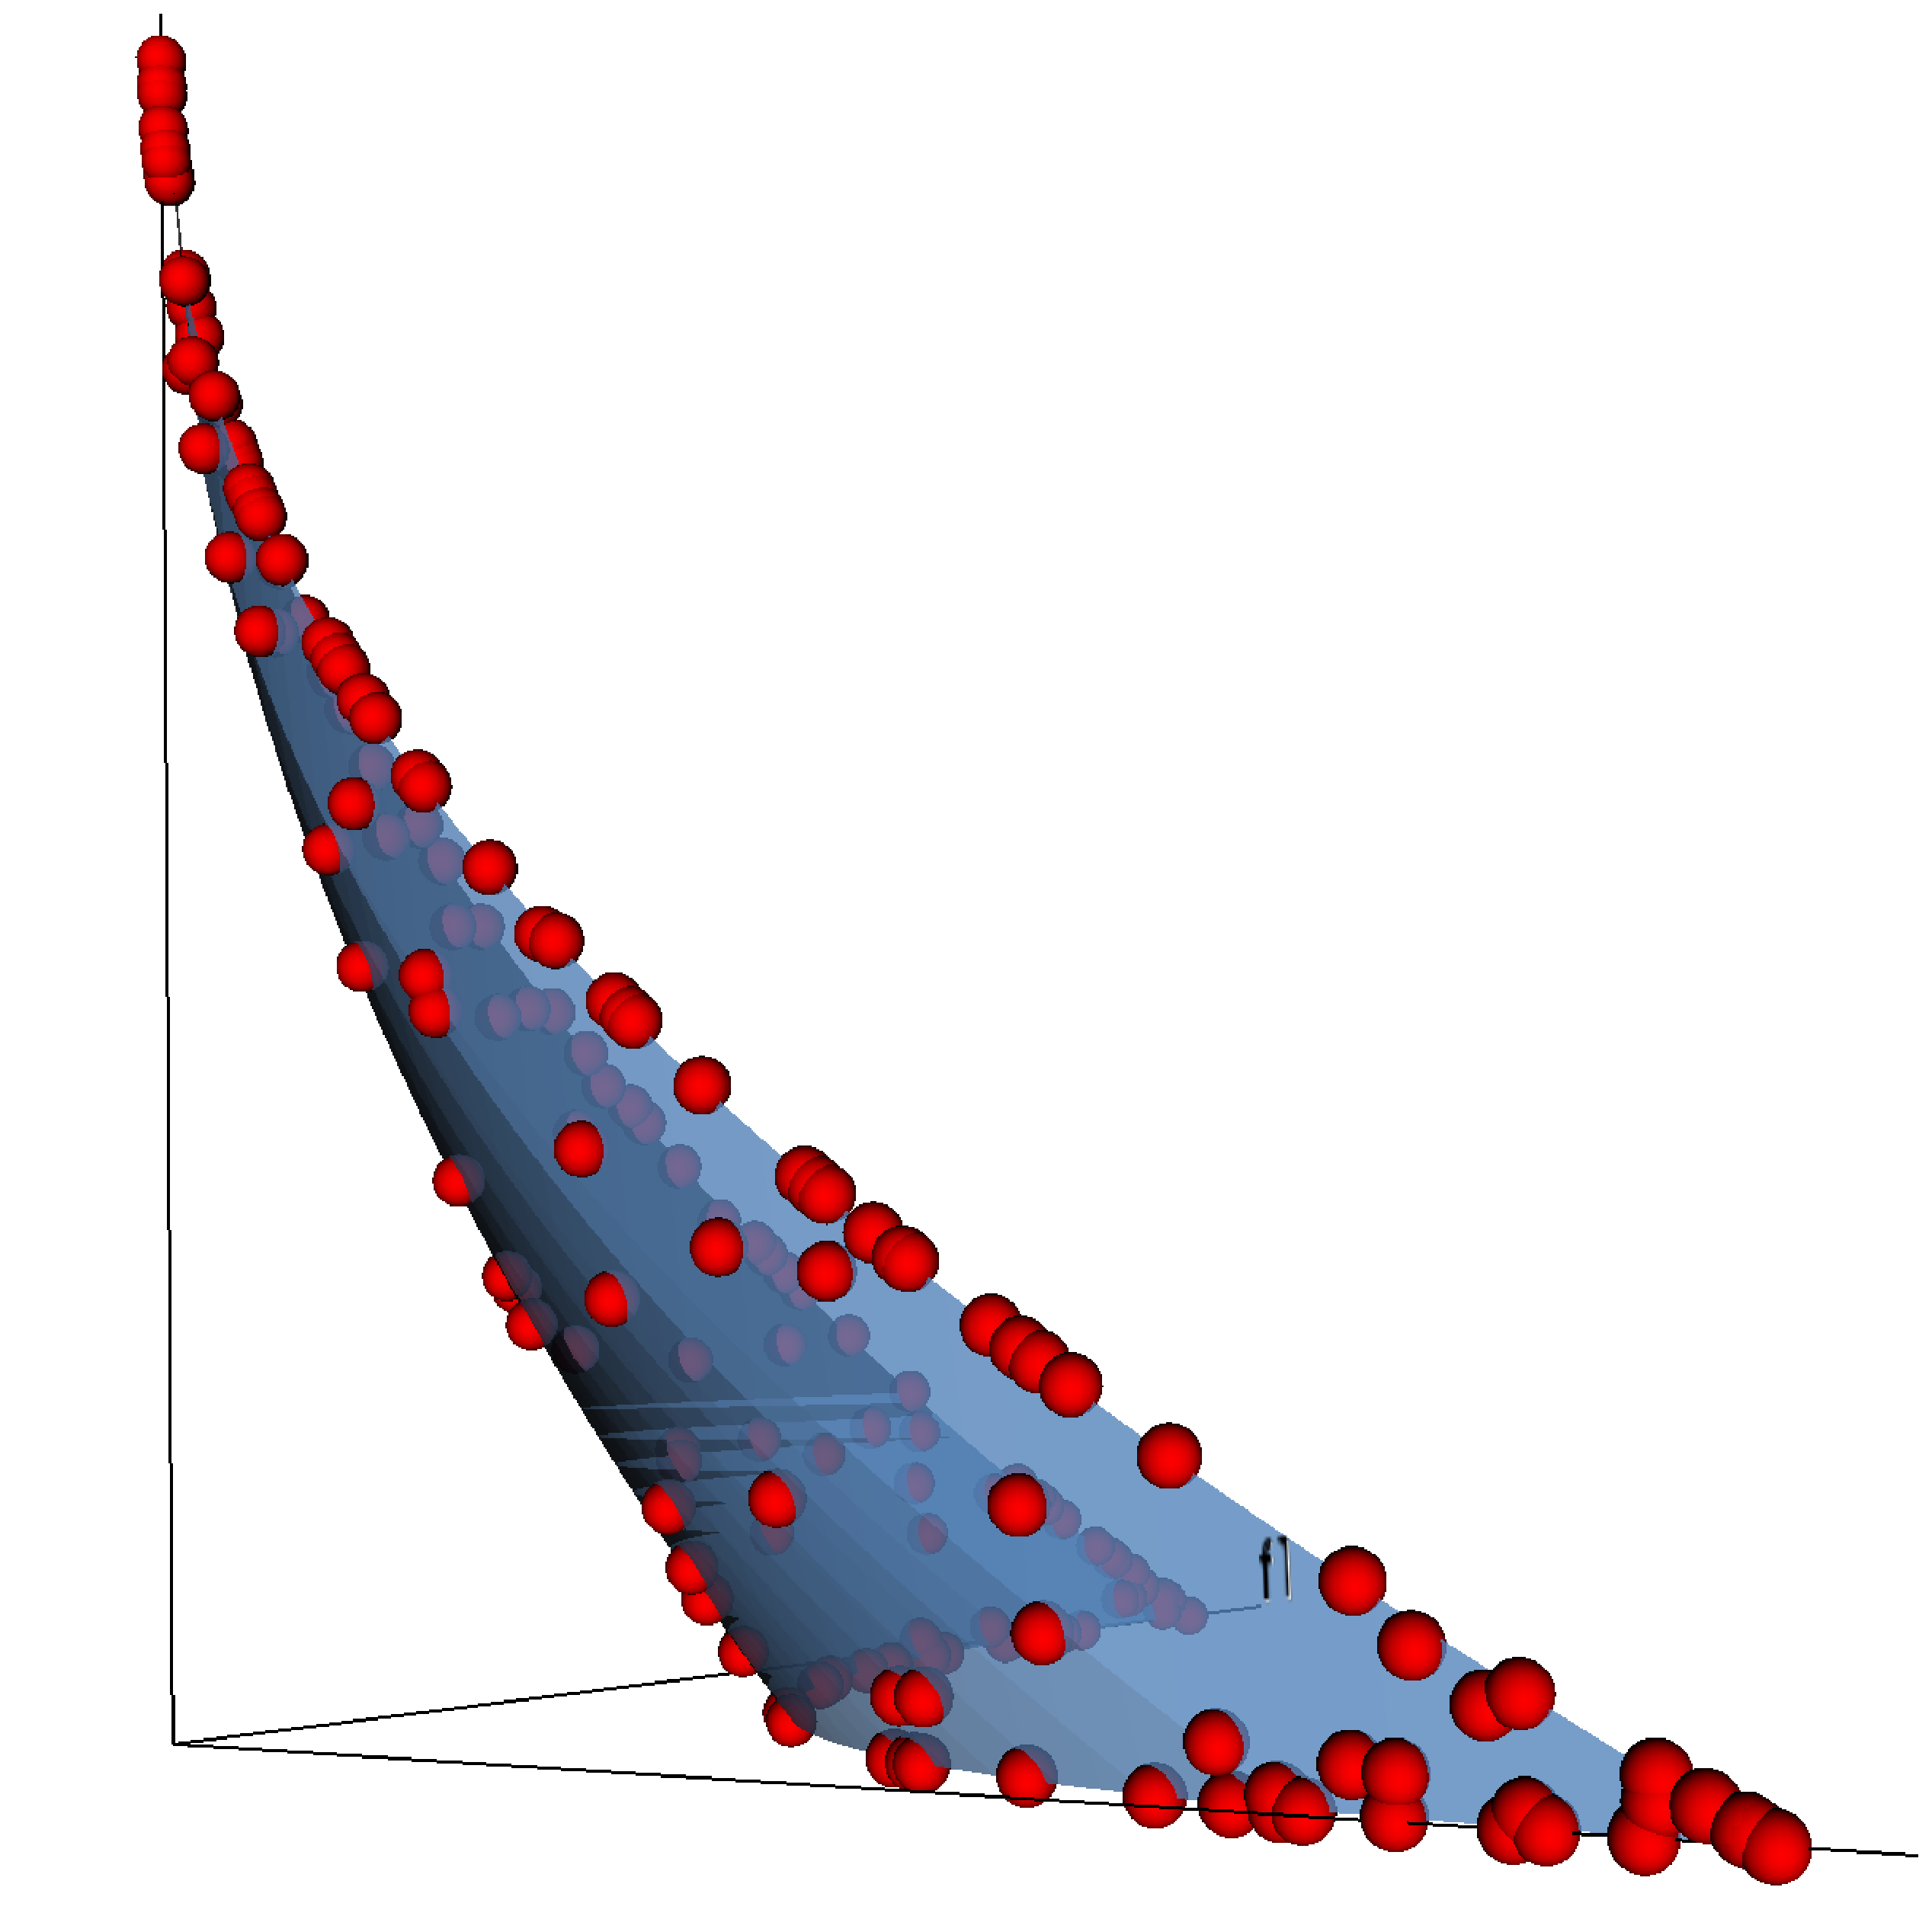
\includegraphics[width=0.36\linewidth]{./figs/res/vtk_DTLZ2x_B.eps}}
\caption{Three-objective problems.}% (a) DTLZ1 (view 1). (b) DTLZ1 (view 2). (c) DTLZ2 (view 1). (d)
%DTLZ2 (view 2). (e) DTLZ2x (view 1). (f) DTLZ2x (view 2).}
\label{fig:three-objA}
\end{figure*}

\begin{figure*} \centering
\subcaptionbox{DTLZ2c (view 1)\label{fig:DTLZ2c_A}}[0.49\linewidth]{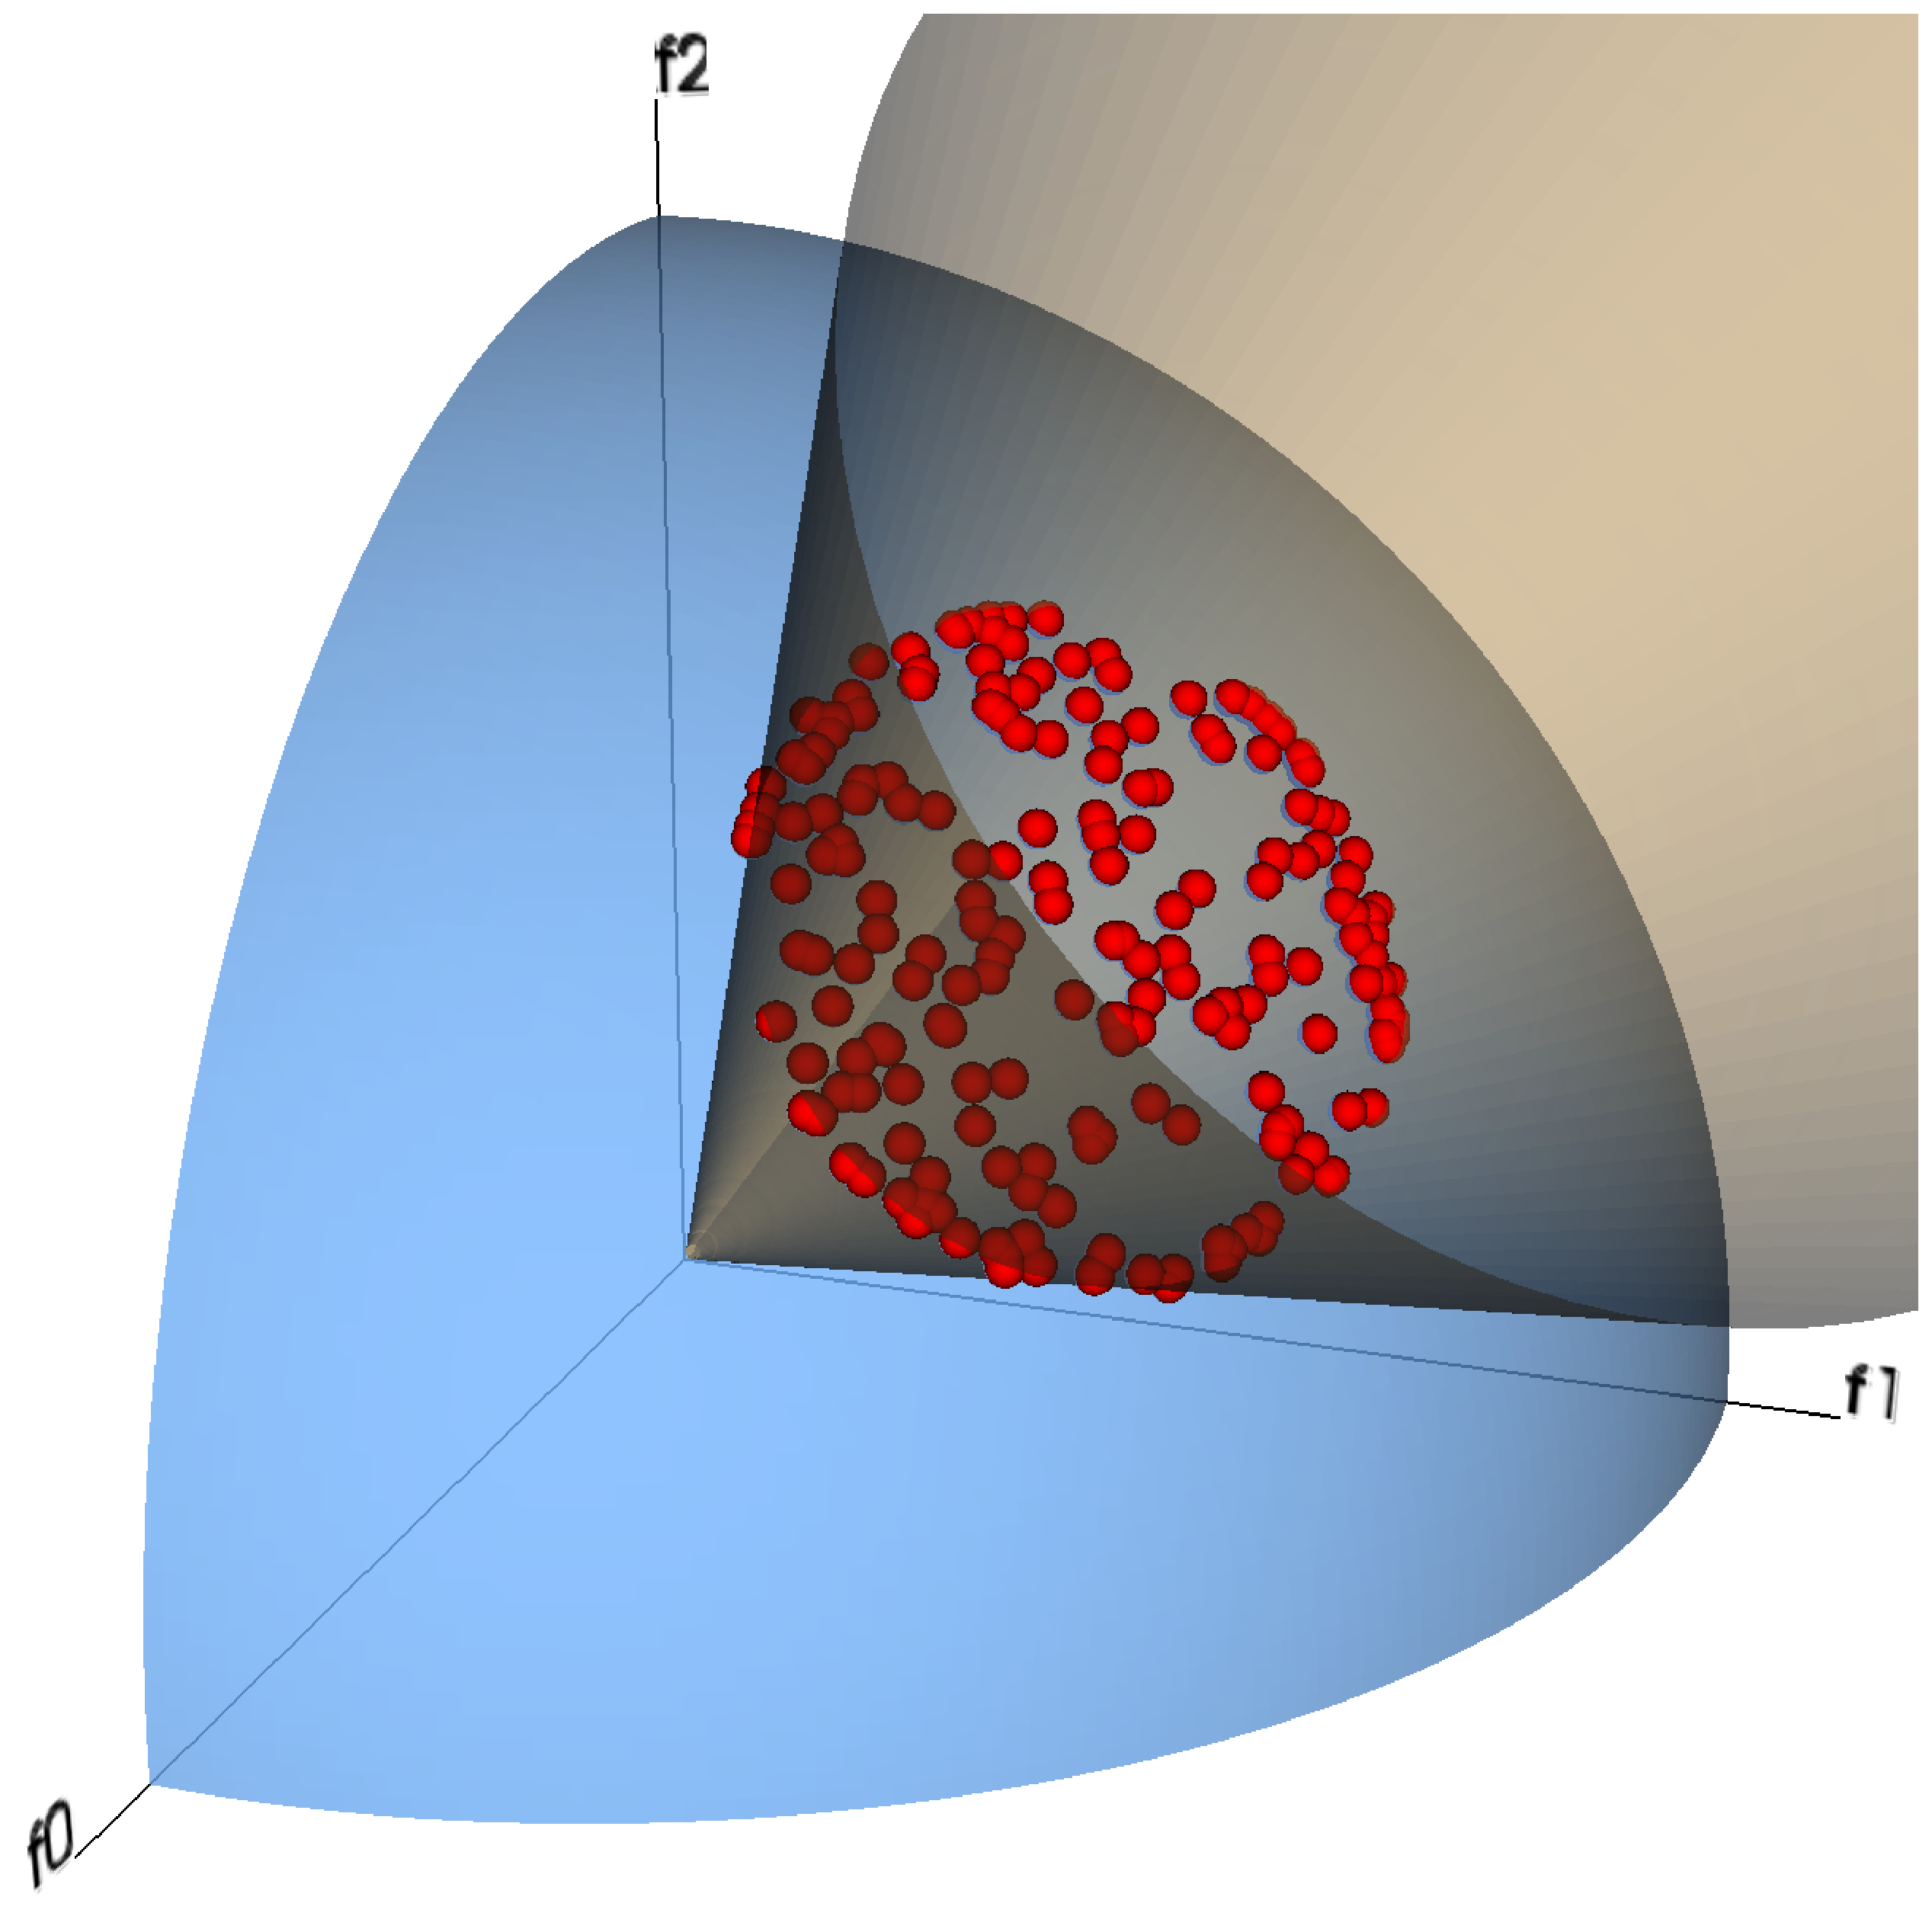
\includegraphics[width=0.36\linewidth]{./figs/res/vtk_DTLZ2c_A.eps}}
\subcaptionbox{DTLZ2c (view 2)\label{fig:DTLZ2c_B}}[0.49\linewidth]{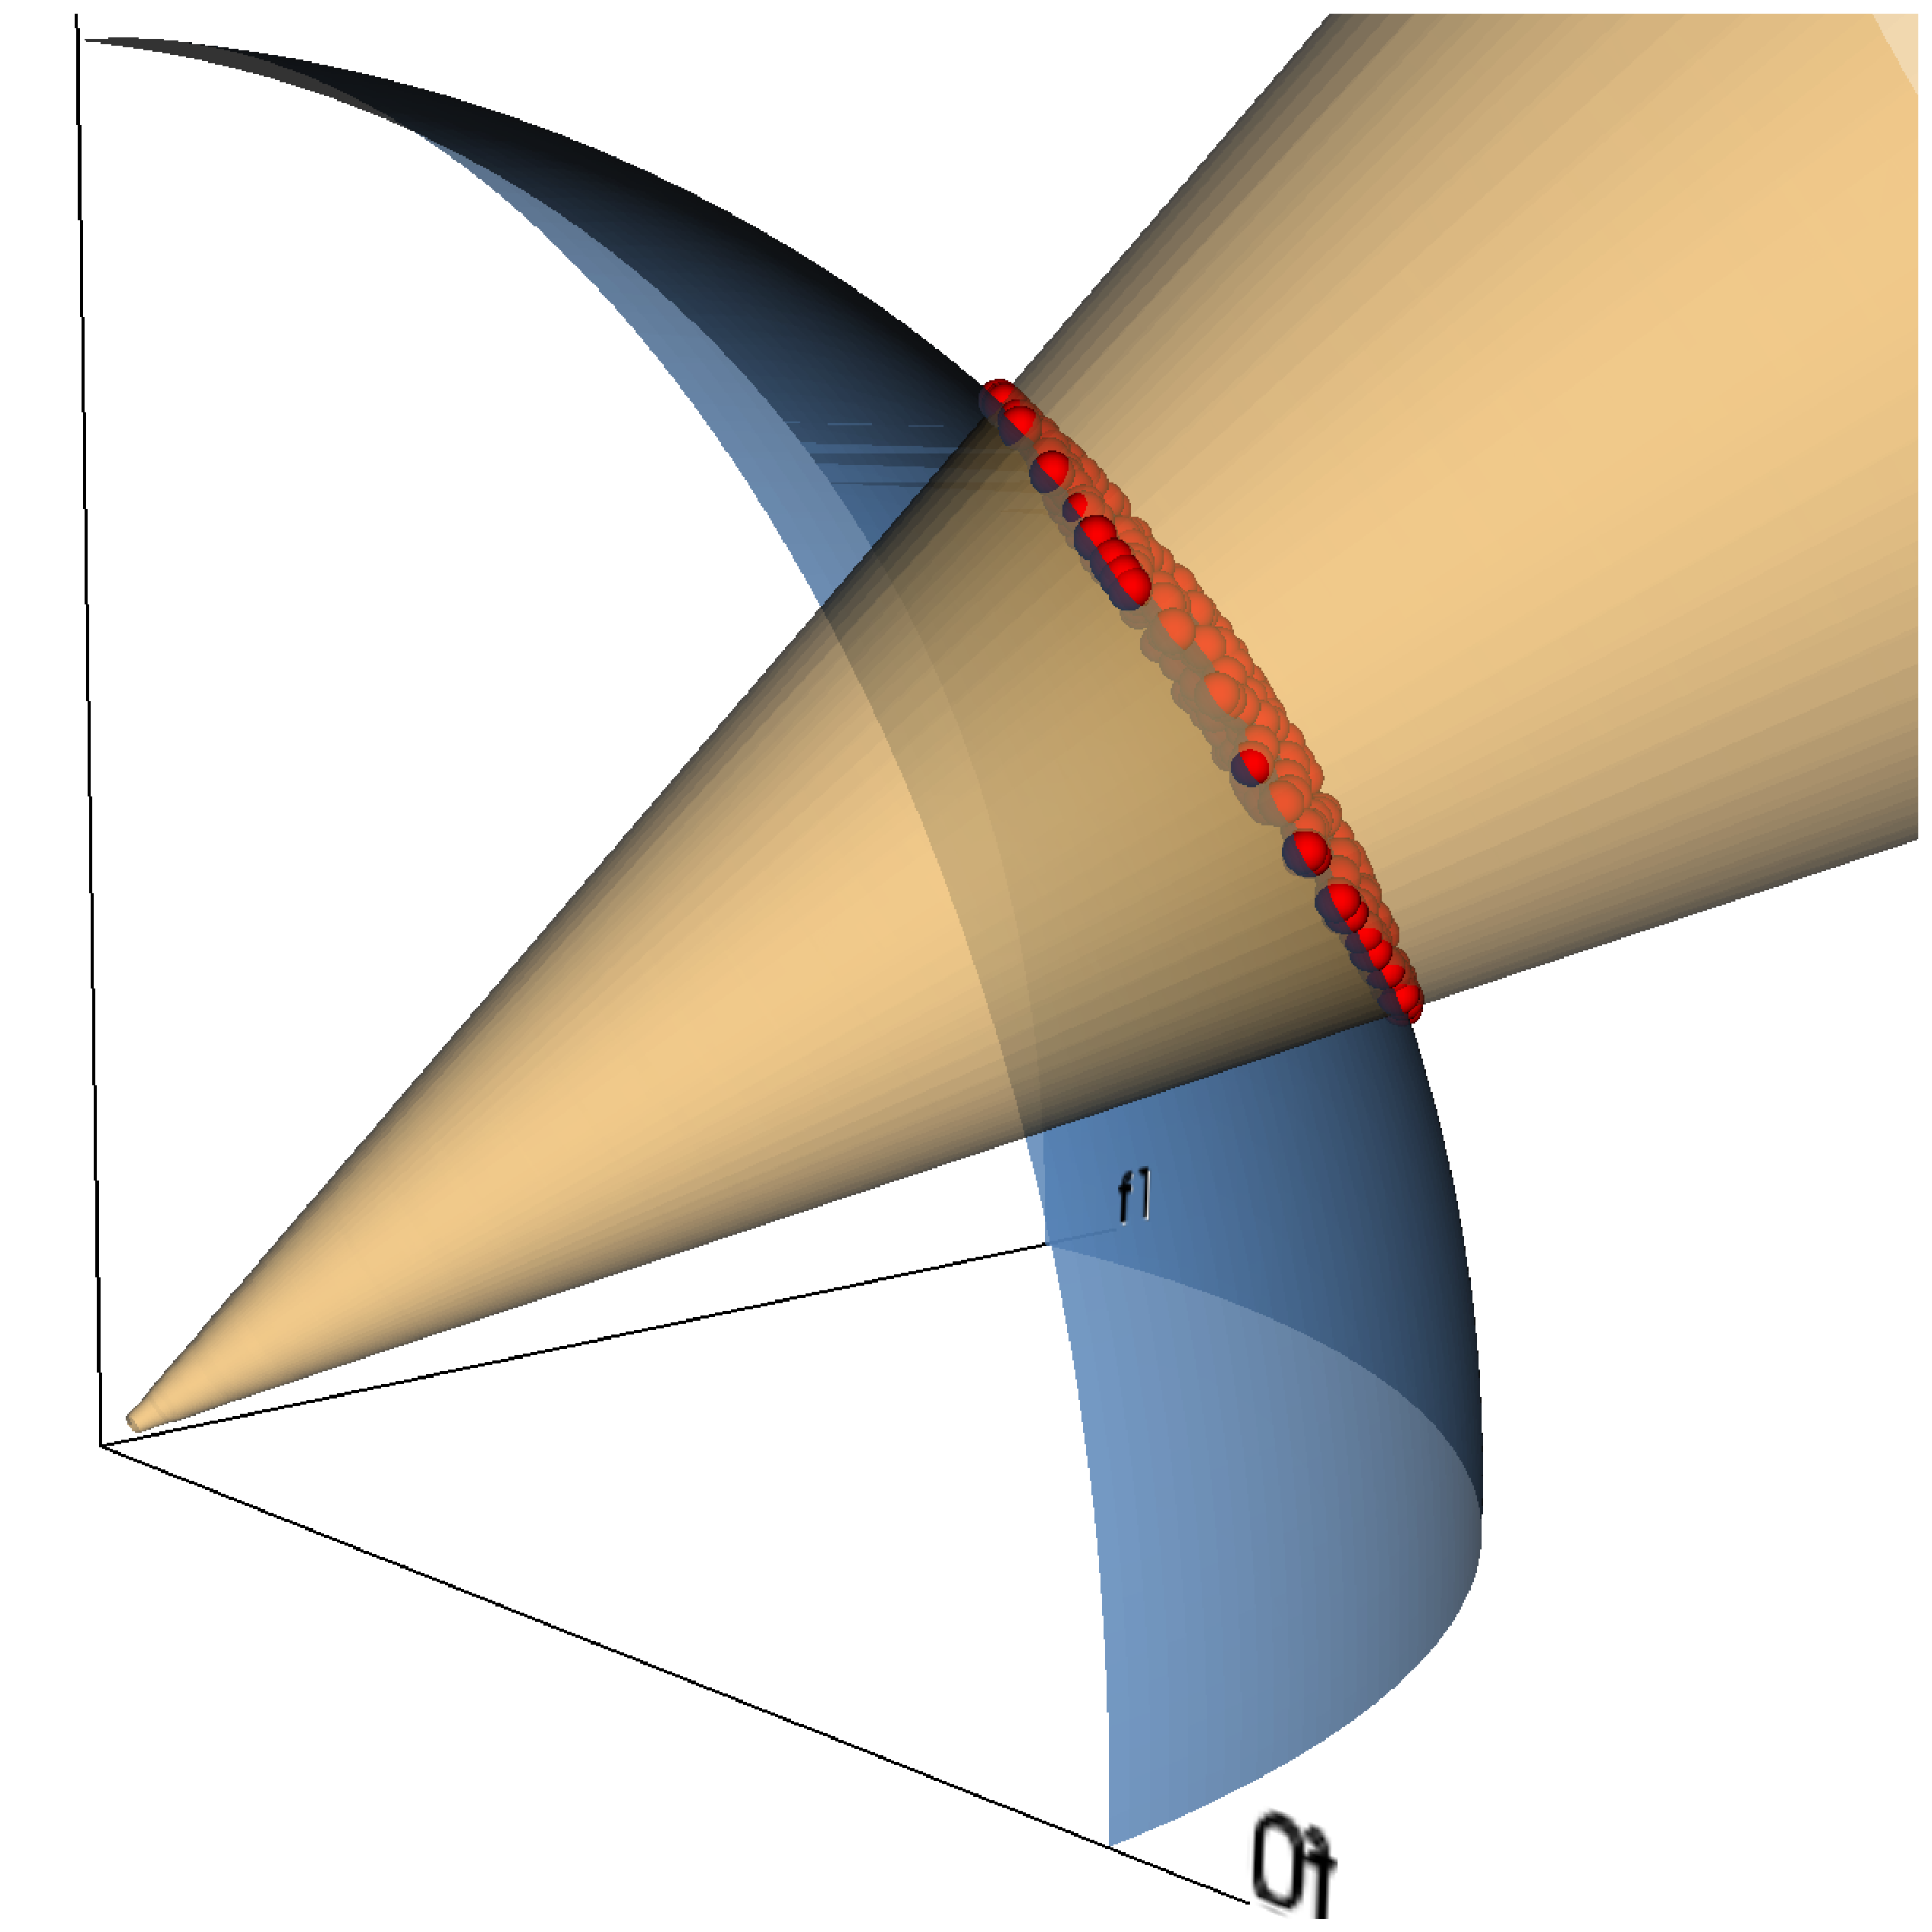
\includegraphics[width=0.36\linewidth]{./figs/res/vtk_DTLZ2c_B.eps}}
\subcaptionbox{SUQ1   (view 1)\label{fig:SUQ1_A}  }[0.49\linewidth]{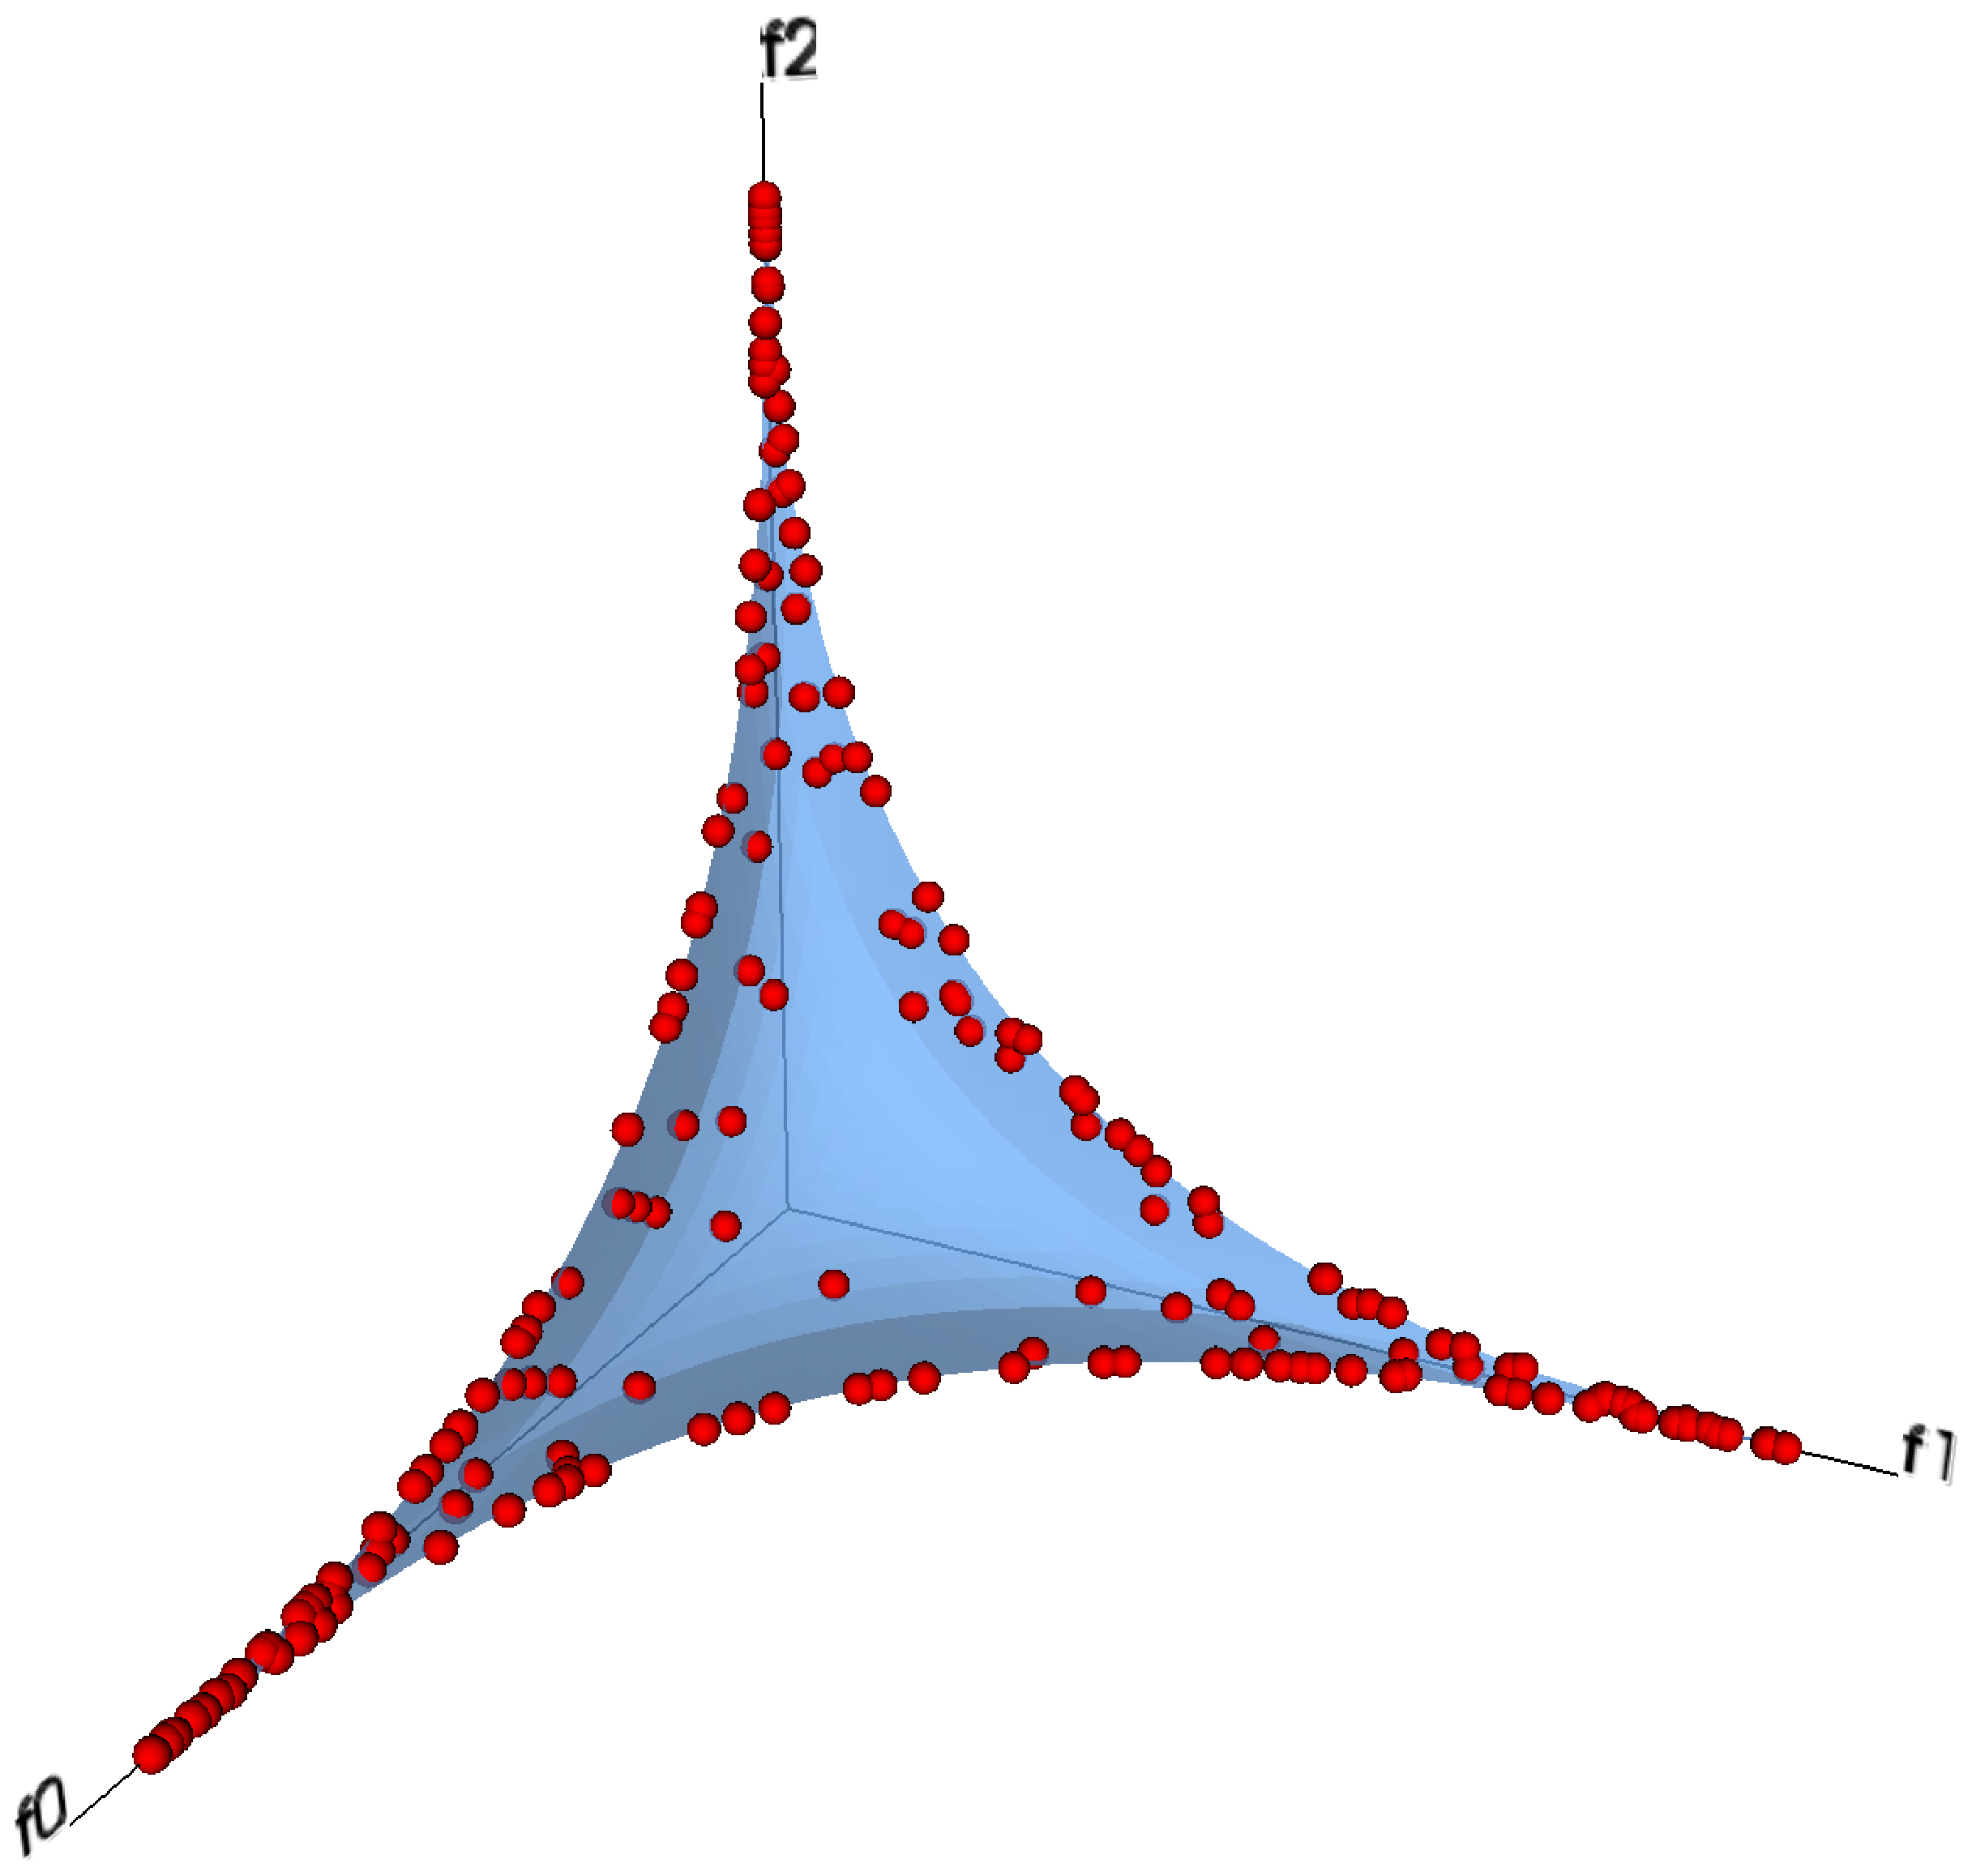
\includegraphics[width=0.36\linewidth]{./figs/res/vtk_SUQ1_A.eps}}
\subcaptionbox{SUQ1   (view 2)\label{fig:SUQ1_B}  }[0.49\linewidth]{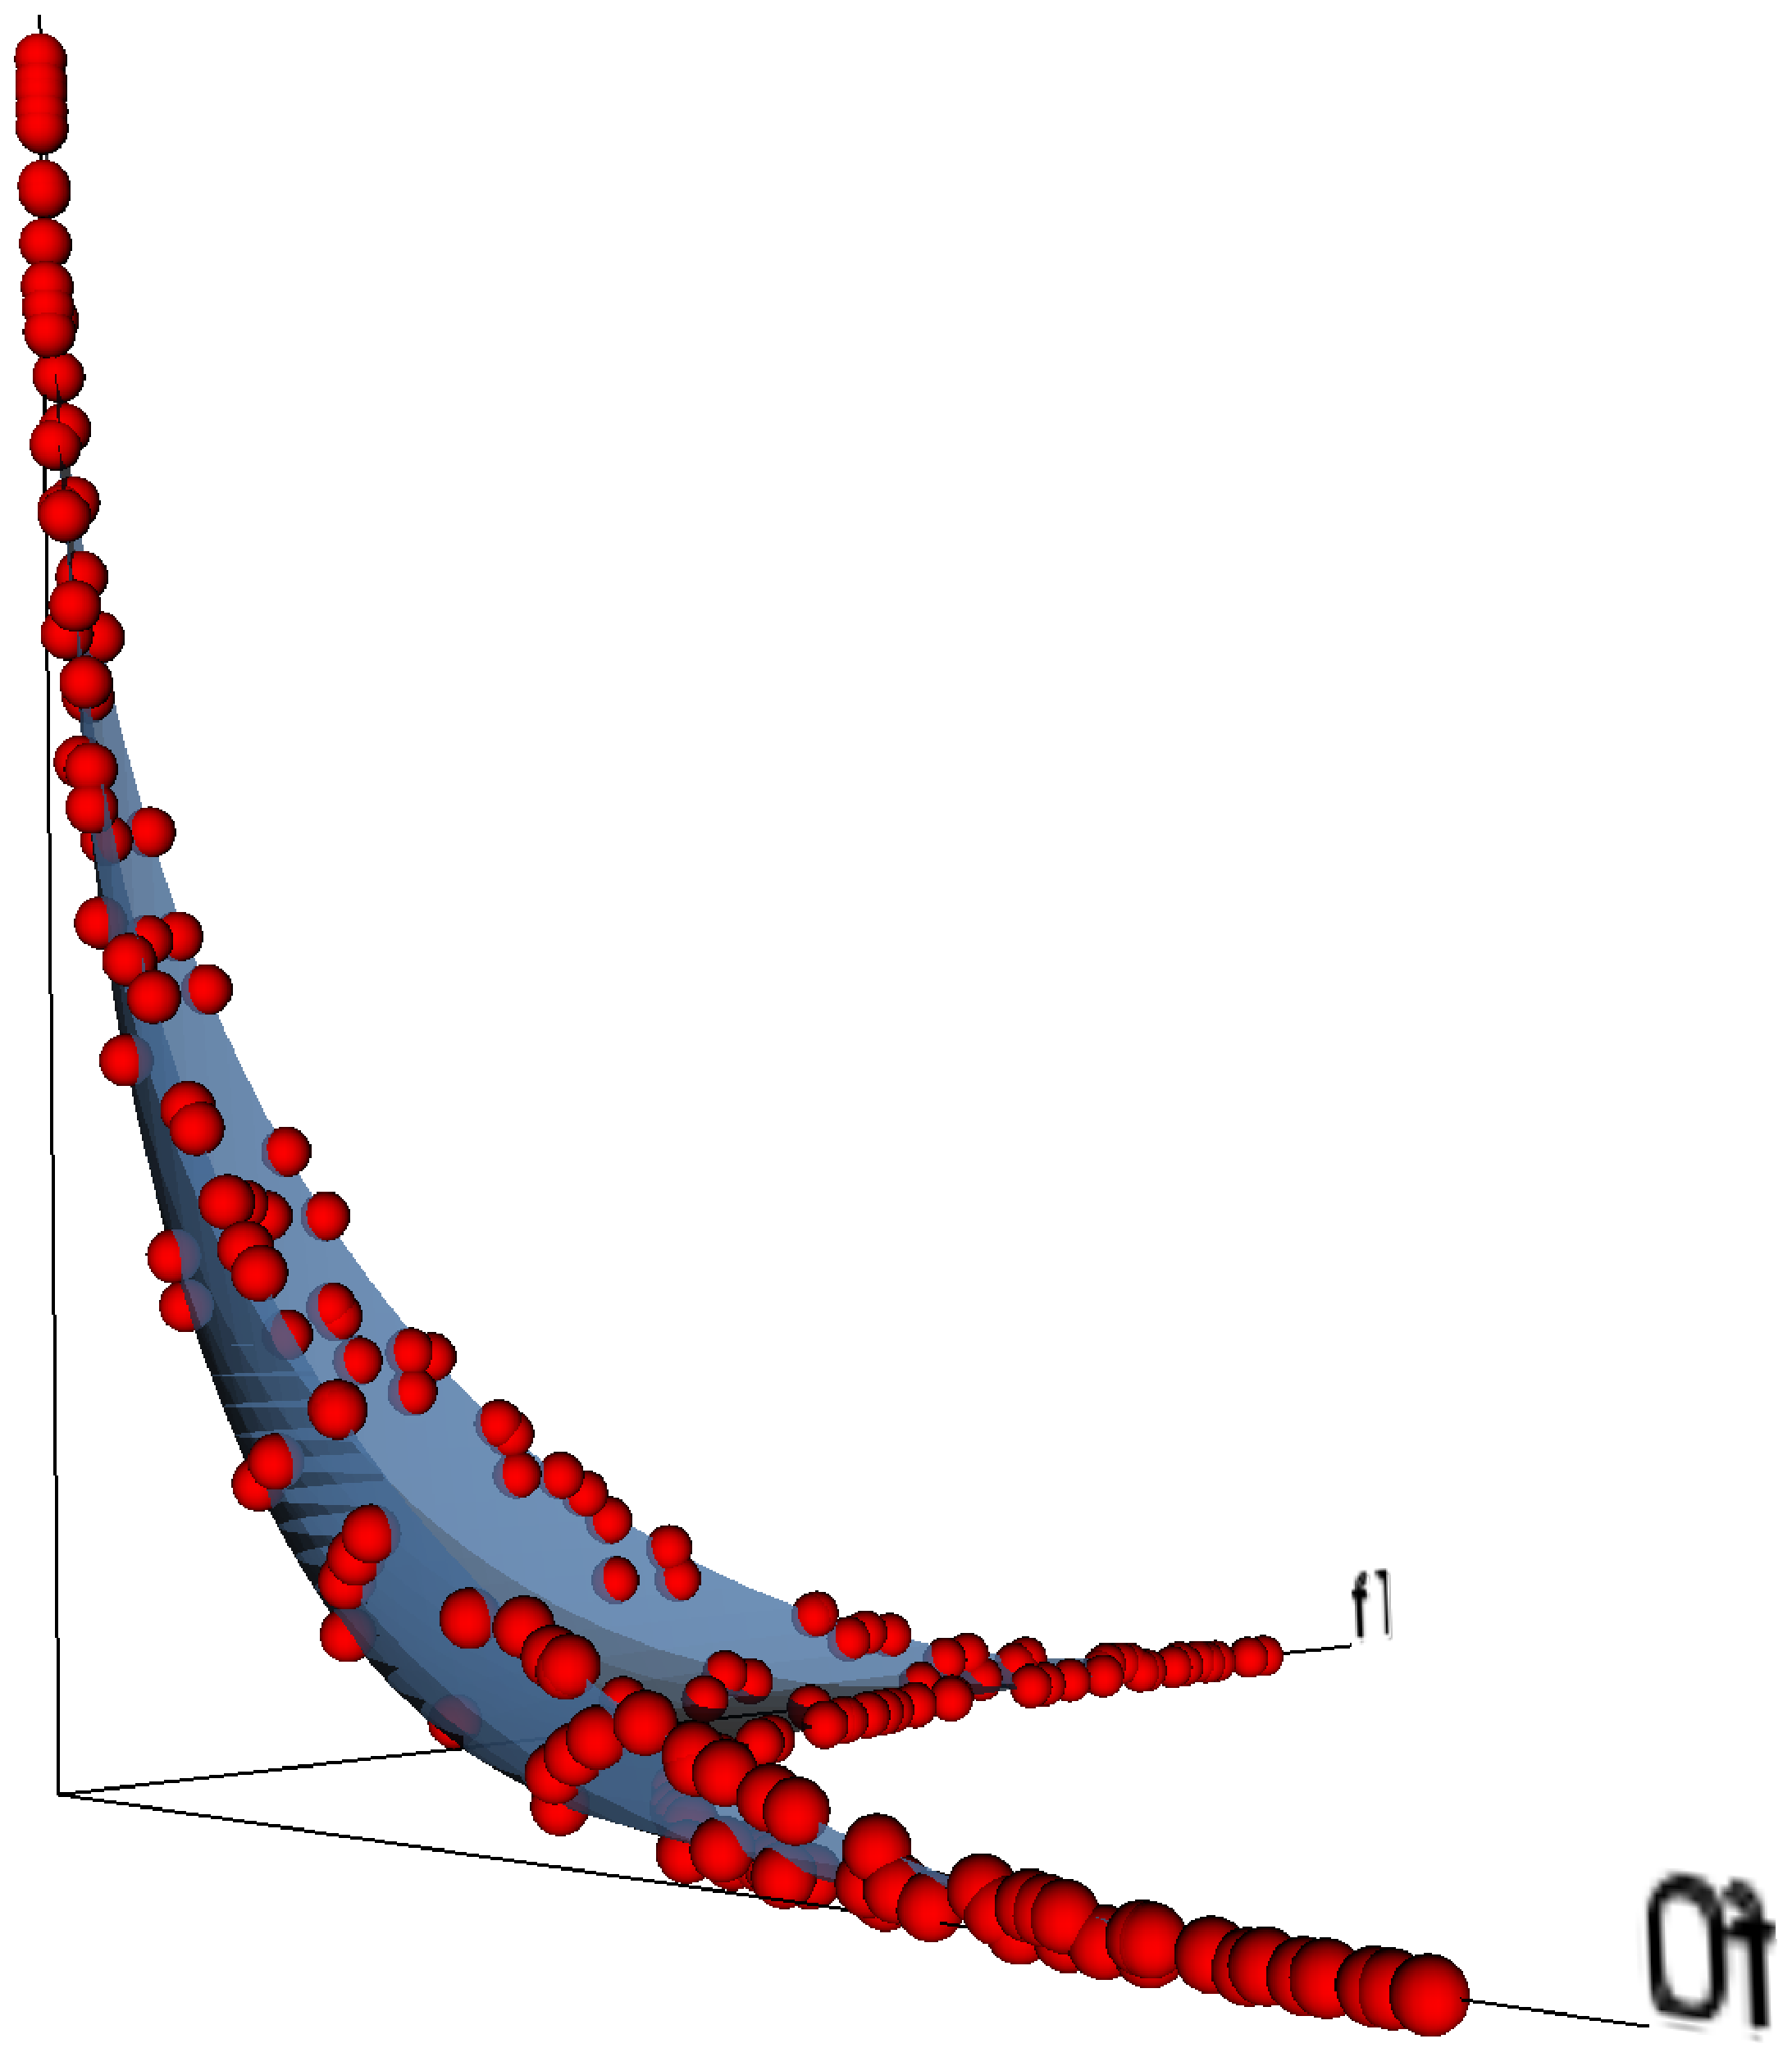
\includegraphics[width=0.31\linewidth]{./figs/res/vtk_SUQ1_B.eps}}
\subcaptionbox{SUQ2   (view 1)\label{fig:SUQ2_A}  }[0.49\linewidth]{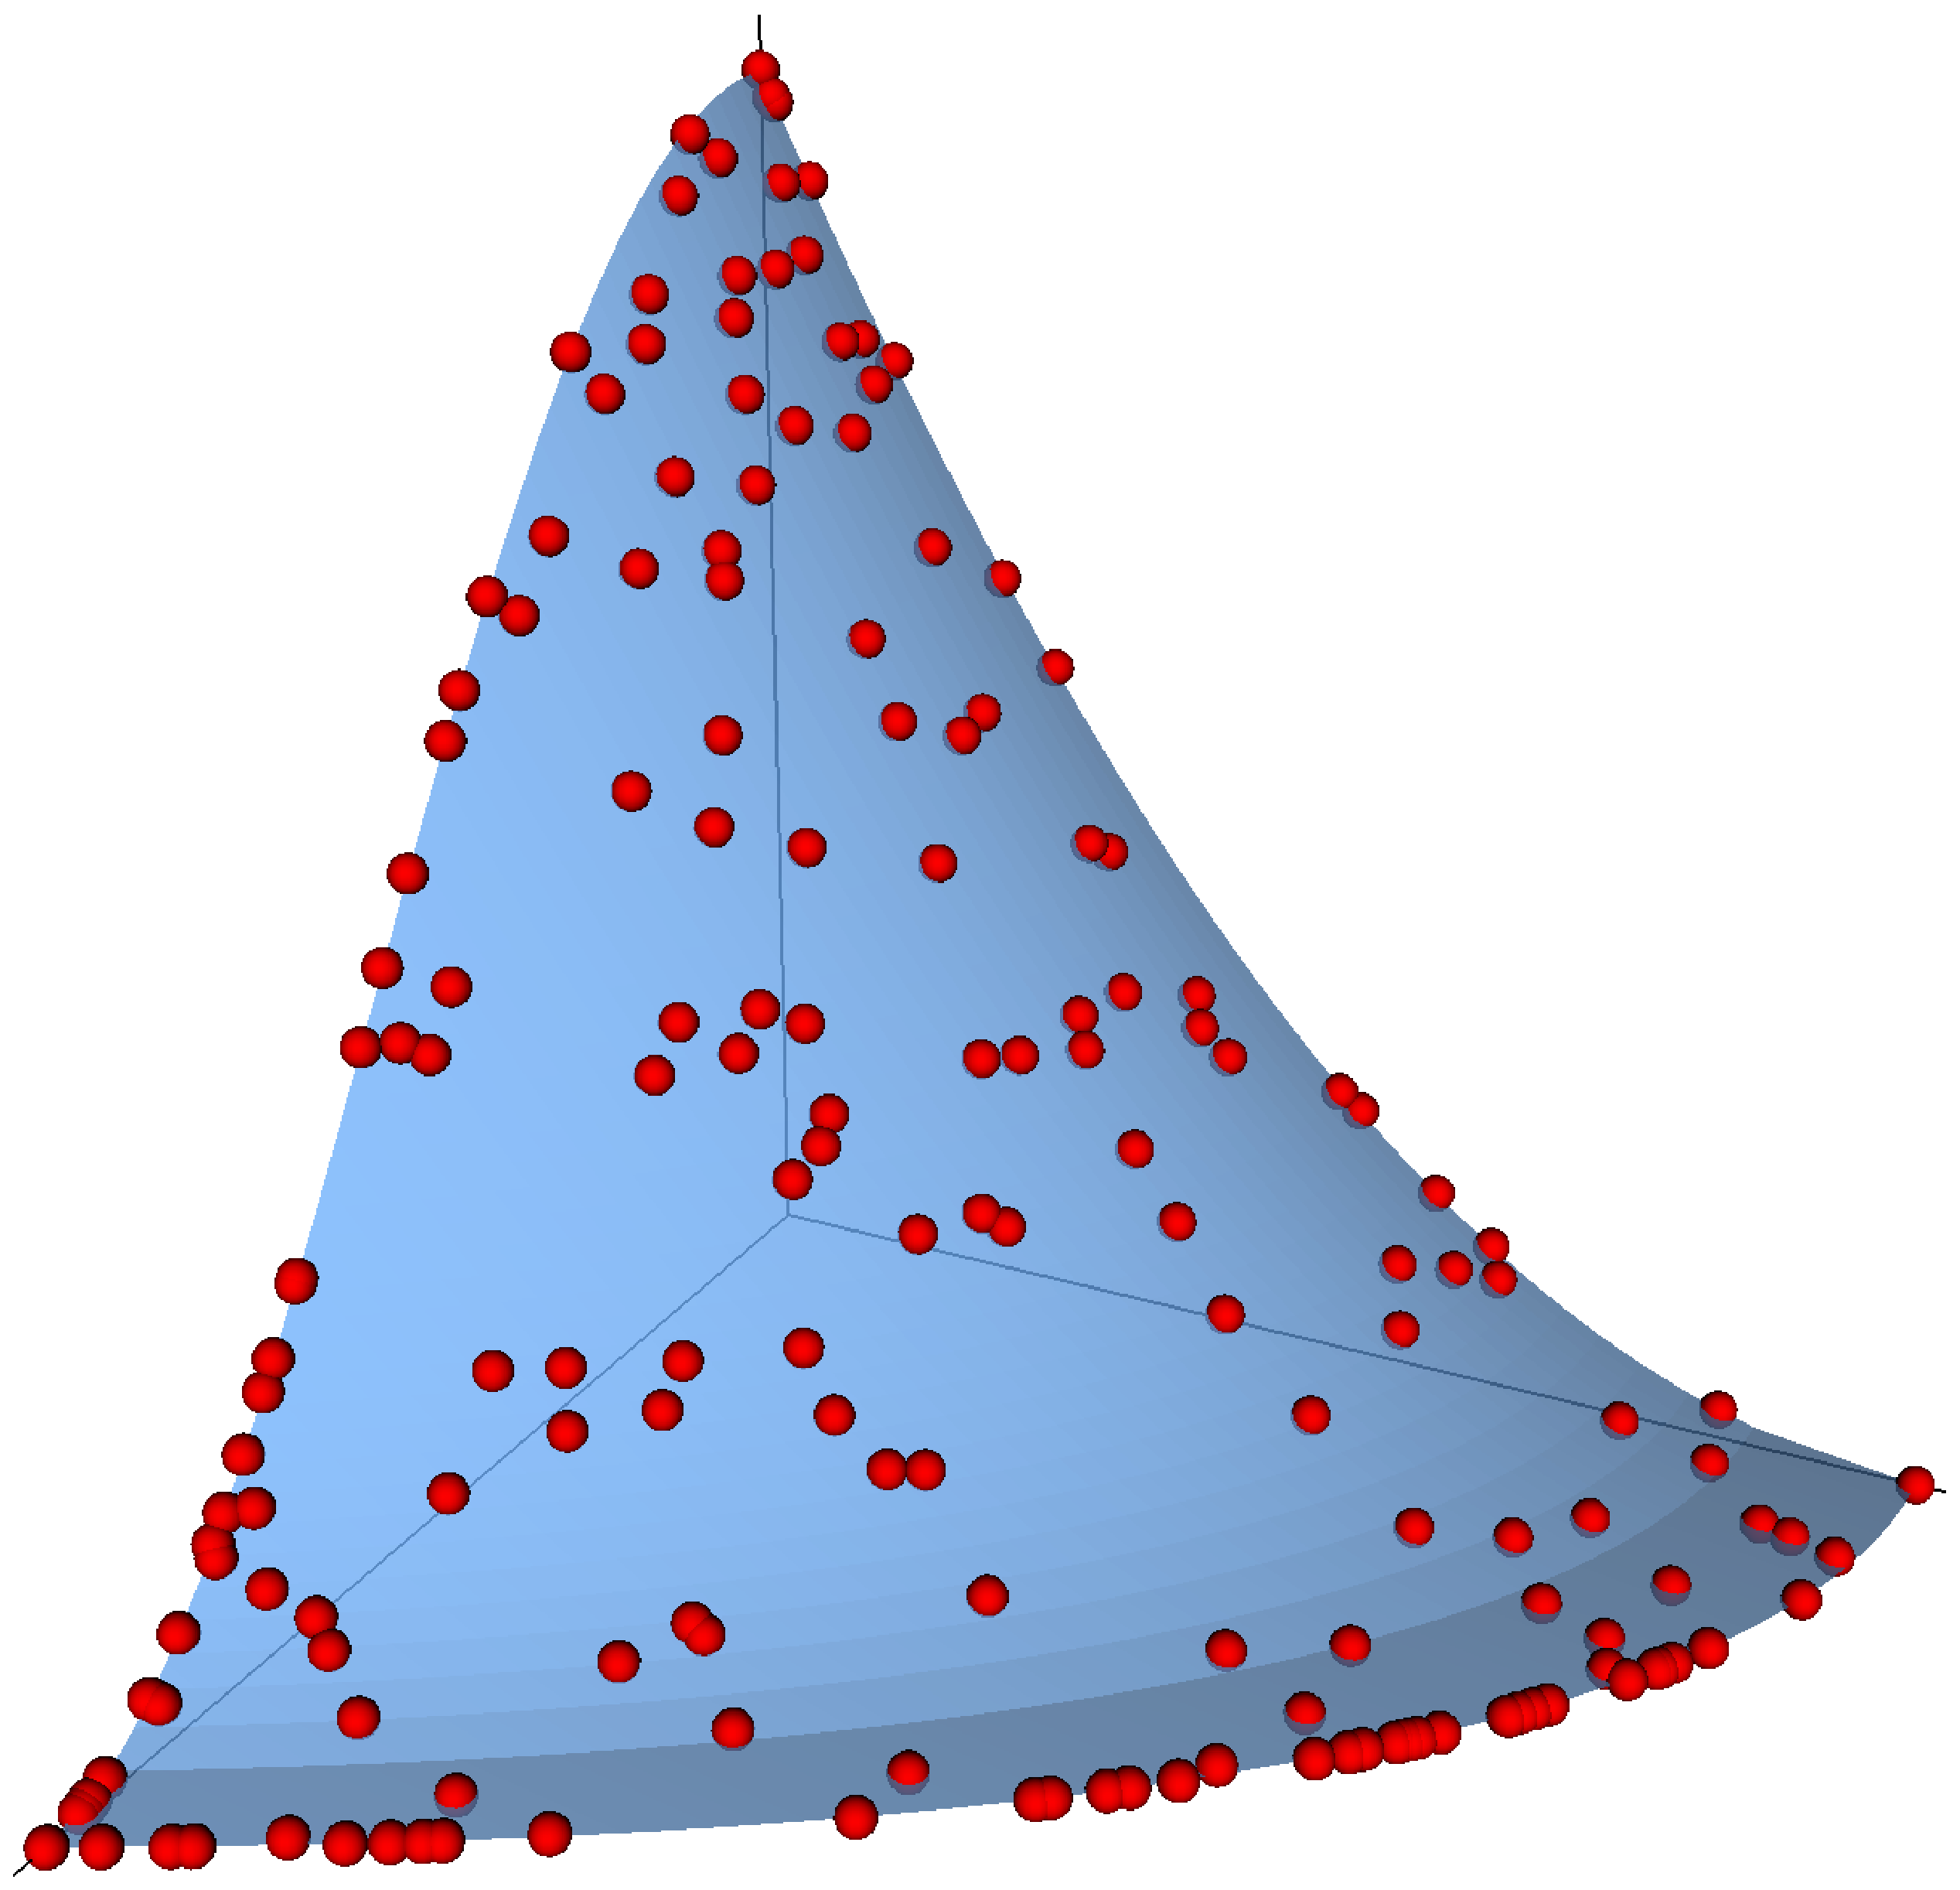
\includegraphics[width=0.36\linewidth]{./figs/res/vtk_SUQ2_A.eps}}
\subcaptionbox{SUQ2   (view 2)\label{fig:SUQ2_B}  }[0.49\linewidth]{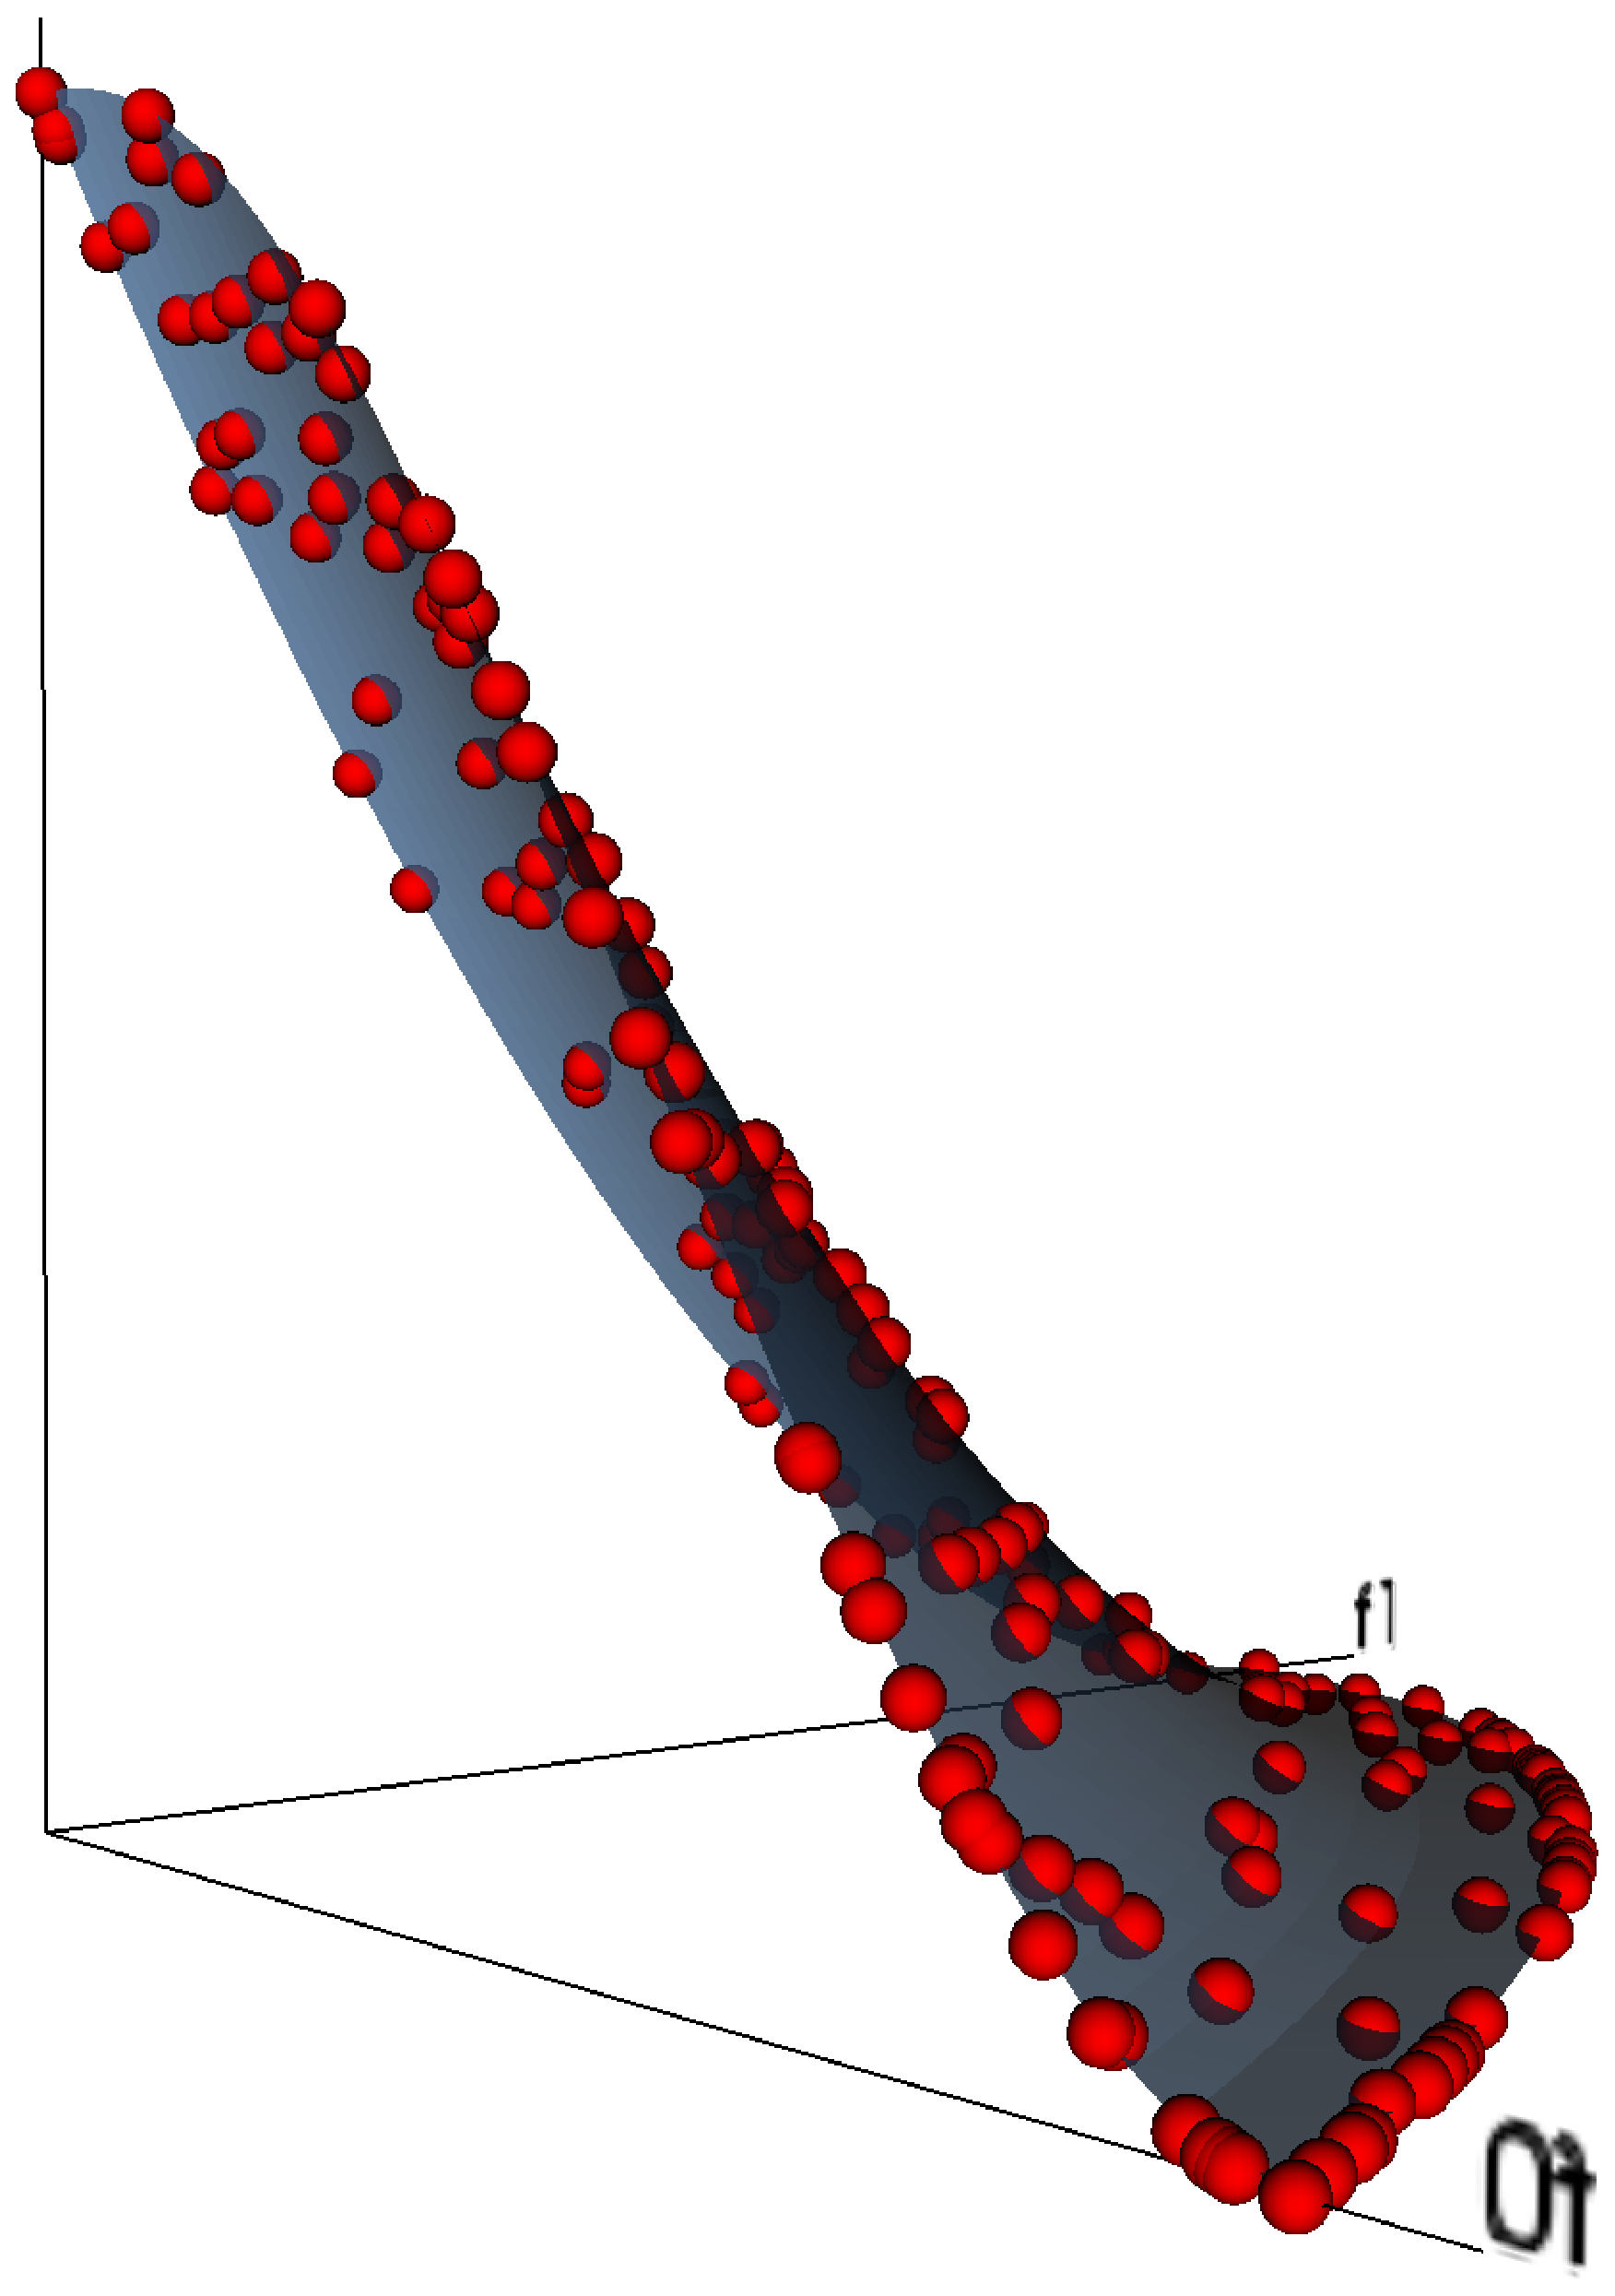
\includegraphics[width=0.26\linewidth]{./figs/res/vtk_SUQ2_B.eps}}
\caption{Three-objective problems (contd.).}% (a) DTLZ2c (view 1). (b) DTLZ2c (view 2). (c) SUQ1
%(view 1). (d) SUQ1 (view 2). (e) SUQ2 (view 1). (f) SUQ2 (view 2).}
\label{fig:three-objB}
\end{figure*}


A \emph{starplot} is employed to assist on verifying the ability of the code to cover all objective
functions. For each feasible trial solution with $\phi=0$ (best Pareto-optimal front), a line plot
is drawn by connecting the $f_i$ values. The axes for the $f_i$ values are drawn as in a star with
equal angles. The angle between axes is hence $\Delta\theta = 2\,\pi / N_f$. Because the $f_i$
points are connected, an area is created in the diagram. For reference, four circles are drawn; each
corresponding to a normalised objective value of $0.25$, $0.5$, $0.75$ and $1.0$. The normalisation
factor is equal to $1.0$ for all tests, except for DTLZ1 where it is equal to $0.5$. A good coverage
of objective functions is hence indicated by lines reaching the outer circles with high frequency.

The starplots for all DTLZi and SUQi tests are shown in \fignames~\ref{fig:three-objC} and \ref{fig:three-objD} where it
can be observed that the three objective values are well represented in all tests. Symmetry is
observed in DTLZ1-4, DTLZ2c and SUQ1. The superquadric SUQ2 does not have any symmetry in
particular. It is interesting to observe the difference between DTLZ2x (convex) and SUQ1
(superquadric) with respect to symmetry. In DTLZ2c, the region of values is restricted because of
the constraint. In this case, the combination of $f_i$ values must be over $0.3$ and smaller than a
value close to $0.75$.

\begin{figure*} \centering
\subcaptionbox{DTLZ1 \label{fig:DTLZ1} }[0.49\linewidth]{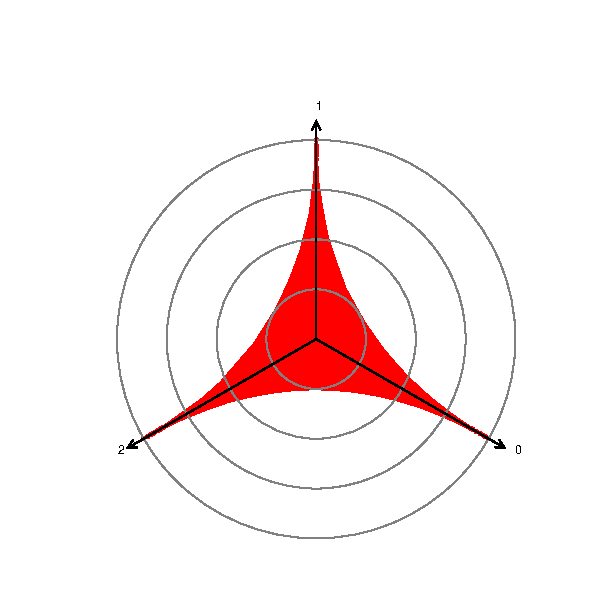
\includegraphics[width=0.34\linewidth,trim={45 17 25 25},clip]{./figs/res/starplot_DTLZ1.eps}}
\subcaptionbox{DTLZ2 \label{fig:DTLZ2} }[0.49\linewidth]{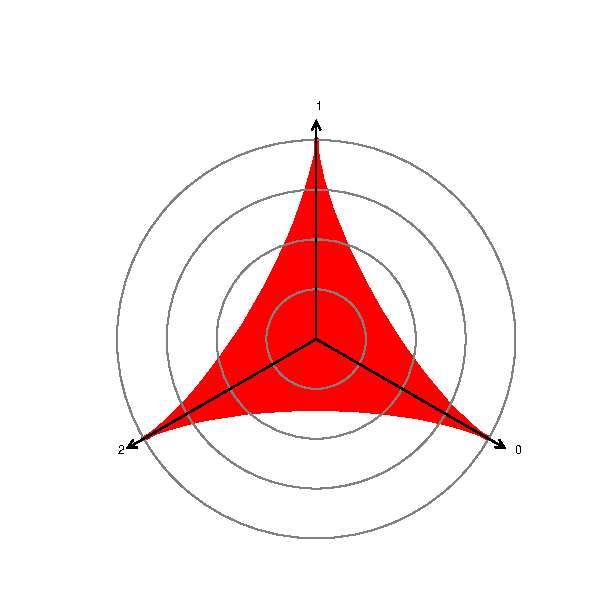
\includegraphics[width=0.34\linewidth,trim={45 17 25 25},clip]{./figs/res/starplot_DTLZ2.eps}}
\subcaptionbox{DTLZ3 \label{fig:DTLZ3} }[0.49\linewidth]{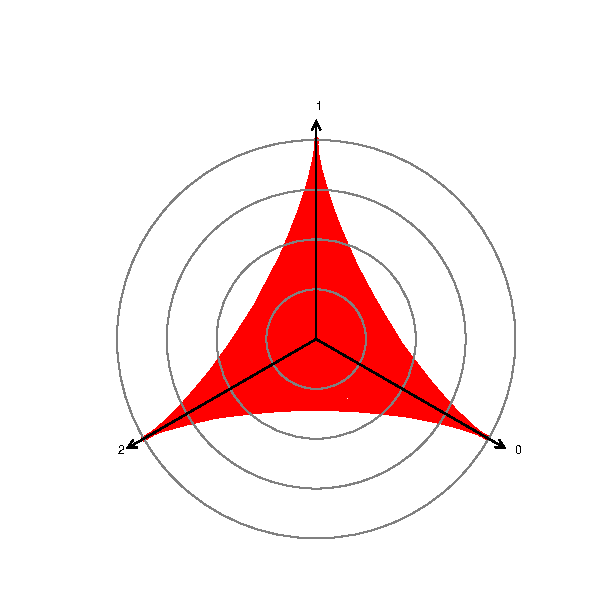
\includegraphics[width=0.34\linewidth,trim={45 17 25 25},clip]{./figs/res/starplot_DTLZ3.eps}}
\subcaptionbox{DTLZ4 \label{fig:DTLZ4} }[0.49\linewidth]{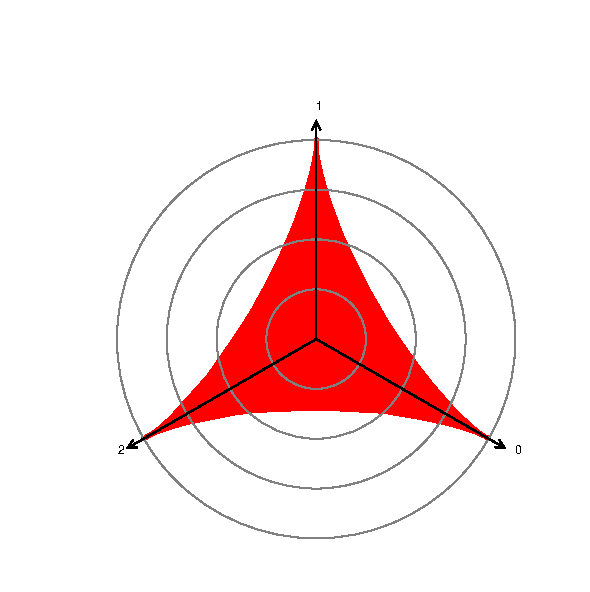
\includegraphics[width=0.34\linewidth,trim={45 17 25 25},clip]{./figs/res/starplot_DTLZ4.eps}}
\subcaptionbox{DTLZ2x\label{fig:DTLZ2x}}[0.49\linewidth]{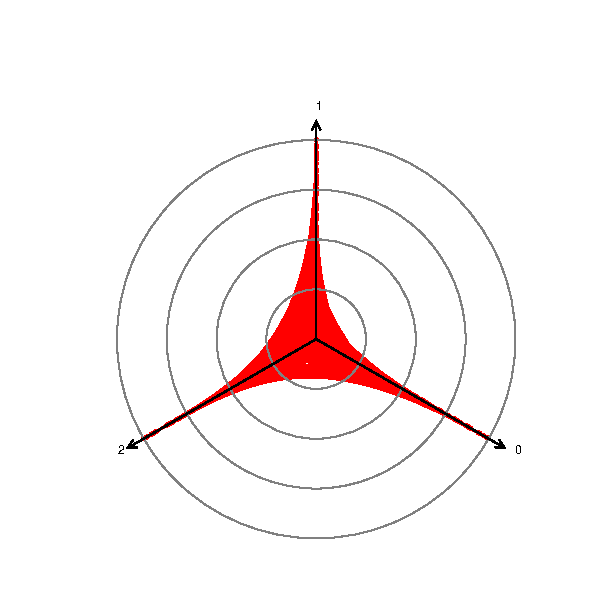
\includegraphics[width=0.34\linewidth,trim={45 17 25 25},clip]{./figs/res/starplot_DTLZ2x.eps}}
\subcaptionbox{DTLZ2c\label{fig:DTLZ2c}}[0.49\linewidth]{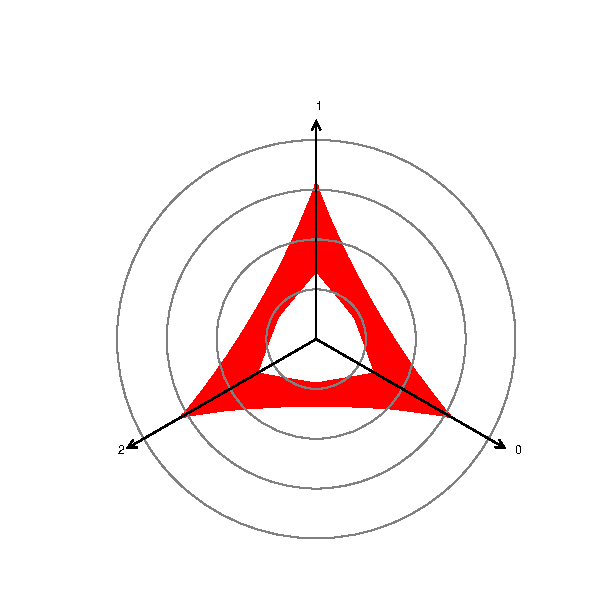
\includegraphics[width=0.34\linewidth,trim={45 17 25 25},clip]{./figs/res/starplot_DTLZ2c.eps}}
\caption{Three-objective problems. Starplots.}
\label{fig:three-objC}
\end{figure*}

\begin{figure*} \centering
\subcaptionbox{SUQ1  \label{fig:SUQ1}  }[0.49\linewidth]{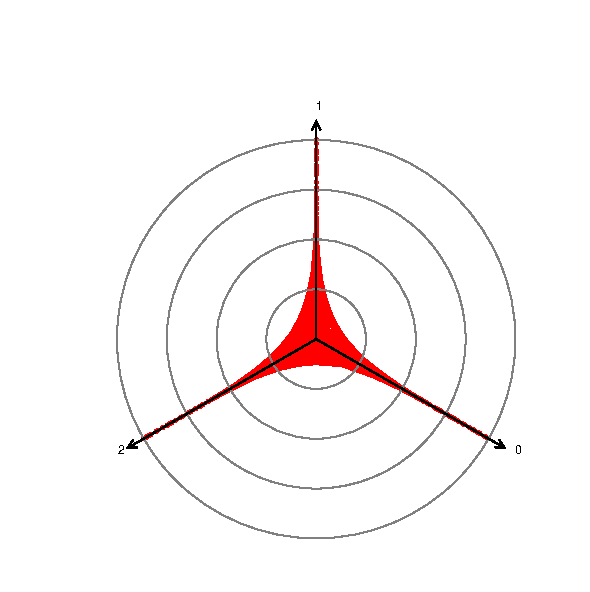
\includegraphics[width=0.34\linewidth,trim={45 17 25 25},clip]{./figs/res/starplot_SUQ1.eps}}
\subcaptionbox{SUQ2  \label{fig:SUQ2}  }[0.49\linewidth]{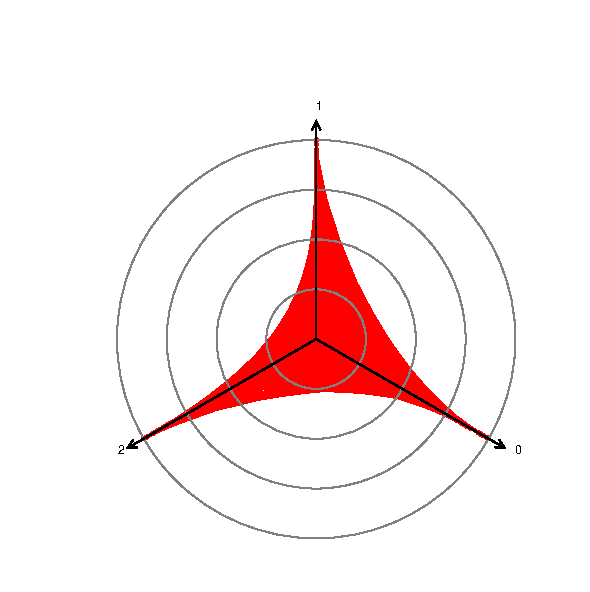
\includegraphics[width=0.34\linewidth,trim={45 17 25 25},clip]{./figs/res/starplot_SUQ2.eps}}
\caption{Three-objective problems. Starplots (contd.).}
\label{fig:three-objD}
\end{figure*}

To assess the accuracy and repeatability of results, 1000 samples are run for each problem and the
statistics with respect to the root mean square error are computed. The results are collected in
Table~\ref{tab:three-obj:A}. It can be observed that the errors and standard deviations reached
machine precision with the exception of DTLZ3 which is a little harder due to the local optima. With
more iterations, the error is reduced. The constraint in DTLZ2c does not cause problems to the
solver; remember that the algorithm prioritises satisfaction of constraints first hence trial
solutions are `pulled' into the conical space.

\import{./}{res-three-obj.tex}



\section{Test cases: many objective}
\label{sec:multiObj}

A final set of tests is carried out prior to the applications. Now, problem DTLZ2 is re-analysed
with more than 3 objectives. The following numbers of are selected: ${N_f \in \{5, 7, 10, 15,
20\}}$. The number of variables is also increased according to
\begin{equation}
    N_x = N_f + 10
\end{equation}
Thus, ${N_x \in \{15, 17, 20, 35\}}$. The number of trial solutions is $N_{sol}=300$ and 6 groups
are employed. It is clear that the problem with more objectives and variables are more difficult to
be solved. The problems are identified as \emph{DTLZ2mI} where $I$ means the number of objectives.

The starplots corresponding to the DTLZ2mI tests are illustrated in \figname~\ref{fig:many-obj}
where it can be observed that all objective values are found. As an exception, tests with 13 or more
objective values have less values reaching 1. Note that the number of trial solutions was kept
constant and equal to 300. With a few more iterations ($t_{max}$) and number of variables, the
response would be improved. This has not been done here for the sake of showing how the difficulty
increases with the number of objective functions.

\begin{figure*} \centering
\subcaptionbox{DTLZ2m5 \label{fig:DTLZ2m5} }[0.49\linewidth]{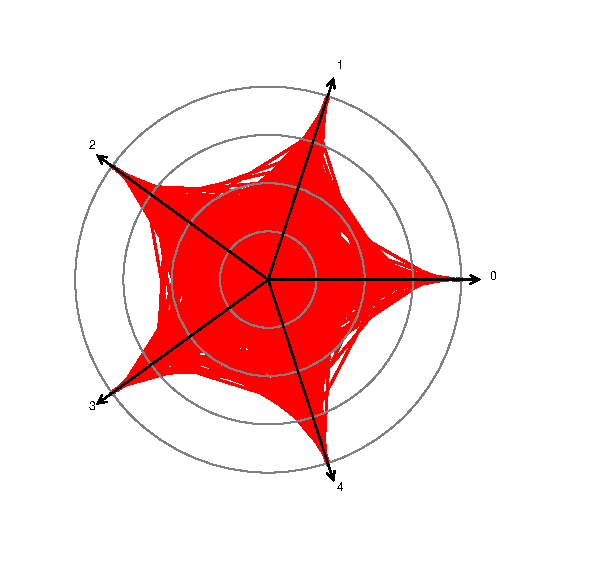
\includegraphics[width=0.34\linewidth,trim={25 35 25 20},clip]{./figs/res/starplot_DTLZ2m5.eps}}
\subcaptionbox{DTLZ2m7 \label{fig:DTLZ2m7} }[0.49\linewidth]{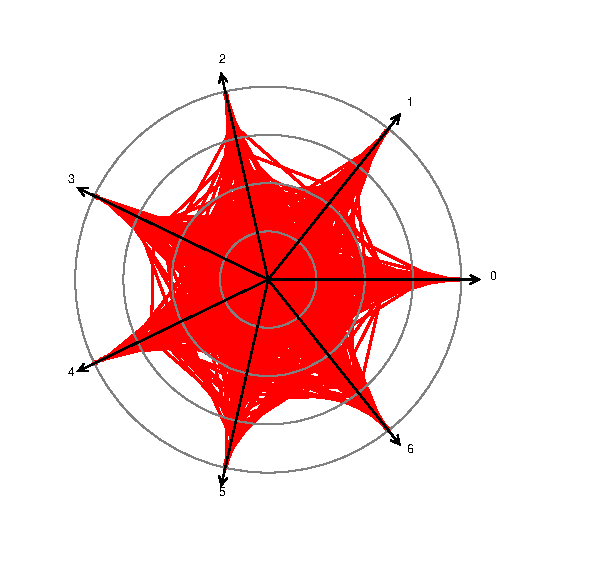
\includegraphics[width=0.34\linewidth,trim={25 33 25 18},clip]{./figs/res/starplot_DTLZ2m7.eps}}
\subcaptionbox{DTLZ2m10\label{fig:DTLZ2m10}}[0.49\linewidth]{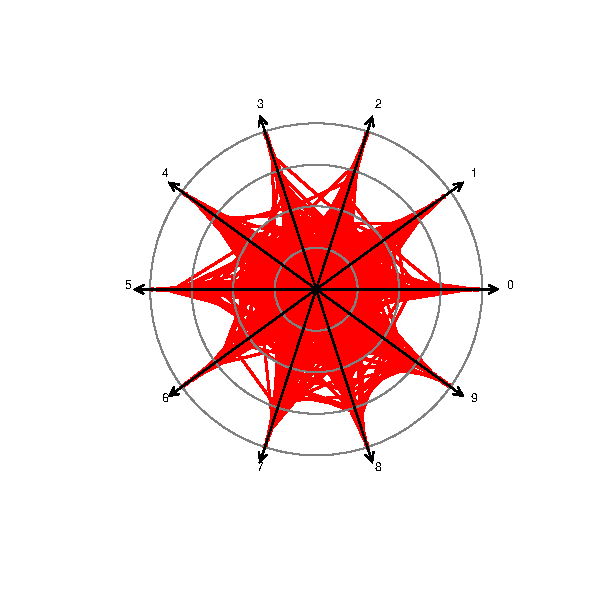
\includegraphics[width=0.34\linewidth,trim={50 50 25 30},clip]{./figs/res/starplot_DTLZ2m10.eps}}
\subcaptionbox{DTLZ2m13\label{fig:DTLZ2m13}}[0.49\linewidth]{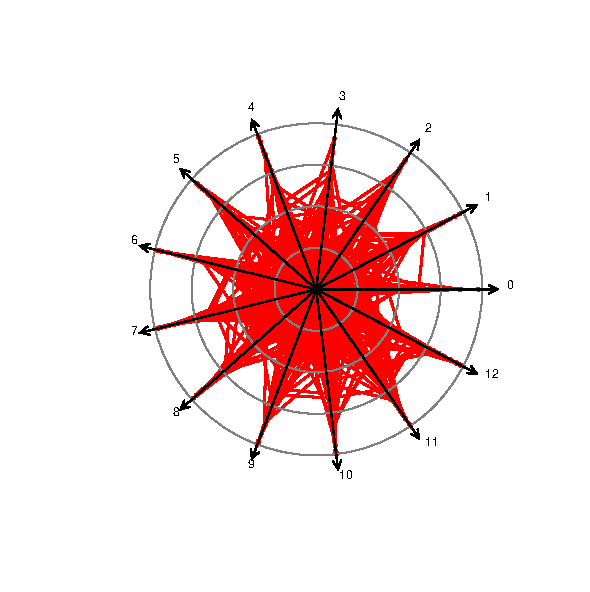
\includegraphics[width=0.34\linewidth,trim={50 45 25 30},clip]{./figs/res/starplot_DTLZ2m13.eps}}
\subcaptionbox{DTLZ2m15\label{fig:DTLZ2m15}}[0.49\linewidth]{\includegraphics[width=0.34\linewidth,trim={50 45 25 30},clip]{./figs/res/starplot_DTLZ2m15.eps}}
\subcaptionbox{DTLZ2m20\label{fig:DTLZ2m20}}[0.49\linewidth]{\includegraphics[width=0.34\linewidth,trim={50 45 25 30},clip]{./figs/res/starplot_DTLZ2m20.eps}}
\caption{Many-objective problems. Starplots.}
\label{fig:many-obj}
\end{figure*}

With regards to the statistics of errors, Table~\ref{tab:many-obj:A} presents the results for 1000
samples. As shown in this table, it is remarkable the ability of the proposed evolutionary algorithm
to obtain very small errors every time it is run. We observe in particular that the error increases
in a nonlinear trend with the number of objective functions; this is plotted in
\figname~\ref{fig:multierror}. It is actually interesting to see that the error rate decreases a
little considering that the number of trial solutions and iterations was kept constant. This means
that the performance of the code is reasonable for these tests.

\import{./}{res-many-obj.tex}

\begin{figure} \centering
\includegraphics[scale=1]{./figs/res/multierror.eps}
\caption{DTLZ2mI: Increase of error with number of objectives.}
\label{fig:multierror}
\end{figure}



\section{Application: truss shape and topology optimisation with two objectives}
\label{sec:topology}

The topology optimisation problem is an important one in structural engineering design. This problem
is even more difficult to be solved when the cross sectional areas of structural members (rods) have
to be found at the same time as the connections between rods. The problem is known as shape and
topology optimisation of trusses made up of slender rods (bars). A two objective version of this
problem is considered here. The two objectives are: (1) minimum deflection when the structure is
under loads; and (2) the overall minimum weight. Better satisfying one goal induces a failure in
satisfying the other one. Hence a Pareto optimal front is to be determined. The structure has to be
stable as well; therefore limits on maximum stresses must be followed hence defining constraints.

To solve this problem, a combination of real numbers and integers is implemented. The equilibrium of
the structure is solved by the finite element method (FEM) and a method to handle failures of the
FEM calculations is developed. The speedup that can be achieved with the resulting parallel code is
also demonstrated in this section.

The example studied in \citep{ruy:01, deb:01a, wu:10, noi:13, cazacu:14} and illustrated in
\figname~\ref{fig:truss} is considered. The Young's modulus of all bars is $E=10^4$ [units of
pressure] and the density is $\rho=0.1$ [units of density]. In this figure, the structure is known
as \emph{ground} structure because it serves as a basis for the generation of other combinations. It
is important to note that a minimum number of joints (nodes) and bars (elements) must be present at
all times in order to allow the structure to carry the prescribed load. In this particular problem,
the indicated fixed nodes and the nodes where loads are applied must be always present. Therefore,
before solving the mechanical problem, the connectivity has to be checked.

\begin{figure} \centering
\includegraphics[scale=1]{./figs/mesh-ground10.eps}
\caption{``Ground'' mesh with all 10 rods active.}
\label{fig:truss}
\end{figure}

Even if all required nodes are present, the structure may become a mechanism (or mobile). In this
situation, the FEM solver will fail due to a singular global stiffness matrix. To minimise the
number of unsuccessful calls to the FEM solver, a \emph{mobility} number $M$ can be estimated. In
this work, the Chebychev-Gr\"{u}bler-Kutzbach criterion is employed to this task \citep{gogu:05,
li:15}. For the truss system, $M$ is defined as
\begin{equation}
    M = 2\,n - m - \chi
\label{eqn:mobility}
\end{equation}
where $n$ is the number of nodes, $m$ is the number of bars and $\chi$ is the number of fixed
degrees of freedom. For instance, in the structure of \figname~\ref{fig:truss}, $n=6$, $m=10$ and
$\chi=4$ because $\{u_x,u_y\}$ at $(0.0,0.0)$ and $(0.0,360.0)$ are fixed. If $M$ is positive, the
above expression indicates that the structure is a mechanism/mobile. Nonetheless, the expression may
fail at times for instance when there are redundant bars at some locations and some local mechanisms
arise at other locations. Therefore, the above condition is not sufficient and yet a singular global
stiffness matrix (or the failure of the FEM) must be properly handled.

The problem representation is as follows. Integers are used for the topology description (connection
of bars) and real numbers for the cross sectional areas. In this case, integers simply serve as
Boolean variables where 1 means a connection is active and 0 otherwise. There are 10 bars (10
areas); thus the number of real numbers $\vx$ is $N_x=10$ and the number of integers $\vksi$ is
$N_\xi=10$. The limits are
\begin{equation}
    0.09 \leq x_i \leq 35 \quad i \in [0,9]
\end{equation}
indicating that the minimum and maximum areas are 0.09 and 35 [units of area], respectively.

The objective values ($f_0$: total weight; $f_1$: deflection) are computed after running a finite
element (FEM) simulation to calculate the maximum deflection ${\delta=|u_y^{max}|}$ at ${x=720}$ and
${y=0}$. This value is also limited by a maximum allowance of ${\delta_{awd}=5.6}$ [units of
displacement]. The maximum allowed tensile or compressive axial stress $\sigma_{max}$ (from FEM) at
any bar is ${\sigma_{awd}=35}$ [units of pressure]. The bar lengths are $L_i$.

Considering the general optimisation problem \eqname~(\ref{eqn:optGeneral}), the required
expressions are (with ${f_i=f_i(\vx,\vksi)}$ and ${u_i=u_i(\vx,\vksi)}$)
\begin{align}
    f_0 &= \sum_{i=0}^{N_{active}} \rho \, x_i \, L_i \ACR
    f_1 &= \delta                                     \ACR
    u_0 &= \ramp{M}                                   \ACR
    u_1 &= \text{1 if FEM failed; 0 otherwise}        \ACR
    u_2 &= \ramp{\delta - \delta_{awd}}               \ACR
    u_3 &= \ramp{|\sigma_{max}| - \sigma_{awd}}
\end{align}
There are four constraints (out-of-range/OOR) functions $u_i$. In the above equation, $\ramp{x}$ is
the ramp function defined by
\begin{equation}
    \ramp{x} = \left\{\begin{matrix}
        0 & \text{if $x<0$} \\
        x & \text{otherwise}
    \end{matrix}\right.
\end{equation}

The use of the OOR functions is quite convenient because, since the comparison between trial
solutions first considers the number of constraint violations $N_{viol}$, the OOR functions can be
set in a way such that the worst case gets the highest $N_{viol}$ value by assigning a greater than
zero $u_i$ values (e.g. $1.0$). Note also that the OORs are compared using the
\FnParetoComparison~which effectively ranks trial solutions even if the FEM solver is not called at
all. The proposed strategy is implemented as detailed in Algorithm~\ref{alg:femsim}.

In Algorithm~\ref{alg:femsim}, if not all vertices are present because connections cannot be made,
the OOR $u_0$ gets $1+2\,n$ which is a number greater than the maximum mobility $M$ (when there are
no bars and no fixities). In this situation, the other OORs all get $1.0$. Therefore, the first exit
condition in the algorithm will define a candidate that is worse than another one which could be at
least used to compute its mobility number. Note that the third exit condition is closer to a
situation needed to calculate the displacements and stresses; but still the FEM fails.


\import{./}{algo-09-femsim.tex}


The solution is obtained with \goga~where its good repeatability characteristics is verified again.
The other configuration parameters are as follow. Simple crossover and mutation rules for integers
are employed \citep{gold:89} with probability ${P_c=0.5}$ and ${P_m=0.01}$, respectively. The number
of cuts during crossover is 1 and the number of bit changes during mutation is 1. ${N_{sol}=200}$,
${t_{max}=500}$ and ${\Delta t_{exc}=50}$ are selected. The differential evolution coefficient value
$C_{DE}=0.8$ is selected. The number of groups $N_{cpu}$ is varied from 1 to 16 in order to study
the speedup characteristic.

A typical Pareto-optimal front obtained with \goga~is shown in \figname~\ref{fig:topoFront} where a
reference line from \citep{deb:01a} is also drawn (shown in blue). Five combinations of
weight-deflection values are indicated in the figure using labels `A' to `E' ranging from the
lightest structure to the heaviest one. The resulting structure corresponding to each label is drawn
in the same figure near the weight-deflection point (marked with a green star). Some examples of
trusses are drawn near the weight-deflection point (marked with a green star). In each drawing, the
thickness of the line is proportional to the optimal cross sectional area. We observe that the
results match the reference ones reasonably well. The computed areas corresponding to each selected
point are collected in \tabname~\ref{tab:topoFront}.

\begin{figure*} \centering
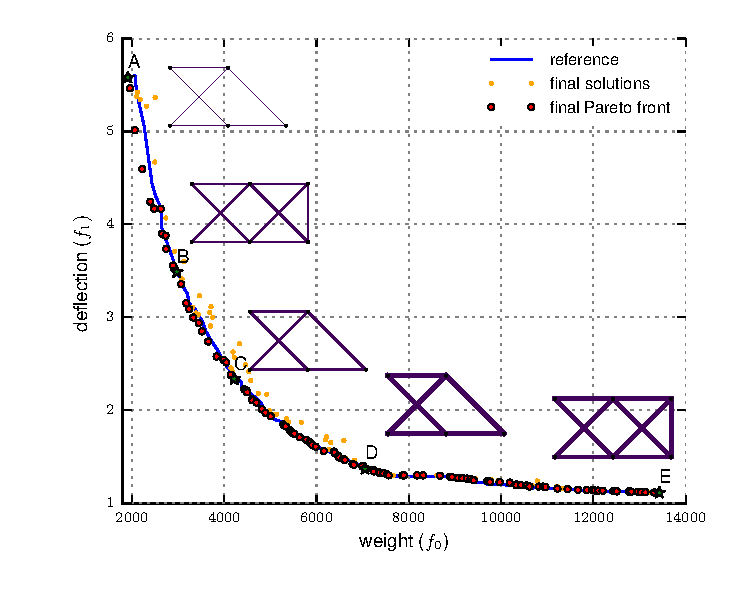
\includegraphics[scale=1]{./figs/res/ground10.eps}
\caption{Shape and topology optimisation. Results.}
\label{fig:topoFront}
\end{figure*}

\import{./}{res-ground10.tex}


The efficiency of the parallel strategy is now assessed by running the topology optimisation problem
sixteen times with different number of groups (CPUs). Simulations are carried out in a 16-core
Intel(R) Xeon(R) CPU E5-2687W @ 3.10GHz (Debian-Sid/GNU/Linux). The speedup is then computed by means
of
\begin{equation}
    S_{up}(N_{cpu}) = \frac{T_{sys}^1}{T_{sys}^{N_{cpu}}}
\end{equation}
where $T_{sys}^1$ is the computer time using one group (CPU) and $T_{sys}^{N_{cpu}}$ is the computer
time using $N_{cpu}$ groups. The results are plotted \figname~\ref{fig:topoSpeedup} where we can
observe a better than ideal speedup up to 14 CPUs. In the figure, the real computer time is also
shown in using a gray line with values given at the right-hand-side scale; the maximum time is
around 40 seconds, for instance.

The reason for the excellent speedup behaviour is in part due to a faster execution of the
non-optimised implementation of the \FnMetrics~routine. This routine needs to perform several
comparisons between trial solutions in order to find the closest neighbours in addition to determine
the Pareto front indices. For example, by disabling the FEM computations, a slightly similar
behaviour is observed where a very high speedup happens as well.

\begin{figure} \centering
\includegraphics[scale=1]{./figs/res/topology-speedup.eps}
\caption{Shape and topology optimisation. Speedup.}
\label{fig:topoSpeedup}
\end{figure}



\section{Application: economic emission load dispatch}
\label{sec:economic}

Economic emission load dispatch (or environmental/economic dispatch EED) is an interesting multi
objective optimisation problem of great importance in power generation. The problem involves the
design of optimal power flow observing the cost of operation and the emission of pollutants. These
two objectives are contradictory and a number of constraints such as the maximum capacity of
generators and the total power balance must be satisfied. The problem has been studied over several
years; for example, some papers from 1987 to 2015 are: \citep{yokoyama:87, farag:95, abido:03,
abido:06, alra:06, kumar:09, dhana:11, bayon:12, rahmat:13, li:13, jubril:13, bilil:14, jeddi:14,
jubril:14, sayah:14, bhatta:15, zhang:15}.

In the EED problem, the fuel cost $f_0$ of a thermal unit is approximated by the following quadratic
function
\begin{equation}
    f_0 = \sum_{i=0}^{N-1} \left( a_i + b_i\,P_i + c_i\,P_i^2 \right)
\end{equation}
where $N$ is the number of generators and ${x_i:=P_i}$ is the (unknown) active output power of
generator $i$. Therein, $a_i$, $b_i$ and $c_i$ are fitting parameters. The corresponding emission
$f_1$ is also modelled as a function of the power output by means of
\begin{equation}
    f_1 = \sum_{i=0}^{N-1} \left[
		 \alpha_i+\beta_i\,P_i+\gamma_i\,P_i^2 + \zeta_i\,\exp{(\lambda_i\,P_i)}
    \right]
\label{eqn:emission}
\end{equation}
where $\alpha_i$, $\beta_i$, $\gamma_i$, $\zeta_i$ and $\lambda_i$ are fitting parameters.

The power output $P_i$ is limited by the generation capacity. Moreover, an equality constraint $h_0$
must be taken into account in order to satisfy the power balance involving the total power
generation $\sum P_i$ of the system, the total load demand $P_{demand}$ and the total transmission
loss $P_{loss}$. The balance constraint is thus expressed by
\begin{equation}
    h_0 = \left(\sum_{i=0}^{N-1} P_i \right) - P_{demand} - P_{loss} \equiv 0
\end{equation}
The transmission loss $P_{loss}$ is a nonlinear function of the power outputs $P_i$ and requires
the solution of the power flow equations. It depends on other variables such as the bus voltage
magnitudes and angles. Nonetheless, a simple expression is available to approximate $P_{loss}$ as
follows
\begin{equation}
    P_{loss} = B_{00} + \sum_{i=0}^{N-1} B_{0i}\,P_i + \sum_{i=0}^{N-1} \sum_{j=0}^{N-1} P_i \, B_{ij} \, P_j
\end{equation}
where the $B_{ij}$ coefficients are derived for each particular bus case.

The specific economic-emission dispatch of the \emph{IEEE 30 Bus Test Case} is studied here. Its
sketch is presented in \figname~\ref{fig:IEEE30bus} and is based on \citep{yokoyama:87}. The
required fitting parameters are listed in Table~\ref{tab:IEEE30busPrms} including the capacity
limits. These values are based on data from \citep{yokoyama:87} and \citep{abido:03} (note that
there is a typo error in \citep{abido:03} with regards to the $\alpha$ coefficient for $G_4$ in
Table~1 of that paper).

The demand load considered in the EED problem is $P_{demand}=2.834$ and the $B$ coefficients for the
IEEE 30 Bus Test case are collected in Table~\ref{tab:IEEE30busBcoefs} \citep{wang:08, ozyon:12,
pal:12}.

\begin{figure} \centering
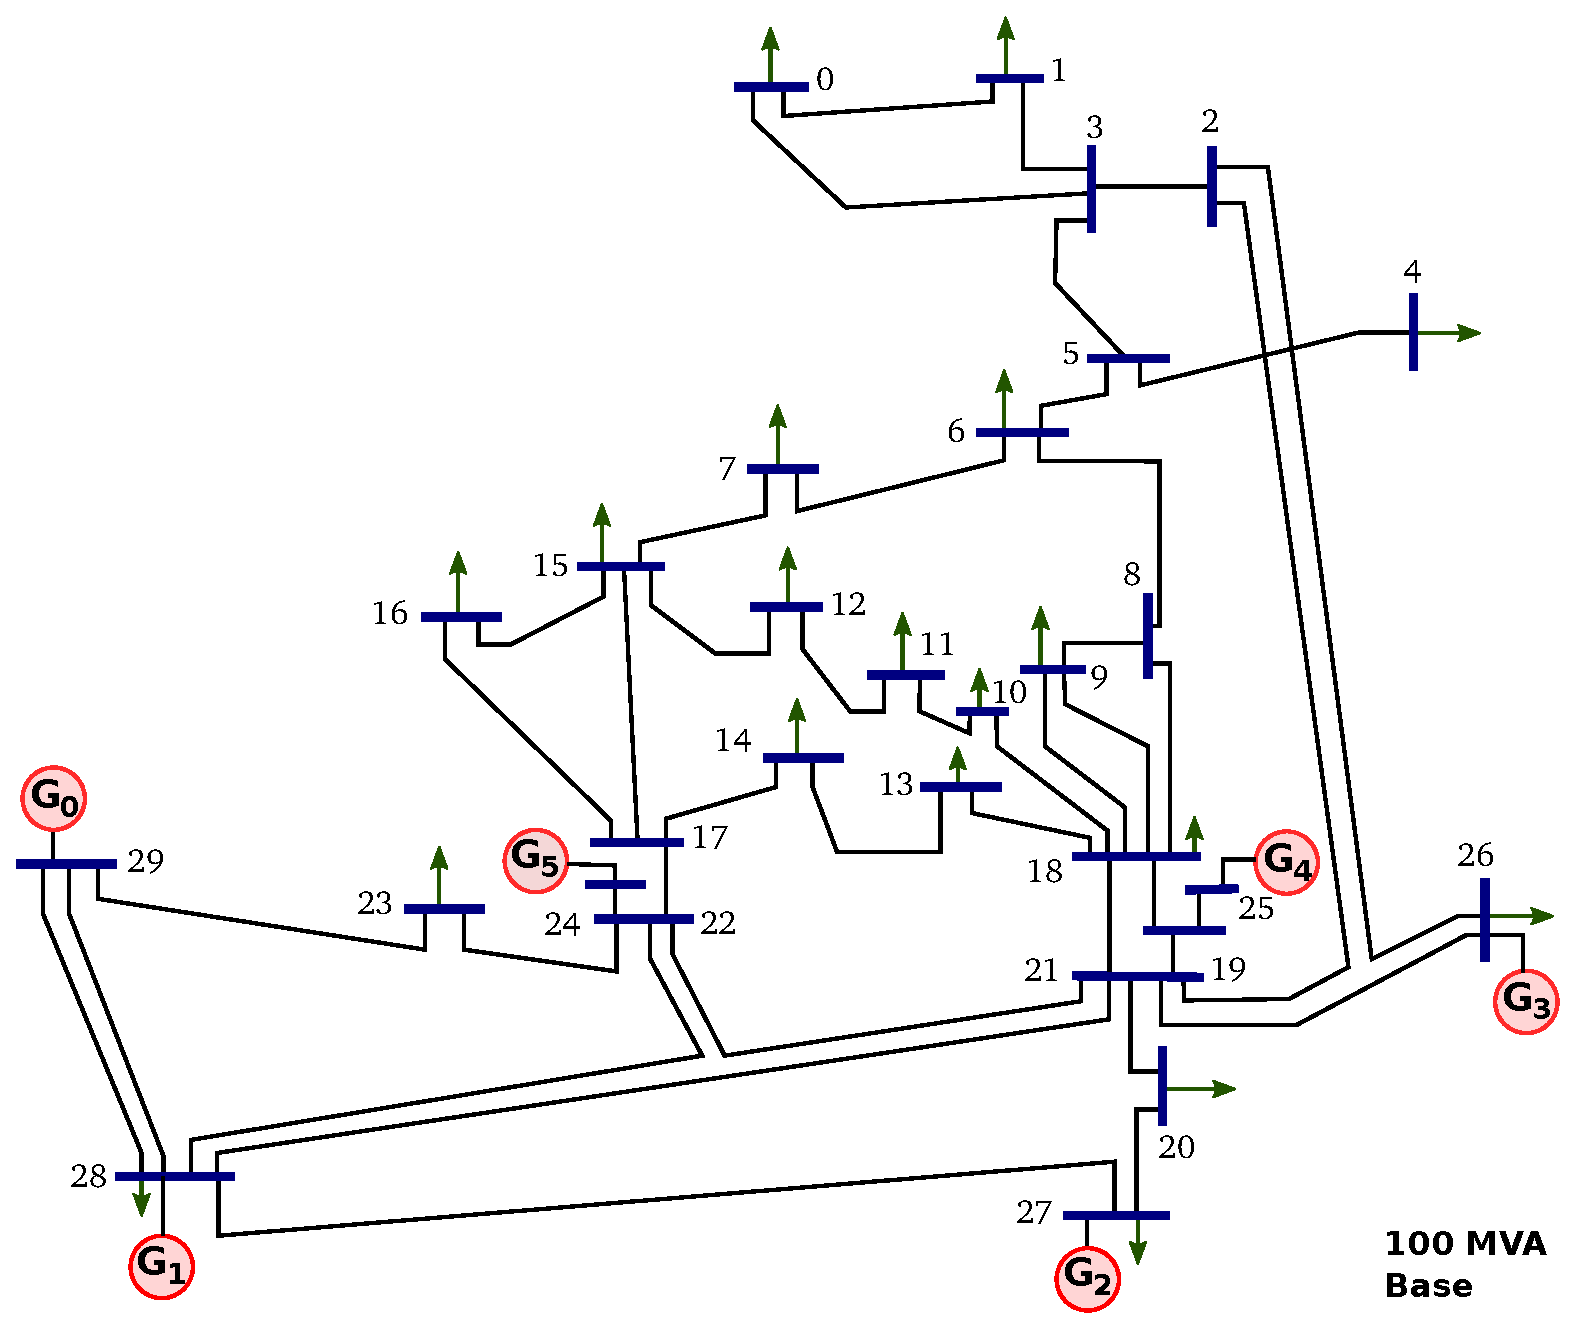
\includegraphics[width=\linewidth]{./figs/IEEE30bus.eps}
\caption{IEEE 30 bus test system.}
\label{fig:IEEE30bus}
\end{figure}

\IEEEthirtyBusPrms

\IEEEthirtyBusBcoefs

Two cases are considered: a lossless and a lossy situation. In the first one, $P_{loss}$ is set to
zero making the problem a little easier. The solution is obtained with ${N_{sol}=200}$,
${t_{max}=500}$, ${N_{cpu}=4}$ and ${\Delta t_{exc}=50}$. In addition, the control for the equality
constraint $h_0$ is ${\epsilon_h=10^{-3}}$ and the differential evolution coefficient is
$C_{DE}=0.8$.

The Pareto-optimal front for the first case (lossless) is illustrated in
\figname~\ref{fig:eedLossless} where it can be observed that the results match well the reference
solution from \citep{abido:06}. The optimal front for the second case (lossy) is illustrated in
\figname~\ref{fig:eedLossy} where the reference solution from \citep{abido:06} is slightly less
optimal than the one computed here.

In both figures, some points corresponding to the minimum cost, a compromise between cost and
emission, and the minimum emission are indicated using labels `A', `B' and `C', respectively. The
generators power corresponding to these selected points are listed in Table~\ref{tab:eedLossless}
for the lossless case and in Table~\ref{tab:eedLossy} for the lossy case. The balance errors are
also listed in these tables under the $h_0$ column. We observer that the errors fall within the
range specified by $\epsilon_h$ as required. It is also interesting to observe that the cost is
higher for the lossy case than for the lossless case; a reasonable fact.

\begin{figure} \centering
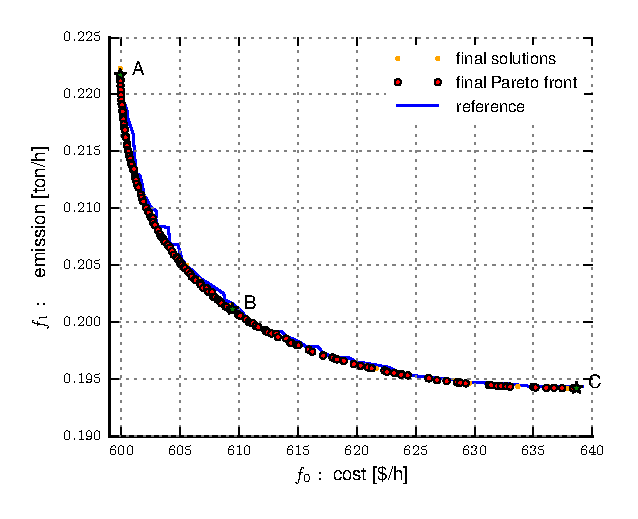
\includegraphics[width=\linewidth]{./figs/res/ecoemission_prob3.eps}
\caption{Economic emission load dispatch. Lossless.}
\label{fig:eedLossless}
\end{figure}

\begin{figure} \centering
\includegraphics[width=\linewidth]{./figs/res/ecoemission_prob4.eps}
\caption{Economic emission load dispatch. Lossy case.} 
\label{fig:eedLossy} 
\end{figure}

\import{./}{res-eed-prob3.tex}

\import{./}{res-eed-prob4.tex}



\section{Conclusions}

This paper presented an evolutionary algorithm using differential evolution capable of solving a
range of optimisation problems, including some with many constraints and more than one objective.
Several tests are studied including optimisation problems with up to 20 objective functions. The
Pareto optimality is employed for these functions. The repeatability of the code is demonstrated by
observing a small standard deviation from several runs with the same problem but different initial
trial solutions. This characteristic is essential to obtain a level of reliability of the code.

Two applications are studied: topology optimisation of trusses and the economic emission dispatch.
For the first one, it is shown that the use of the out-of-range functions helps with the handling of
constraints and failures due to calls to the finite element solver that are required to compute the
objective values. The second application involves an equality constraint (the power balance) that
makes the problem a little more challenging. Nonetheless, it is demonstrated that the proposed code
works well with both applications.

The algorithm is designed to be used in multiple-core machines and be run in parallel. This is
accomplished by splitting the space of trial solutions into smaller groups, each one running in
parallel until a time for exchange of solutions is reached. Two strategies for exchanging solutions
are combined: by tournament and randomly. These two strategies help with widening the search space
in addition to making computations faster. Evidence of the good characteristics of the proposed code
including the ideal speedup properties are also shown.


\section*{Acknowledgment}

The support from the Australian Research Council under grant DE120100163 is gratefully acknowledged.


%% The Appendices part is started with the command \appendix;
%% appendix sections are then done as normal sections
%% \appendix

%% \section{}
%% \label{}

%% References
%%
%% Following citation commands can be used in the body text:
%% Usage of \cite is as follows:
%%   \cite{key}          ==>>  [#]
%%   \cite[chap. 2]{key} ==>>  [#, chap. 2]
%%   \citet{key}         ==>>  Author [#]

%% References with bibTeX database:

\bibliographystyle{model3-num-names}
\bibliography{mydatabase}

%% Authors are advised to submit their bibtex database files. They are
%% requested to list a bibtex style file in the manuscript if they do
%% not want to use model3-num-names.bst.

%% References without bibTeX database:

% \begin{thebibliography}{00}

%% \bibitem must have the following form:
%%   \bibitem{key}...
%%

% \bibitem{}

% \end{thebibliography}


\end{document}

%%
%% End of file `elsarticle-template-3-num.tex'.
